% Customizable fields and text areas start with % >> below.
% Lines starting with the comment character (%) are normally removed before release outside the collaboration, but not those comments ending lines

% svn info. These are modified by svn at checkout time.
% The last version of these macros found before the maketitle will be the one on the front page,
% so only the main file is tracked.
% Do not edit by hand!
\RCS$Revision: 303178 $
\RCS$HeadURL: svn+ssh://svn.cern.ch/reps/tdr2/notes/AN-15-114/trunk/AN-15-114.tex $
\RCS$Id: AN-15-114.tex 303178 2015-09-09 07:46:54Z chwalek $
%%%%%%%%%%%%% local definitions %%%%%%%%%%%%%%%%%%%%%
% This allows for switching between one column and two column (cms@external) layouts
% The widths should  be modified for your particular figures. You'll need additional copies if you have more than one standard figure size.
% superseded by ptdr-definitions.sty



  \newcommand{\costhetalj}{\cosThetaPol}
  %\renewcommand{\mu}{\ensuremath{\mu}\xspace}
  \newcommand{\e}{\ensuremath{\mathrm{e}}\xspace}
  \newcommand{\topMass}{\mt}
%  \newcommand{\mtw}{\ensuremath{m_{Tw}}\xspace}
  \newcommand{\invpb}{\ensuremath{pb^{-1}}\xspace}


    \newcommand{\sigmatch}{\ensuremath{\sigma_{t-\mathrm{ch.}}}\xspace}
  \newcommand{\mt}{\ensuremath{m_{\ell\nu \mathrm{b}}}\xspace}
  \newcommand{\mlbnu}{\mt}
  \newcommand{\cosThetaPol}{\ensuremath{\cos{\theta^*}}\xspace}
  \newcommand{\etalj}{\ensuremath{|\eta_{j^\prime}|}\xspace}
  \newcommand{\vtb}{\ensuremath{V_{\mathrm{tb}}}\xspace}
  \newcommand{\vtbAbs}{\ensuremath{|V_{\mathrm{tb}}|}}
  \newcommand{\met}{\ensuremath{{E\!\!\!/}_{\mathrm{T}}}\xspace}
  \renewcommand{\MET}{\met}
  \newcommand{\PFrelIso}{\ensuremath{I_{\mathrm{rel}}}\xspace}
  \newcommand{\PFrelIsoRho}{\ensuremath{I_{\mathrm{rel}^{\rho corr.}}}\xspace}
  \newcommand{\pfPhotonIso}{\ensuremath{I^{\gamma}}\xspace}
  \newcommand{\pfChargedHadronIso}{\ensuremath{I^{\mathrm{ch.\,h}}}\xspace}
  \newcommand{\pfNeutralHadronIso}{\ensuremath{I^{\mathrm{n.\,h}}}\xspace}
  \newcommand{\pfPU}{\ensuremath{I^{\mathrm{PU}}\xspace}}
  \newcommand{\sumPUPT}{\ensuremath{\sum p_T^{PU}}\xspace}
  \newcommand{\sumPUPt}{\sumPUPT}
  \newcommand{\rhoEnergy}{\ensuremath{\rho \times A}}
  \newcommand{\mTW}{\ensuremath{m_{\mathrm{\rm T}}^{\rm W}}\xspace}
  \newcommand{\mtw}{\ensuremath{m_{\mathrm{\rm T}}}\xspace}
  \newcommand{\mW}{\ensuremath{m_{\mathrm{\rm W}}}\xspace}
  \newcommand{\mT}{\ensuremath{m_{\mathrm{\rm T}}}\xspace}
  \newcommand{\qcd}{\ensuremath{\rm QCD}\xspace}
  \newcommand{\QCD}{\qcd}
  \newcommand{\wjets}{\ensuremath{\textrm{W+jets}}\xspace}
  \newcommand{\WJets}{\wjets}
  \newcommand{\zjets}{\ensuremath{\textrm{Z+jets}}\xspace}
  \newcommand{\ZJets}{\zjets}
  \newcommand{\vjets}{\ensuremath{\textrm{V+jets}}\xspace}
  \newcommand{\VJets}{\vjets}
  \newcommand{\wzjets}{\ensuremath{\textrm{W/Z+jets}}\xspace}
  \newcommand{\WZJets}{\wzjets}
  \renewcommand{\ttbar}{\ensuremath{\mathrm{t}\bar{\mathrm{t}}\xspace}}
  \renewcommand{\tt}{\ttbar}
  \newcommand{\murelIso}{\ensuremath{I_{\rm rel}^{\mu}\xspace}}
  \newcommand{\absetalj}{\ensuremath{|\eta_{j'}|}\xspace}
  

%%%% NUMERICAL VALUES:
\newcommand{\sigmat}{\ensuremath{\sigma_{t\textrm{-ch.}}}}
\newcommand{\sigmattop}{\ensuremath{\sigma_{t\textrm{-ch.,t}}}}
\newcommand{\sigmatantitop}{\ensuremath{\sigma_{t\textrm{-ch.,}\bar{\textrm{t}}}}}

\newcommand{\Ratio}{ XXX.XX \space}
\newcommand{\Ratiouncertstat}{ XXX.XX \space}
\newcommand{\Ratiouncertsyst}{ XXX.XX \space}

\newcommand{\xsectheotop}{ 136.02 \xspace}
\newcommand{\xsectheoantitop}{ 80.95 \xspace}
\newcommand{\xsectheo}{ 216.99 \xspace}

\newcommand{\xsectheotopscale}{ \ensuremath{ ^{+4.09}_{-2.92}}\xspace}
\newcommand{\xsectheoantitopscale}{ \ensuremath{ ^{+2.53}_{-1.71}}\xspace}
\newcommand{\xsectheoscale}{ \ensuremath{ ^{+6.62}_{-4.64}}\xspace}

\newcommand{\xsectheotoppdf}{ \ensuremath{ \pm 5.32}\xspace}
\newcommand{\xsectheoantitoppdf}{ \ensuremath{\pm 3.18}\xspace}
\newcommand{\xsectheopdf}{ \ensuremath{ \pm 6.16}\xspace}

\newcommand{\xsectheotoptot}{  \ensuremath{ ^{+5.40}_{-4.57}}\xspace}
\newcommand{\xsectheoantitoptot}{  \ensuremath{ ^{+4.06}_{-3.51}}\xspace}
\newcommand{\xsectheotot}{  \ensuremath{ ^{+9.40}_{-7.71}}\xspace}

%\newcommand{\xsecRes}{\ensuremath{\sigmat = \xsecobs \pm \xsecobsstat\,{\rm(stat.)}\pm \xsecobssyst\,{\rm(syst.)}\pm \xsecobslumi\,{\rm(lumi.)}\,{\rm pb}}\xspace}
\newcommand{\xsecRes}{\ensuremath{\sigmat =YYYY}\xspace}


\newcommand{\xsecobstop}{ XX.XX \xspace}
\newcommand{\xsecobsantitop}{ XX.XX \xspace}
\newcommand{\xsecobs}{ 274 \xspace}

\newcommand{\xsecobstopstat}{ \ensuremath{ ^{+XX}_{-XX}}\xspace}
\newcommand{\xsecobsantitopstat}{ \ensuremath{ ^{+XX.XX}_{-XX.XX}}\xspace}
%\newcommand{\xsecobsstat}{ \ensuremath{ ^{+94}_{-94}}\xspace}
\newcommand{\xsecobsstat}{ \ensuremath{98}\xspace}

\newcommand{\xsecobstopsyst}{ \ensuremath{ \pm XX.XX}\xspace}
\newcommand{\xsecobsantitopsyst}{ \ensuremath{\pm XX.XX}\xspace}
\newcommand{\xsecobssyst}{ \ensuremath{52}\xspace}

\newcommand{\xsecobslumi}{ \ensuremath{33}\xspace}

\newcommand{\xsecobstoptot}{  \ensuremath{ ^{+XX.XX}_{-XX.XX}}\xspace}
\newcommand{\xsecobsantitoptot}{  \ensuremath{ ^{+XX.XX}_{-XX.XX}}\xspace}
\newcommand{\xsecobstot}{  \ensuremath{ ^{+XX.XX}_{-XX.XX}}\xspace}

\newcommand{\vtbobs}{ 1.12 \xspace}
\newcommand{\vtbobsexp}{ 0.24 \xspace}
\newcommand{\vtbobstheo}{ 0.02 \xspace}

\newcommand{\vtbobsCLdown}{ XXX.XX \space}
\newcommand{\vtbobsCLup}{ XXX.XX \space}

\newcommand{\datamu}{4210.0\xspace}
\newcommand{\dataele}{4210.0\xspace}

\newcommand{\xsectheory}{236.4\xspace}
\newcommand{\xsectheorytop}{136.4\xspace}
\newcommand{\xsectheoryantitop}{80.7\xspace}

\newcommand{\vtbobshighprec}{0.9582\xspace}
\newcommand{\vtbunchighprec}{0.0780\xspace}


%\newcommand{\vtbRes}{\ensuremath{\vtbAbs = \vtbobs \pm \vtbobsexp\,{\rm(exp.)}\pm \vtbobstheo\,{\rm(theo.)}}\xspace}
\newcommand{\vtbRes}{\ensuremath{\vtbAbs = XXXX\xspace}}


%\newcommand{\vtbobs}{XXX\xspace}
%\newcommand{\vtbunc}{XXX\xspace}

%\newcommand{\xsecobs}{XXX\xspace}
%\newcommand{\xsecobsstat}{XXX\xspace}
%\newcommand{\xsecobssyst}{XXX\xspace}

\newcommand{\invp}{\ensuremath{{\rm pb}^{-1}}\xspace}
\newcommand{\mylumi}{42\,\invp\xspace}
\newcommand{\lumiFB}{5.0\xspace}
\newcommand{\lumiunc}{12.0\,\%\xspace}
\newcommand{\runrange}{246908--251883\,\xspace}
%\newcommand{\runrange}{190456-207469\,\xspace}
\newcommand{\runRangeFull}{\runrange}
\newcommand{\invfb}{ \ensuremath{ {\rm fb}^{-1}}\xspace}




%  \input{allCommands.tex}



\newlength\cmsFigWidth
\ifthenelse{\boolean{cms@external}}{\setlength\cmsFigWidth{0.85\columnwidth}}{\setlength\cmsFigWidth{0.4\textwidth}}
\ifthenelse{\boolean{cms@external}}{\providecommand{\cmsLeft}{top}}{\providecommand{\cmsLeft}{left}}
\ifthenelse{\boolean{cms@external}}{\providecommand{\cmsRight}{bottom}}{\providecommand{\cmsRight}{right}}
%%%%%%%%%%%%%%%  Title page %%%%%%%%%%%%%%%%%%%%%%%%
\cmsNoteHeader{AN-15-114} % This is over-written in the CMS environment: useful as preprint no. for export versions
% >> Title: please make sure that the non-TeX equivalent is in PDFTitle below
\title{Measurement of the single top t-channel inclusive cross section at 13 TeV}


% >> Authors
%Author is always "The CMS Collaboration" for PAS and papers, so author, etc, below will be ignored in those cases
%For multiple affiliations, create an address entry for the combination
%To mark authors as primary, use the \author* form
\address[louvain]{Universit\'e Catholique de Louvain, Center for Particle Physics and Phenomenology, Louvain-la-Neuve, Belgium \\ Fonds National de Recherche Scientifique, Belgium}
\address[naples]{Istituto Nazionale di Fisica Nucleare sez. Napoli, Italy}
\address[ipm]{School of Particles and Accelerator Institute for Research in Fundamental Sciences, Teheran, Iran}
\address[kit]{Institut f\"ur Experimentelle Kernphysik, Karlsruher Institut f\"ur Technologie, Germany}
\address[tata]{Tata Institute of Fundamental Research, Mumbai, India}

\author[louvain]{A.~Jafari}
\author[naples]{A.~O.~M.~Iorio}
\author[louvain]{A.~Giammanco}
\author[louvain]{A.~Popov}
\author[louvain]{G.~Krintiras}
\author[ipm]{H.~Bakhshiansohi}
\author[ipm]{M.~Zeinali}
\author[louvain]{M.~Komm}
\author[kit]{N.~Faltermann}
\author[ipm]{S.~Paktinat Mehdiabadi}
\author[tata]{S.~Mitra}
\author[tata]{T.~Aziz}
\author[kit]{T.~Chwalek}
\author[kit]{Th.~M\"uller}


% >> Date
% The date is in yyyy/mm/dd format. Today has been
% redefined to match, but if the date needs to be fixed, please write it in this fashion.
\date{\today}

\abstract{
We present the results of the search for $t$-channel single top quark signals in the very first LHC proton proton collisions at 13\,\TeV with the CMS detector. The leptonic decay channel with a muon in the final state is considered. After a selection optimized for the $t$-channel single top quark production, the pseudorapidity distribution of the recoil jet is exploited for discrimination between signal and background processes. The background from $\qcd$ multijet production is modeled using data driven techniques. The significance of the signal contribution in the dataset corresponding to an integrated luminosity of $\mylumi$ is about 3 standard deviations. A measurement of the inclusive cross section of $t$-channel single top quark production based on a template fit to the reconstructed pseudorapidity distribution of the  recoil jet yields $\xsecRes$. The magnitude of the CKM matrix element $\vtb$ is also calculated, yielding $\vtbRes$.
}

\hypersetup{%
pdfauthor={Alberto Orso Maria Iorio },%
pdftitle={Measurement of the single top quark t-channel cross section at 13 TeV.},%
pdfsubject={CMS},%
pdfkeywords={CMS, physics, software, computing}}

\maketitle %maketitle comes after all the front information has been supplied


\section{Introduction}
\label{sec:introduction}
In $13\,\mathrm{TeV}$ proton-proton collisions the $t$-channel mode ~\cite{firstharris,firsttramontano,firstkidonakis} is the most abundant of the three single top quark production mechanisms predicted in the standard model of elementary particle physics (SM). And it is the one with the most striking final state topology because of the presence, 
within acceptance, of a light quark recoiling against the top quark. Figure~\ref{fig:FG} shows two Feynman diagrams of $t$-channel single top quark production. Depending on whether the calculation includes b (sea-) quarks inside the proton or not the process starts directly with a light quark and a b quark (five flavour scheme, Fig.~\ref{fig:FG}(a)) or with a light quark and a gluon, which splits into a pair of b quark and antiquark (four flavor scheme, Fig.~\ref{fig:FG}(b)).

The study of single top quark production provides a unique possibility to investigate many aspects 
of top-quark physics that cannot be easily studied in $\ttbar$ production. All three channels 
are directly related to the modulus squared of the CKM matrix element $V_{tb}$, allowing for a 
direct measurement of this quantity and thus for a further test of the SM, 
and in particular of the assumption that only three quark families exist~\cite{Alwall:2006bx,Holdom:2009rf}. 
One can investigate the tWb vertex structure and flavour-changing neutral current (FCNC) couplings in the production processes.
A review of many opportunities to observe new physics 
from deviations in the expected cross sections of the $t$- and $s$-channel modes can be found, e.g., in Ref.~\cite{Tait:2000sh}. 

	\begin{figure}[h]
	  \begin{center}
	    \subfigure[]{
	     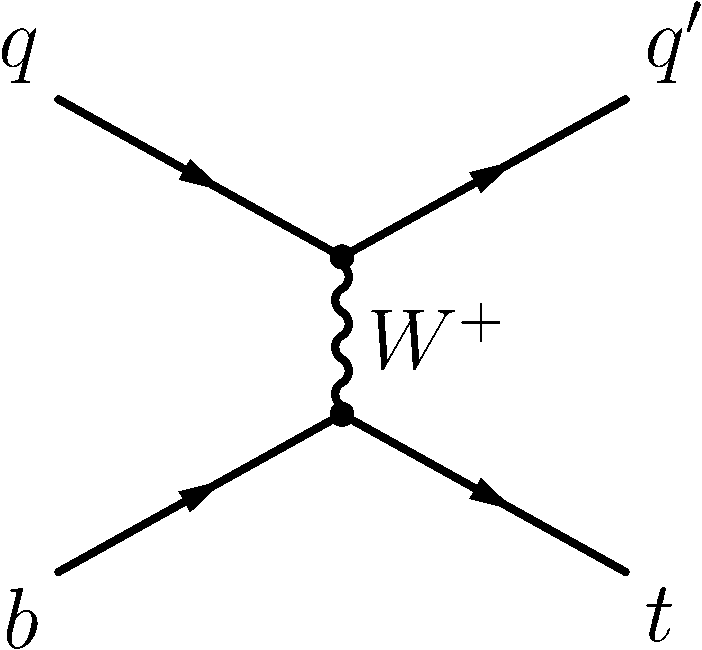
\includegraphics[width=0.18\textwidth]{figures/tchannel22}
		\hspace{0.5cm}}
		\subfigure[]{
	    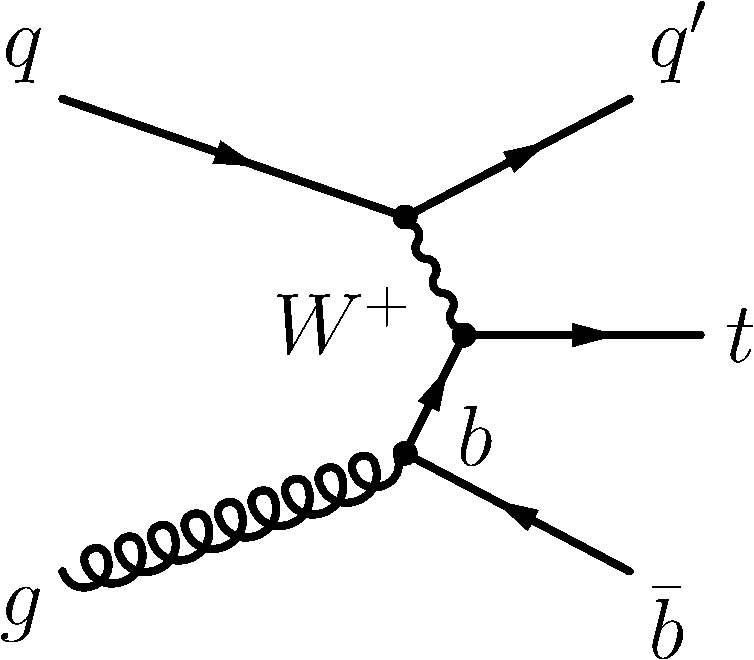
\includegraphics[width=0.18\textwidth]{figures/tchannel23}}
	    \hfill
	    \caption{\label{fig:FG}Leading order Feynman diagrams for single top quark production via the $t$-channel in the five flavour scheme (a) and in the four flavour scheme (b). The latter can also be seen as an NLO contribution in the four flavor scheme.}
	  \end{center}
	\end{figure}

The aim of the analysis described in this note is to measure the inclusive single-top quark $t$-channel production cross section.

In this note the $t$-channel is considered as signal process, while the $s$-channel and W-associated production are included among the background processes. 
The analysis strategy is similar to the one applied in Refs.~\cite{TOP-11-021,TOP-12-038}, where the precision measurements of $t$-channel single-top-quark cross section has been performed at 7 and 8 TeV respectively.

This measurement is based on the leptonic decay channel in which the W boson produced in the top-quark decay further decays producing a muon and one or more neutrinos (via $\tau$ lepton decay chains) in the final state.
%The branching ratio of the top quark with a muon in or electron the final state is $B(\mathrm{t}\to\mu\nu \mathrm{b})=0.1080$~\cite{pdg} for each.
The cascade decay $\mathrm{t}\to\tau\to\mu$ is considered as part of the signal.

The signal fraction is extracted using a maximum likelihood fit of the distribution of the absolute value 
of the pseudorapidity of the light jet stemming from the parton recoiling against the top quark, $\etalj$, 
which allows to discriminate between single top $t$-channel and its main background contributions.
The expected distributions of $\etalj$ are determined from either simulation or from data.

Control samples are defined in order to check the distributions of the variables used in the analysis for the main background sources, 
and an ad-hoc study is performed on the effect of pile up interactions on the analysis.

The note is organized as follows:
\begin{itemize}
\item Sec.~\ref{sec:samples} describes the data and samples of simulated events and the software framework used;
\item Sec.~\ref{sec:selection} describes the event selection and the method used for the reconstruction of the top quark, defining the main variables
used in the analysis;
%\item Sec.~\ref{sec:2J0T} describes the control region used to check our W$+$jets distributions and our QCD extraction procedure.
%\item Sec.~\ref{sec:3JNT} describes the control region used to check our top-antitop distributions.
\item Sec.~\ref{sec:muonEff} describes the determination of the muon trigger
  and ID efficiencies.
\item Sec.~\ref{sec:controlplots} describes the control regions to check the \wjets and \ttbar~backgrounds.
\item Sec.~\ref{sec:qcd} describes the data-driven modelling of the $\qcd$ background and the estimation of its contribution to the signal region.
\item Sec.~\ref{sec:WHFExtraction} describes the modelling of the $\wjets$ background;
\item Sec.~\ref{sec:xsection} presents the cross section extraction based on a template fit to \etalj;
\item Sec.~\ref{sec:syst} explains in details how the systematic uncertainties have been estimated; 
\item Sec.~\ref{sec:results} summarizes the results.
\end{itemize}


%{\bf Disclaimer:}
%Many of the numbers and plots in this document are based on studies on pseudodata. They will updated using real collision data as soon as sufficient statistics are available. All MC-based plots with pseudo data are normalized to the aimed at luminosity of $1\,\mathrm{fb}^{-1}$. Plots with real data include all currently available data, corresponding to an integrated luminosity of around $20\,\mathrm{pb}^{-1}$.

%\include{todolist}


\section{Samples}
\label{sec:samples}
This study is based on an integrated luminosity of \mylumi, known within \lumiunc %~\cite{lumi}. 
The list of data samples used in this study is summarized in Table~\ref{tab:data}. We make use of the Single Muon (SingleMu) Primary Dataset ~\cite{sd}. In each run we excluded the luminosity sections flagged as bad according to the validations performed by each Detector Performance Group (DPG) and Physics Object Group (POG). Technically, we implement this by the use of a so called JSON file~\cite{json}; for the present note the full run range considered in this analysis (runs \runrange) was covered with the files in Ref.~\cite{json2}.

Two different setups are used to generate simulated single top $t$-channel events: a\MCATNLO ~\cite{amcatnlo}, used as default generator, and \POWHEG~1.0~\cite{Re:2010bp,Alioli:2010xd,Alioli:2009je,Frixione:2007vw}, interfaced in either case to {\PYTHIA~8.180} ~\cite{Sjostrand:2006za} for parton showering. 
A similar setup with {\MADGRAPH} interfaced to \PYTHIA is used for the simulation of top-antitop pair production.
The single top quark production in association with a W boson is simulated with \POWHEG, while vector bosons produced in association with jets (\vjets), and double vector boson (diboson) production are amongst the backgrounds taken into consideration and have been
simulated with {\MADGRAPH}~\cite{madgraph} interfaced to \PYTHIA~8.180 for parton showering.
The \PYTHIA generator is used to simulate \QCD samples enriched with isolated muons or electrons.
The value of the top quark mass used in all simulated samples is $m_{\cPqt}=$172.5\GeV.



\begin{sidewaystable}[h!]
\caption{Data samples.~\cite{sd}.}
\label{tab:data}
\centering
\begin{tabular}{ |l|c|c|c| }
  \hline
  Dataset & Run range &  Integrated luminosity & tag used \\
  \hline
  \hline
\small{/SingleMuon/Run2015B-17Jul2015-v1/MINIAOD} & 251162-251562 & \multirow{ 2}{*}{$\mylumi$} & GT \\
\small{/SingleMuon/Run2015B-PromptReco-v1/MINIAOD} & 251585-251883 &  & GT \\
%\small{/SingleMuon/Run2015C-PromptReco-v1/MINIAOD} & 254833 & $\mylumi\,\invfb$ & GT \\
  \hline
\end{tabular}
\vspace{1cm}
\caption{Monte Carlo datasets used in this analysis. 
The samples are generated either inclusively or with a final state restricted to the leptonic mode,
including electrons, muons, and taus. Where no references are given, the cross sections come from 
the generator itself. For the samples restricted to specific decay channels the branching ratio (BR) is included in the cross section value quoted. The "RunIISpring15DR74-Asympt50ns\_MCRUN2\_74\_V9A" part in the name is the same for all samples and has been replaced by "...".} 
\label{tab:samples}
\centering
\begin{tabular}{|c||c|c|}
                        \hline
    			Process        & $\sigma(\cdot BR)[{\rm pb}]$  & Dataset name \\
    			\hline \hline
    			single top and antitop $(t)$ & 70.3 (leptons only) (NLO)~\cite{tchanxsec}  & \small{/ST\_t-channel\_4f\_leptonDecays\_13TeV-amcatnlo-pythia8\_TuneCUETP8M1/...-v1/}\\
    			single top $(\rm tW)$ &35.6 (NNLL)~\cite{Kidonakis:2012db} & \small{/ST\_tW\_top\_5f\_inclusiveDecays\_13TeV-powheg-pythia8\_TuneCUETP8M1/...-v1}\\
    			single anti-top $(\rm tW)$ &35.6 (NNLL)~\cite{Kidonakis:2012db} & \small{/ST\_tW\_antitop\_5f\_inclusiveDecays\_13TeV-powheg-pythia8\_TuneCUETP8M1/...-v2}\\
			\hline
    			$\ttbar$       & 831.76 (NLO)~\cite{tchanxsec} & \small{/TT\_TuneCUETP8M1\_13TeV-powheg-pythia8/...-v4/} \\ 
                ${\rm W}(\to \ell\nu)+$\,jets      &     61,526.7 (leptons only) (NLO) & \small{/WJetsToLNu\_TuneCUETP8M1\_13TeV-amcatnloFXFX-pythia8/...-v1/}\\
                ${\rm Z}/\gamma(\to \ell\ell)+$\,jets  (*)    &     6025.2 (NLO) & \small{/DYJetsToLL\_M-50\_TuneCUETP8M1\_13TeV-amcatnloFXFX-pythia8/...-v2}\\
			$\mu$-enriched QCD (**)                &240,680  (LO) & \small{/QCD\_Pt-20toInf\_MuEnrichedPt15\_TuneCUETP8M1\_13TeV\_pythia8/...-v2/}\\
			\hline
    		  	\end{tabular}

			\vskip 2ex

			\begin{tabular}{ll}
%			(*)  & NLO cross section for $W+Jets$ = 36257.2   & \\		
			(*)   & $m_{ll} > 50$ GeV \\
			(**) & $\hat{p}_T > 20$ GeV, $p^{\mu}_T > 15$ GeV \\
			\end{tabular}
			%\vskip 2ex
			%\begin{tabular}{ |c||c| }
    			%\hline
    			%Process        & $\sigma[pb]$ \\
    			%\hline \hline
			%$W$ total      & 31,314 (NNLO) \\
			%$Wb\bar b$     & 35.3 (LO) \\
			%$Wc\bar c$     & FIXME (LO) \\
			%$Z$ total      & 3,048 (NNLO) \\
			%$Zb\bar b$     & 67.3 (LO) \\
			%$Zc\bar c$     & FIXME (LO) \\
			%$Wc$           & 3,628 (NLO) \\
			%\hline
    		  	%\end{tabular}
		%\end{center}
			\end{sidewaystable}

  
   
\clearpage

Signal simulated datasets are normalized to the NLO cross section of:

\begin{eqnarray}
\label{eq:sigmatot}
 \sigmattop &=&  \xsectheotop \xsectheotopscale\,\textrm{(scale)} \xsectheotoppdf \,\textrm{(PDF)}\nonumber\\
 \sigmatantitop &=&  \xsectheoantitop \xsectheoantitopscale\, \textrm{(scale)} \xsectheoantitoppdf\,\textrm{(PDF)}\nonumber\\
 \sigmat &=&  \xsectheo \xsectheoscale\, \textrm{(scale)} \xsectheopdf \,\textrm{(PDF)}
\end{eqnarray}

evaluated in the five-flavor scheme within {\sc Hathor}\,v2.1~\cite{HATOR,tchanxsec}. 


Table~\ref{tab:samples} summarizes the Monte-Carlo samples for signal and backgrounds, and provides the number of events and cross section for each sample. 
All the cross sections have been taken from the references listed in Table~\ref{tab:samples} or, when no reference is given, from the generator itself.
The simulation of the full detector response is based on GEANT~4~\cite{geant}, and assumes realistic alignment and calibration, tuned on data.




%{\bf FIXME: INSERT PILEUP TREATMENT}
        

%This analysis is performed within the software releases \verb+CMSSW_7_2_X+, \verb+CMSSW_7_3_X+ and \verb+CMSSW_7_4_X+, while it uses the Physics Analysis Toolkit (PAT)~\cite{pat} as a starting point and Particle Flow algorithms for reconstruction of physics objects. The recommended sequence \verb+PF2PAT+ is run in order to obtain the standard objects in the selection. When running on data, Global Tag \verb+74X_dataRun2_Prompt_v0+ is used, when running on simulation, \verb+MCRUN2_74_V9A+ is used.


\section{Selection and reconstruction}
\label{sec:selection}
The final-state topology in the $t$-channel is characterized by the presence of  exactly one isolated muon and a b jet from the top quark decay, as well as a light-flavour jet produced in the forward region. The splitting of the gluon from the initial state produces a second b quark (Fig. ~\ref{fig:FG}) that recoils against the top quark. The b jet from gluon splitting has generally a softer $p_\mathrm{T}$ spectrum and a broader $|\eta|$ distribution compared to the one produced in top-quark decay, thus the acceptance for events with two b jets reconstructed in the final state is expected to be small. In fact we can anticipate that using the selection described in this section, the number of signal events with two b jets reconstructed in the detector is smaller than the number of events with just one b jet.
Here in the following, we describe the object definitions and selection criteria.


\subsection{Object definition}
\label{sec:objects}

In this Section the basic analysis objects are defined on which the event selection and the kinematic reconstruction are based.
The reconstruction of all objects is done through the PF algorithm~\cite{CMS-PAS-PFT-09-001}. 

 \subsubsection{Tight Muons}
 \label{sec:tight_muon}
 Reconstructed muons within the \texttt{HLT\char`_IsoMu20\char`_eta2p1} trigger acceptance range ($|\eta| < 2.1$) and with a transverse momentum $p_\mathrm{T} >$22~\GeV are selected. The baseline muon selection contains ``global muons'' and has to meet additional muon quality requirements referred to as ``tight muon ID'', which corresponds to a subset of the PF muons. 
 
 More specifically, muons must have $\chi^2/\mathrm{ndof}<10$ and at least one valid hit in the muon chambers, in order to suppress hadronic punch-through and muons from decays in flight. To guarantee a good $p_\mathrm{T}$  measurement, muon candidates are required to have more than 5 valid hits in the silicon tracker, out of which at least one in the pixel detector so as to further suppress muons from decays in flight. At least two segments must match the global muon object in the muon chambers, for suppress punch-through and accidental track-to-segment matches. Furthermore, the (absolute) transverse impact parameter must be smaller than 0.2~cm with respect to the center of the estimated beam spot position in order to suppress the background due to cosmic-ray muons, while the longitudinal distance of the muon track relative to the leading primary vertex\footnote{If more than one primary vertex is identified, the one with largest sum of the squared transverse momenta of associated tracks is taken.} must be less than 0.5~cm at the point of the closest approach.
 
 We define the ``particle flow (relative) isolation'' ($\PFrelIso$) with the so-called ``DeltaBeta'' correction as
 \begin{equation}
 \PFrelIso = \frac{ \pfChargedHadronIso + max((\pfPhotonIso + \pfNeutralHadronIso - \pfPU),0)}{p_T}~,
 \label{eq:pfreliso}
 \end{equation}
 where $\pfChargedHadronIso$, $\pfPhotonIso$, and $\pfNeutralHadronIso$ are the sum of the transverse energies deposited by stable particles like charged hadrons, photons and neutral hadrons respectively, in a cone of size $\Delta R = \sqrt{(\Delta\eta)^2+(\Delta\phi)^2} = 0.4$ around the muon direction; $\pfPU \equiv \Delta\beta \times \sumPUPt \equiv 0.5 \times \sumPUPt$ is the sum of transverse momenta of tracks associated to non-leading, i.e. pileup, vertices, used to estimate the contribution of neutral particles from pileup events by applying a multiplicative factor of 0.5 that takes into account the neutral-to-charged particles ratio expected from isospin invariance. Therefore, the $\Delta\beta$ factor maps the expected neutral contribution in the isolation cone from the observed PU charged contribution. Tight muons are accepted by the requirement $\PFrelIso < 0.06$, which is expected to select signal events with $\sim70\%$ efficiency ($85\%$ corresponds to a cut-value of 0.12, which was used in a former version of the analysis).
 
 Finally, the $\Delta R = \sqrt{\Delta\eta^2+\Delta\phi^2}$ distance must be greater than 0.3 from any jet passing the selection of Sec.~\ref{sec:jets}.
 
 
 
 \subsubsection{Loose Muons}
 
 For the purpose of vetoing events with additional charged leptons, the selection requirements for these additional leptons are loosened. Any event with a further muon, within the full muon acceptance range ($|\eta| < 2.5$), having $p_\mathrm{T} >$~10~\GeV, the ``global'' or the ``tracker muon'' flag (a muon that is reconstructed in the inner tracker and has one segment in the muon chambers) and lying within $\PFrelIso < 0.2$, is rejected. 
 
 
 \subsubsection{Loose Electrons}
 
 The loose electron candidate selection requires a ``GsfElectron'', i.e. electron reconstructed matching a track with the clusters in the calorimeters, with $E_\mathrm{T} > 20\,$\GeV, $|\eta| < 2.5$ and passing a selection chain made by 9 variables and optimized in a cut-based approach. Due to the presence of strong correlation between the  $\Delta\phi$ and $|1/E-1/p|$ (with E the supercluster energy and p the track momentum at the point of closest approach to the beam spot) variables, optimization has been achieved only for one of them, albeit making a reasonable cut for the other. The present analysis then makes use of the cut-based ``electron veto'' working point ($95\%$ signal efficiency) derived using the PHYS14 samples for the PU20bx25 scenario. In addition, the barrel-endcap transition region ($1.44<|\eta|<1.57$) is exluded. Any event with one or more electron candidates as defined above is rejected.
 
 
 \subsubsection{Jets}
 \label{sec:jets}
 
 Jets are reconstructed using the anti-$k_t$ clustering algorithm~\cite{Cacciari:2008gp} with a cone size of 0.4, using the PF algorithm (PF objects as input objects) and after rejecting charged hadrons that are associated to a pileup primary vertex (``slimmedJets''). These jets have standard multi-level (on PU and electronic noise, on $|\eta|$ and on $p_\mathrm{T} >$) jet energy corrections (JEC) applied (L1FastJet, L2, L3) and a $p_\mathrm{T}$ cut at $10\,$\GeV. Technically, we apply the \verb+Summer12+ corrections determined from simulation on both data and simulation.  For data we further apply residual corrections derived from data themselves~\footnote{Label \texttt{Spring10DataV2\_L2L3Residual\_AK5}}. The jet energy is scaled by a factor that describes the detector response depending on the transverse energy and the pseudo-rapidity of the jet~\cite{CMS-PAS-JME-10-003}. To reduce contamination from pileup events, charged particle candidates not associated to the main primary vertex are subtracted event by event. The energy of the jet is then corrected by the amount of energy deposited by neutral pile-up hadrons in the jet area.
 
 The analysis considers jets within $|\eta|<4.7$ whose calibrated transverse energy is greater than 40~\GeV
 and which pass a set of quality cuts (``JET ID'') which are specific of the algorithm used. 
 PF jets must have more than one constituent, neutral hadronic and neutral electro-magnetic energy fractions smaller than 99\%, while their muon fraction should be at most 80\%. In addition, if central, they must have non-zero charged hadronic energy fraction and charged particle multiplicity, whereas their charged electro-magnetic energy fractions must be smaller than 99\%.
 
 Once the jet has been selected according to the above criteria, it is further categorized using a b-tagging discriminator variable 
 in order to distingush between jets stemming from the hadronization of a b-quark or a light parton.

\subsubsection{b Tagging}

Several b-tagging, i.e. identification of jets originating from  b  quarks, algorithms are available in CMS. Some exploit the long B-hadrons lifetime, others their semi-leptonic decay modes and others use kinematic variables related to the high 
B-meson mass and hard b-quark fragmentation function. Details are provided elsewhere~\cite{CMS-PAS-BTV-10-001}. More specifically, b-tagging  algorithms  based  on  displaced  tracks (track counting taggers, jet probability tagger), the presence of ``secondary'' vertices (secondary vertex taggers) or soft leptons (soft lepton taggers) or on a combination of these (combined secondary vertex taggers).  The combined secondary vertex (CSV) taggers combine kinematic variables from displaced tracks and secondary vertices using multivariate analysis (MVA) techniques. Two different taggers are used.  The first makes use of a likelihood ratio (LR), while the second uses a neural network. 
%For this study we use the CSVv2 algorithm at the ``tight'' working point corresponding to a threshold set to 0.941 and a 0.1144\% DUSG mistag efficiency, recomeneded by the The b-tagging Physics Object Group (POG).
For this study we use the CSVv2 algorithm at the ``tight'' working point corresponding to a threshold set to 0.97 and a 0.1\% DUSG mistag efficiency, recomeneded by the The b-tagging Physics Object Group (POG).
%
%\subsubsubsection{pile-up rejection and control-sample specific cuts }
%
%
%After the above cuts are imposed and the jet has been classified according to the b-tagging algorithm, the events are assigned to a specific sample ( see also in the following  Sec-~\ref{sec:leptonjetcounting}). 
%
%Additional cuts are be imposed in the different control regions
%
%For jets failing the b-tagging requirement the root-mean-square radius of the particles with respect to the jet axis ($RMS$) is required to be smaller than 0.025, in order to reject jets from pileup. This requirement is found to improve the agreement of simulation with data in the control regions defined in Sec.~\ref{sec:control}. 
%
%%/An extra cut on the jet $p_T > 60$~\GeV is performed in the signal region in order before performing the fit to extract the inclusive cross section. 
%
%More details will also be given later in this note. 
%%Furthermore, jets of both kinds are ignored if they are within $\Delta R<0.1$ of a tight muon candidate (defined as in Sec.~\ref{sec:tight_muon} apart of course the $\Delta R(\mu,jets)>0.3$ requirement) or $\Delta R<0.3$ of a tight electron candidate (defined as in Sec.~\ref{sec:tight_electron} apart from the requirements on the number of missed hits and photon-conversion veto).
%
\subsubsection{Missing transverse energy}

Defined in an analogous way as PF-based jets, PF-based $\MET$ is the opposite of the vectorial sum of the transverse momenta of the identified PF particles. Data-driven corrections of energy offset are also applied to PF-based \MET. No explicit cut is applied on $\MET$ in this analysis.


\subsection{High level trigger selection}
\label{subsec:hlt}
The offline kinematic thresholds for the prompt muon are imposed by the trigger choice. Therefore a study is performed to evaluate the sensitivity for each trigger requirement. Different single-muon trigger paths are unprescaled for the run range of the analysis of which three are compatible with our kinematics of interest. The \verb+HLT_IsoMu17_eta2p1+ path, imposing $|\eta|<2.1$ on the prompt muon, is the one with the lowest online muon \pt threshold. Other paths are \verb+HLT_IsoMu20_eta2p1+ and \verb+HLT_IsoMu20+ which differ in $\eta$ restriction.

The event selection for this study is exactly the same as that of the signal region, requiring the presence of exactly one prompt muon without any additional loose lepton, two jets of which only one is b-tagged, a W transverse mass above 50 GeV and a top quark candidate with the mass falling in $[130,225]\,\GeV$. The prompt muon selection criteria changes according to the trigger choice. Table~\ref{tab:trigMuSel} summarize the online muon selection with the corresponding offline conditions. The last row is a mixture of the 17 GeV trigger and non-restricted 24 GeV path where a lower offline \pt threshold is applied in $|\eta|<2.1$.

 \begin{table}[t!] 
 \caption{Online muon selection requirements and the corresponding offline conditions}
  \label{tab:trigMuSel}
 \begin{center}
\begin{tabular}{|c|c|}
\hline
Online 	& Offline\\
\hline
\small{HLT\_IsoMu17\_eta2p1 (I)}	& $|\eta|<2.1 ,\, \pt>20\,\GeV$	\\
\small{HLT\_IsoMu20 (II)}			& $|\eta|<2.4 ,\, \pt>22\,\GeV$	\\
\small{HLT\_IsoMu20\_eta2p1} 		& $|\eta|<2.1 ,\, \pt>22\,\GeV$ \\
\small{(I) or (II)}					& $(\pt>20\,\GeV,\,|\eta|<2.1)$ \& $(\pt>22\,\GeV,\,2.1<|\eta|<2.4)$\\
\hline
\end{tabular}
\end{center}
\end{table}

The selection is applied on $t$-channel signal and QCD multijets and $S/\sqrt{B+(\Delta B)^2}$ is taken as a measure for the sensitivity. Table~\ref{tab:hltSensitivity} shows this measure and the yields for different scenarios. The selection corresponding to \verb+HLT_IsoMu20_eta2p1+ seems to have the best performance although the differences are not very significant.

 \begin{table}[t!] 
 \caption{Expected yields and sensitivities at $\mylumi$ for QCD and the $t$-channel signal using different online and offline muon selections. }
  \label{tab:hltSensitivity}
 \begin{center}
\begin{tabular}{|c|c|c|c|}
\hline
Scenario 	& $t$-channel&QCD&$S/\sqrt{B+(\Delta B)^2}$\\
\hline
\small{HLT\_IsoMu17\_eta2p1 (I)}	& $36.6\pm0.99$	&$29.6\pm5.91$	&4.56\\
\small{HLT\_IsoMu20 (II)}			& $35.2\pm0.97$	&$27.2\pm5.67$	&4.57\\
\small{HLT\_IsoMu20\_eta2p1} 		& $36.8\pm0.99$	&$28.4\pm5.79$ 	&4.67\\
\small{(I) or (II)}					& $38.2\pm1.0$	&$30.7\pm6.03$	&4.66\\
\hline
\end{tabular}
\end{center}
\end{table}

Efficiencies for this trigger in data and simulation are obtained using a ``Tag and Probe'' method and details are given in Section \ref{subsec:hlt}. 
%The corresponding data-to-MC correction factors are provided in bins of muon $\pt$, Table~\ref{tab:hltsf}.

% \begin{table}[t!] 
% \caption{The data-to-MC correction factors in bins of muon $\pt$ for the HLT\_IsoMu20\_eta2p1 trigger path.}
%  \label{tab:hltsf}
% \begin{center}
%\begin{tabular}{|l|c|c|c|c|c|}
%\hline
%Bins in muon $\pt$ 	& & & & & \\
%\hline
%Scale factor		& & & & & \\
%\hline
%\end{tabular}
%\end{center}
%\end{table}



\subsection{Lepton counting}
\label{sec:leptoncounting}

As previously described in Sec.~\ref{sec:objects}, we require the presence of exactly one tight muon.
In order to reduce the contribution of dilepton events, which can come from $\ttbar$ or from Drell--Yan processes, 
we veto events with additional loose muons or loose electrons.


\subsection{Jet and b-jet counting}
\label{sec:bcounting}

The signature of the $t$-channel single-top production includes 3 partons in the final state, see Fig.~\ref{fig:FG}(b): 
one light quark recoiling against the virtual W boson, one b quark from the 
top-quark decay, and a second b quark from the initial gluon splitting. 
The second b quark has a softer \pt and a harder $\eta$ spectrum with respect to the one coming from the top-quark decay.
As a result, jets stemming from the hadronization of the latter are less likely to be selected due to the \pt cut on the jet, and if selected they are less likely to be tagged, due to the intrinsic limit on the acceptance in $\eta$ of the b-tagging algorithm, which is limited to the tracker acceptance ($|\eta|<2.5$). For that reason the region with two jets, with one of them being tagged as b jet, provides the largest fraction of signal events. In order to test the modelling of the main background processes it is useful to define further regions, which are enriched in certain background processes. For that purpose we use the notation "nJmT" or the wording "n-jets, m-tags" to refer to a sample that has exactly n reconstructed jets, exactly m of which pass the b tag threshold. Notable samples which are studied and used in this analysis are the 2J0T sample (enriched in \wjets), the 2J1T sample (signal region with the largest signal fraction among all regions), and the 3J2T region (enriched in \ttbar).

%%
%%	\begin{figure}[h]
%%	  \begin{center}
%%            \subfigure[]{
%%            \includegraphics[width=0.48\textwidth]{figures/selection/NBTags_VLightVSTChan_Muons.pdf}} 
%%	    \caption{\label{fig:btag}{	Number of tags with $D_{TCHP} > 3.41$ for data and simulation for signal and \wjets normalized to the same area, after the 2 jets request.  }}
%%	  \end{center}
%%	\end{figure}
%%%Hence we expect most signal events to have only one b-tagged jet. 
%%%&	The highest discriminator value of the high-purity track-counting $b$ tagger in the event is shown in Fig.~\ref{fig:btag}(a), and 
%The b-tag multiplicity in 2-jets events is shown in Fig.~\ref{fig:btag}(a) and~\ref{fig:btag}(c) for data and simulation, 
%and in Fig.~\ref{fig:btag}(b) and ~\ref{fig:btag}(d)
%for signal and W+lf.
%The contribution of processes without b quarks in the final state is strongly suppressed in the 1-tag sub-sample, 
%showing the largest population of signal events at the same time; the small 2-tags sub-sample is dominated by $\ttbar$. 
%Therefore, selected events are required to have exactly one b-tagged jet. 
%%%	\begin{figure}[h]
%%%	  \begin{center}
%%%            \subfigure[]{
%%%            \includegraphics[width=0.48\textwidth]{figures/NBTags_Muons.pdf}}
%%%	    \subfigure[]{
%%%	    \includegraphics[width=0.48\textwidth]{figures/NBTags_Electrons.pdf}}
%%%	    \subfigure[]{
%%%	    \includegraphics[width=0.48\textwidth]{figures/NBTags_VLightVSTChan_Electrons.pdf}}
%%%	    \hfill
%%
%%
%Figure~\ref{fig:nbjetPresel} shows the jet multiplicity after selecting exactly 1 and 2 b-tagged jets, comparing data and MC.
%%
%%Figure~\ref{fig:nbjetPresel} shows the jet multiplicity after selecting exactly 1 and 2 b-tagged jets, comparing data and MC.

%%
%%	\begin{figure}[h]
%%	  \begin{center}
%%	    \subfigure[]{
%%	    \includegraphics[width=0.48\textwidth]{figures/selection/NJetsnJNoPU1TMuStack.pdf}} 
%%	    \subfigure[]{
%%	    \includegraphics[width=0.48\textwidth]{figures/selection/NJetsnJNoPU2TMuStack.pdf}} 
%%%	    \subfigure[]{
%%%            \includegraphics[width=0.48\textwidth]{figures/general/nJEleStack.pdf}}
%%%            \subfigure[]{
%%%            \includegraphics[width=0.48\textwidth]{figures/NJets_TTBarVSTChan_Electrons.pdf}}
%%	    \caption{\label{fig:nbjetPresel}{Jet multiplicity after the lepton counting in data and simulation requiring exactly 1 (a) and 2 (b) jets passing the trackcounting high purity tight threshold.}}
%%	  \end{center}
%%	\end{figure}
%%


\subsection{Transverse W boson mass}
To further suppress contributions from processes where the muon does not come from a leptonically decaying W boson, 
a selection based the reconstructed transverse W-boson mass $\mTW$ is made. The transverse W-boson mass is defined as:  

\begin{equation}
  \mTW = \sqrt{\left(p_{T,l} + p_{T,\nu}\right)^2 
    - \left( p_{x,l} + p_{x,\nu} \right)^2 
    - \left(  p_{y,l} + p_{y,\nu} \right)^2}~,
  \label{eqn:mTW}
\end{equation}
where the transverse momentum components of the neutrino are approximated by the components of the missing transverse energy vector, $\vec\MET$.
Only events with $\mTW > 50\,$\GeV are kept for the analysis.

%
%This variables is used for \qcd rejection in the muon channel. More details on the \qcd treatment can be found in section ~\ref{sec:QCD}
%
%
%%Figure~\ref{fig:mTW} shows the distribution of the $\mTW$ distribution after the preceding selection. 
%%In Fig.~\ref{fig:mTW} the QCD background can be nicely distinguished, since the transverse mass of the alleged W bosons accumulates 
%%at low values while all processes with real W bosons tend to cluster around the W mass
%%(this feature is known in the literature as ``Jacobian peak''). 
%%	Hence, the reconstructed transverse $W$-boson mass is required to be above 50~\GeV for the event to be kept. 
%%
%%
%%	\begin{figure}[h]
%%	  \begin{center}
%%	    \subfigure[]{
%%	      \includegraphics[width=0.48\textwidth]{figures/2j1t/mtwMassMuStack.pdf}}
%%	    \subfigure[]{
%%	      \includegraphics[width=0.48\textwidth]{figures/MTWMass_QCDvsTChan_Muons.pdf}} \\
%%            \subfigure[]{
%%              \includegraphics[width=0.48\textwidth]{figures/2j1t/metPtEleStack.pdf}}
%%           \subfigure[]{
%%              \includegraphics[width=0.48\textwidth]{figures/MET_QCDvsTChan_Electrons.pdf}}
%%            \caption{\label{fig:mTW}{Transverse mass after the entire selection minus the $\mTW$ ($\MET$) cut, 
%%                in data and simulation (a: muons, c: electrons) and for signal and QCD background (b: muons, d: electrons). }}
%%	  \end{center}
%%	\end{figure}	
%%
%%	\begin{figure}[h]
%%	  \begin{center}
%%	    \subfigure[]{
%%	      \includegraphics[width=0.48\textwidth]{figures/mtwMass_WSample_noSyst_MuStack.pdf}}
%%	    \subfigure[]{FIXME
%%	      \includegraphics7~[width=0.3\textwidth]{CMScol}}
%%           \subfigure[]{
%%             \includegraphics[,width=0.48\textwidth]{figures/mtwMass_WSample_noSyst_EleStack.pdf}}
%%	    \subfigure[]{FIXME
%%	      
\includegraphics[width=0.3\textwidth]{CMScol}}
%%          \caption{\label{fig:mTW_nobtag}{Transverse mass after the entire selection minus the $M_T$ in the zero $tche$ tag bin, corresponding to Sample A defined in ~\ref{sec:wjets} (a muons, b electrons).}}%FIXME, and optimization of the threshold (b muons, d electrons).}}
%%	  \end{center}
%%	\end{figure}	
%%
%%, its better stability against variations of the \MET~scale (see Sec.~\ref{sec:syst}), and because \MET~turns out to be quite correlated with muon momentum and muon isolation in our QCD sample, since most of the surviving QCD events in the muon channel, and many also in the electron channel, have a true lepton coming from $b$ or $c$ decay, therefore they also have a true neutrino.
%%Moreover, differently from \MET, the $M_T$ distribution is roughly similar for all non-QCD events, and this permits a very simple way to extract the amount of QCD background from data, as presented in Sec.~\ref{sec:qcd}.
%%In this analysis the $\mTW$ threshold is determined for muons with the following procedure:  
%%a fit to the $\mTW$ distribution is performed as described in Sec.~\ref{sec:qcd} in order to obtain the number of W-like and QCD-like events in the data sample. 
%%The $\mTW$ threshold is then selected maximizing the figure of merit $W/\sqrt{W+Q+(kQ)^2}$, with $k=50\%$, where $W$ ($Q$) is the estimated number of W-like 
%%(QCD-like) events, and which takes into account the total uncertainty on the number of QCD-like events determined in the fit. %More details are given in Appendix~\ref{sec:mt_cut}.
%%The threshold chosen for muons is $\mTW>40$~\GeV , while for electrons it is $\MET>35$~GeV.  
%%
%
%\subsection{\etalj}
%\label{sec:etalj}
%
%
%The distribution of the pseudorapidity $\etalj$  of the recoil from the fragmentation of
%a light quark in the $t$-channel scattering (Fig.~\ref{fig:FG}(c)) extends to value larger than for the background 
%processes, as shown in Fig.~\ref{fig:etalj_mc}.
%
%\begin{figure}[htp]
%\centering
%\includegraphics[angle=00,width=0.48\textwidth]{figures/tChanTTEta.pdf}
%\caption{Pseudorapidity of the untagged jet (\etalj) for the signal after requiring 2 jets 1 tag vs the distribution of the same variable for 
%\tt events, normalized to unity }
%\label{fig:etalj_mc}
%\end{figure}
%
\subsection{Top quark reconstruction}
\label{sec:topreco}

In order to define signal and sideband regions based on the top quark mass and to analyze the kinematics of singly produced top quarks, the fourvector of the top quarks have to be reconstructed from the decay products. All top-quark decay products are reconstructed in the detector, except for the neutrino which escapes unobserved. While the transverse momentum of the neutrino can be inferred from the missing transverse energy, its longitudinal momentum has to be derived based on  extra assumptions. Once the leptonically decaying W boson is reconstructed the selected jets have to be assigned to the final state quarks in the top quark decay chain.

\subsubsection{W-boson reconstruction}
\label{mlbnu}

The first step in the reconstruction of the top quark from its decay products is the reconstruction of the W boson. 
We assume that the $x$ and $y$ components of the missing transverse energy are entirely due to the escaping neutrino, 
and apply the W-mass constraint in order to extract the unknown $z$ component ($p_{z,\nu}$):
\begin{equation}
\label{eq:wconstraint}
\mW^2 = (E_{\ell} + \sqrt{{\MET}^2 + p_{z,\nu}^2})^2 - (\vec p_{T,\ell}+\vec\MET)^2 - (p_{z,\ell}+p_{z,\nu})^2 ~.
\end{equation}

This equation has in general two solutions:
\begin{equation}
\label{eq:solutions}
p_{z,\nu} = \frac{\Lambda \cdot p_{z,\ell}}{p_{T,\ell}^2} 
\pm \sqrt{
\frac{\Lambda^2\cdot p^2_{z,\ell}}{p_{T,\ell}^4} 
- \frac{E^2_{\ell}\cdot {\MET}^2 - \Lambda^2}{p_{T,\ell}^2}
}~,
\end{equation}
with
\begin{equation}
\label{eq:muW}
\Lambda = \frac{\mW^2}{2} + \vec p_{T,\ell}\cdot \vec \MET~.
\end{equation}

In the case of two real solutions for $p_{z,\nu}$ (in $65\%$ of all cases), different choice criteria have been proposed~\cite{Abazov:2009ii, Aaltonen:2009jj}. The solution with the smallest absolute value is chosen in the present analysis. By looking at truth information in simulated events it is found that, in $63.4\%$ of the selected events with real solutions, the smallest $|p_{z,\nu}|$ solution is closer to the true neutrino $p_{z}$ than the other solution. Figure~\ref{fig:pz_solution} shows the diffence in $p_z$ of the reconstructed neutrino with respect to the true neutrino for the cases of choosing the $\min |p_z|$ value, the $\max |p_z|$ value and the closest value amongst the two solutions ($\min \Delta p_{z}$).

\begin{figure}[hbpt]
\begin{center}
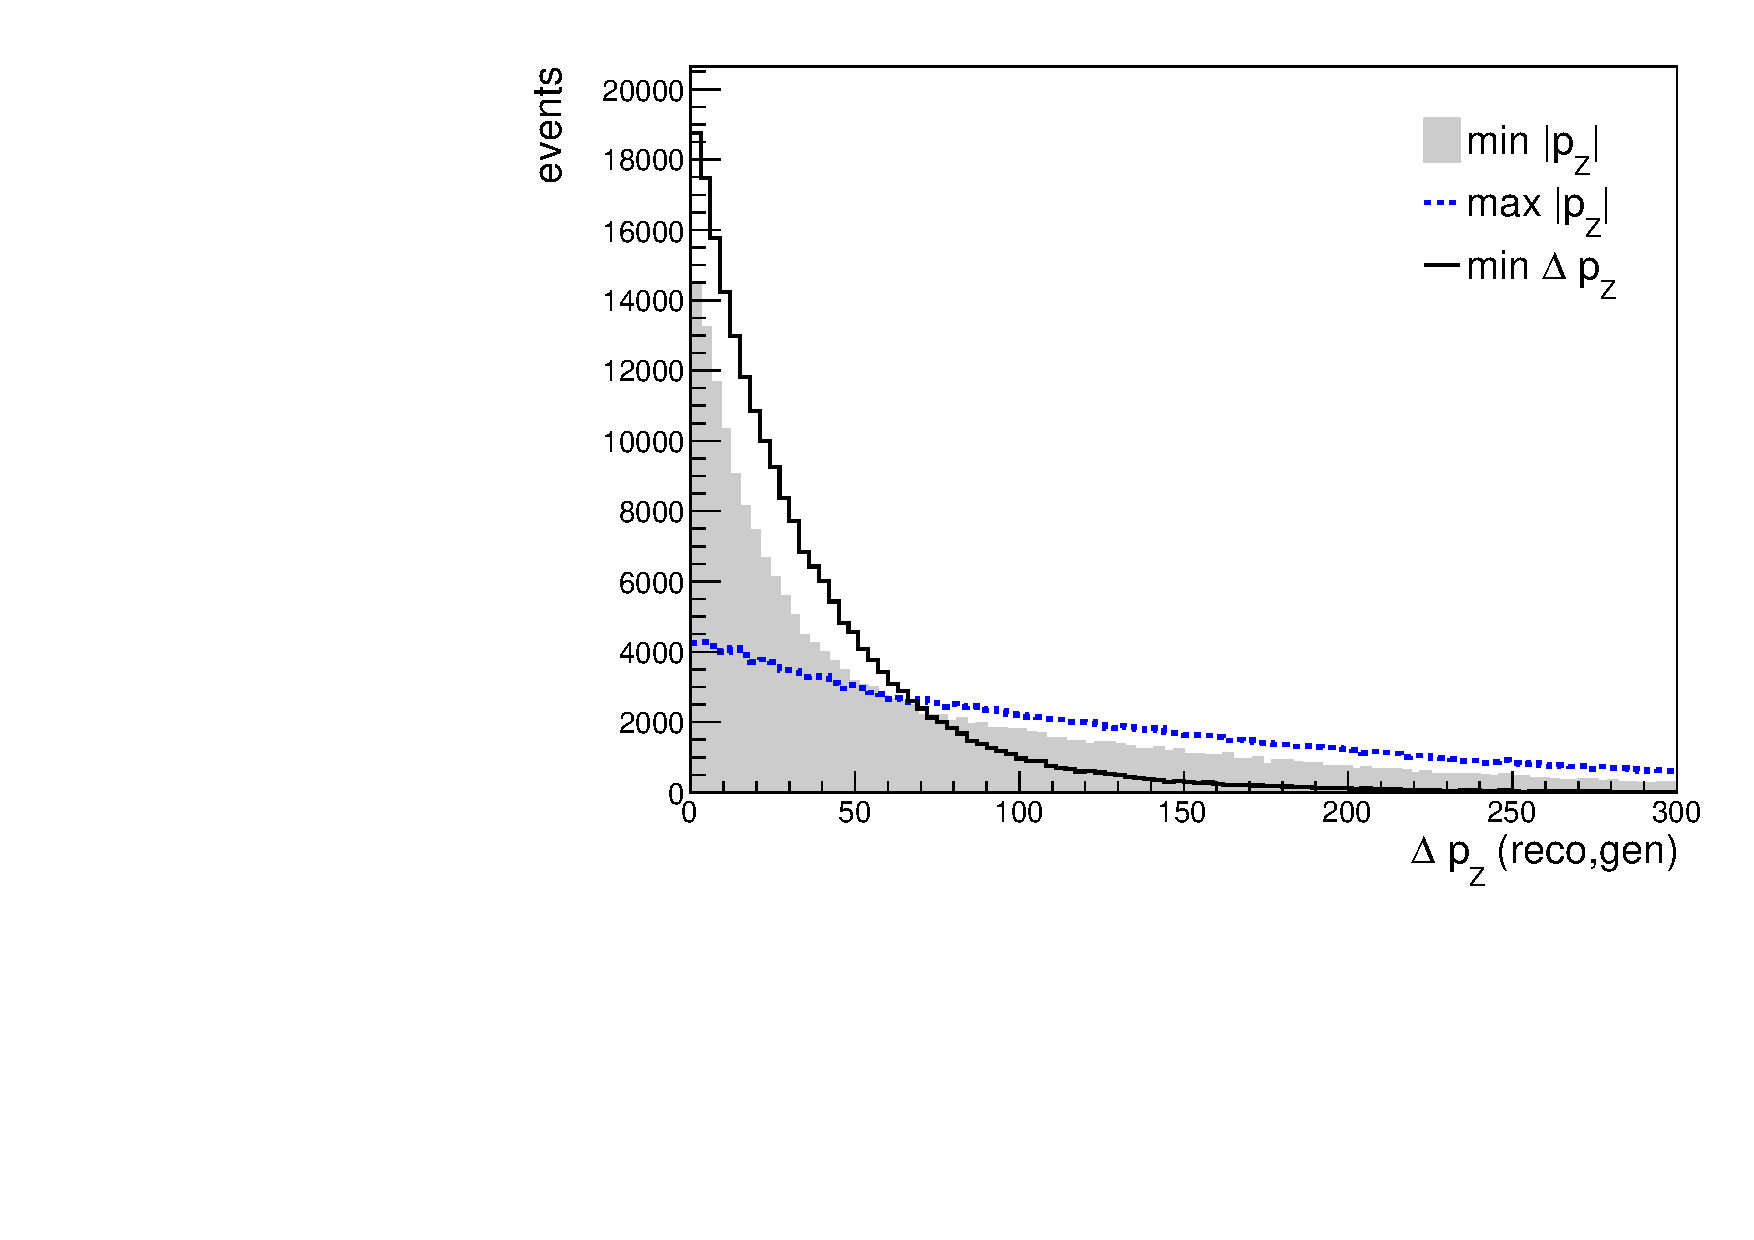
\includegraphics[width=0.6\textwidth]{figures/pz_solution.pdf}
\caption{\label{fig:pz_solution}Comparison of $p_{z}$-solutions against the difference in $p_{z}$ to the true neutrino.}
\end{center}
\end{figure}

If the discriminant in Eq.~(\ref{eq:solutions}) becomes negative, or equivalently $\mTW$ is larger than $\mW$, 
the solutions have an imaginary component. 
This happens in 35\% of the cases, mostly due the finite $\MET$ resolution. Lepton momentum resolution and the finite W intrinsic width give negligible contributions.
Several schemes have been used to deal with this situation~\cite{Abazov:2009ii, Aaltonen:2009jj}. In this analysis the imaginary component is eliminated by modifying $\MET$ such to give $\mTW = \mW$, still respecting the $\mW$ constraing from Eq.~(\ref{eq:wconstraint}). This is obtained by imposing that the discriminator, and thus the square-root term in Eq.~(\ref{eq:solutions}), are null. This condition gives a quadratic relation between 
$p_{x,\nu}$ and $p_{y,\nu}$, with two possible solutions, 
among which the one with minimal distance between $p_{T,\nu}$ and $\MET$ is chosen.


\subsubsection{Jet-parton assignment}

\begin{figure}[hbpt]
\begin{center}
\subfloat[][]{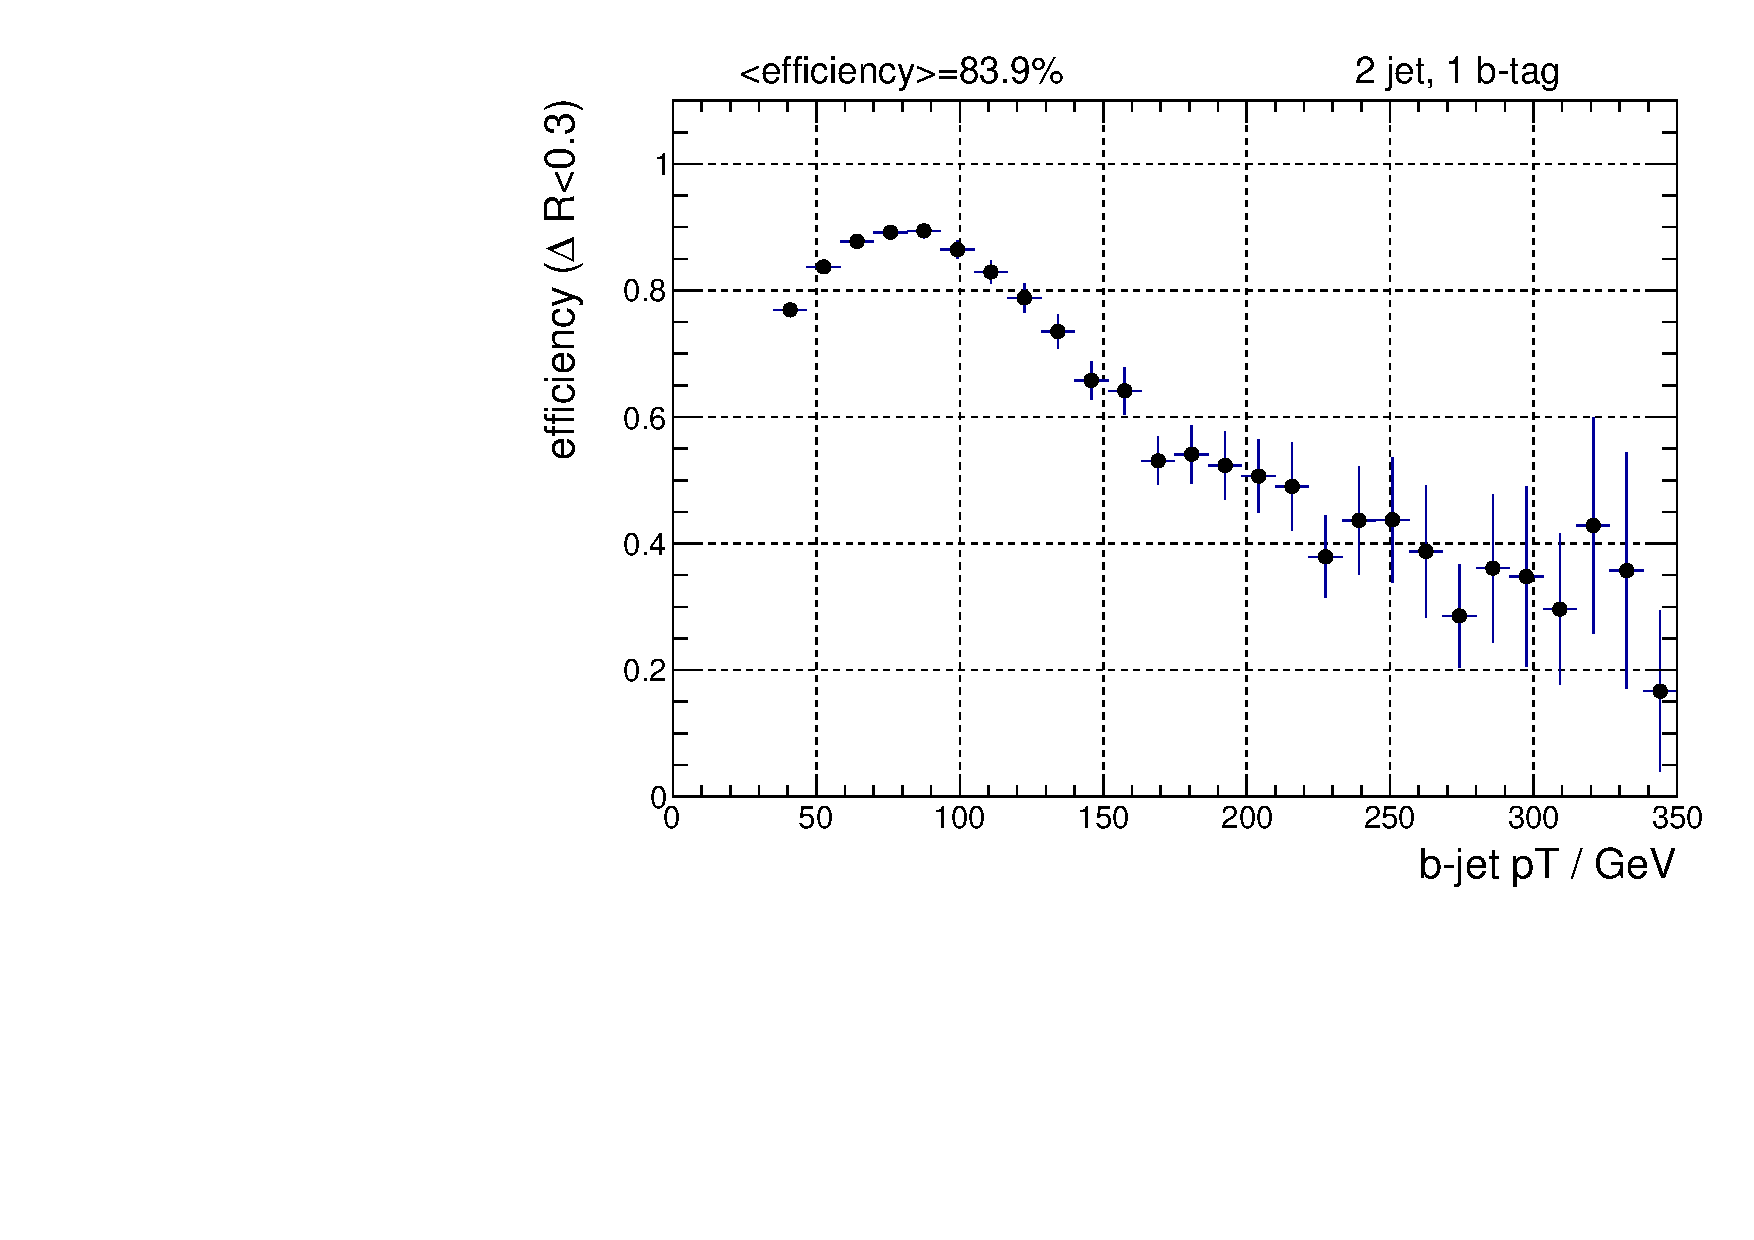
\includegraphics[width=0.45\textwidth]{figures/reconstruction/matching_topdecay_2j1t_pt.pdf}}\hspace{0.05\textwidth}\subfloat[][]{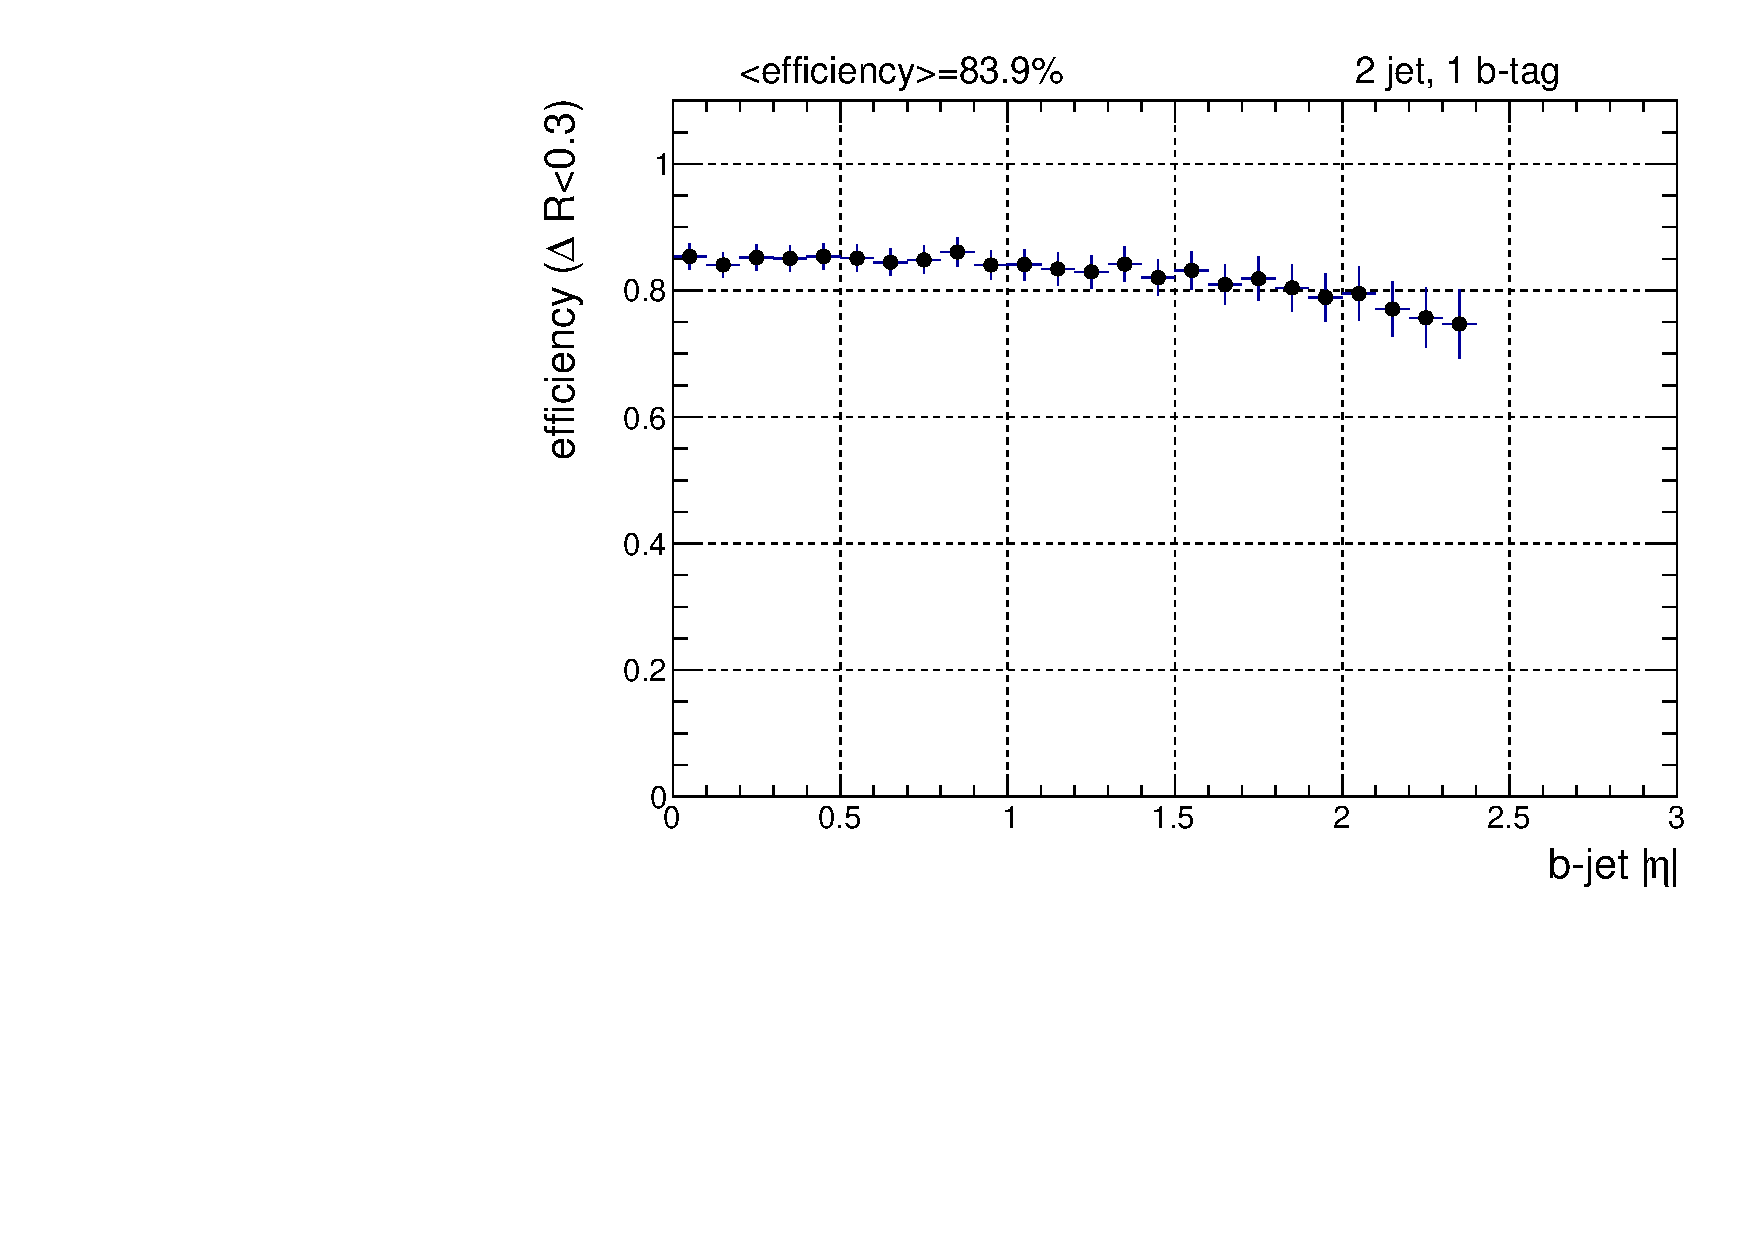
\includegraphics[width=0.45\textwidth]{figures/reconstruction/matching_topdecay_2j1t_eta.pdf}}
\caption{\label{fig:2j1t_matching_bjet_topdecay}Matching efficiencies between the true b-quark from the top decay and the selected tagged jet ($\Delta R<0.3$) in the ``2jet 1tag'' signal region.}
\end{center}
\end{figure}

In the second step the selected jets have to be assigned to the final state quarks from the top-quark decay. In the 2J1T region the procedure is straight forward: the tagged jet is assigned to the b-quark from the top-quark decay, the non-tagged jet is assigned to the light quark. The b-tagged jet matches the true b quark  from top-quark decay in simulated events in about 83.9\% of the selected signal events, using as matching criterion a distance of $\Delta R < 0.3$ between the jet and the parton. The fraction of events with wrong assignmet are events in which the selected b-tagged jet stems from the second b-quark from the initial gluon splitting and not from the decay of the top quark. Figure~\ref{fig:2j1t_matching_bjet_topdecay} shows the matching efficiencies against the transverse momentum and pseudorapidity of the selected jet.


\begin{figure}[hbpt]
\begin{center}
\subfloat[][]{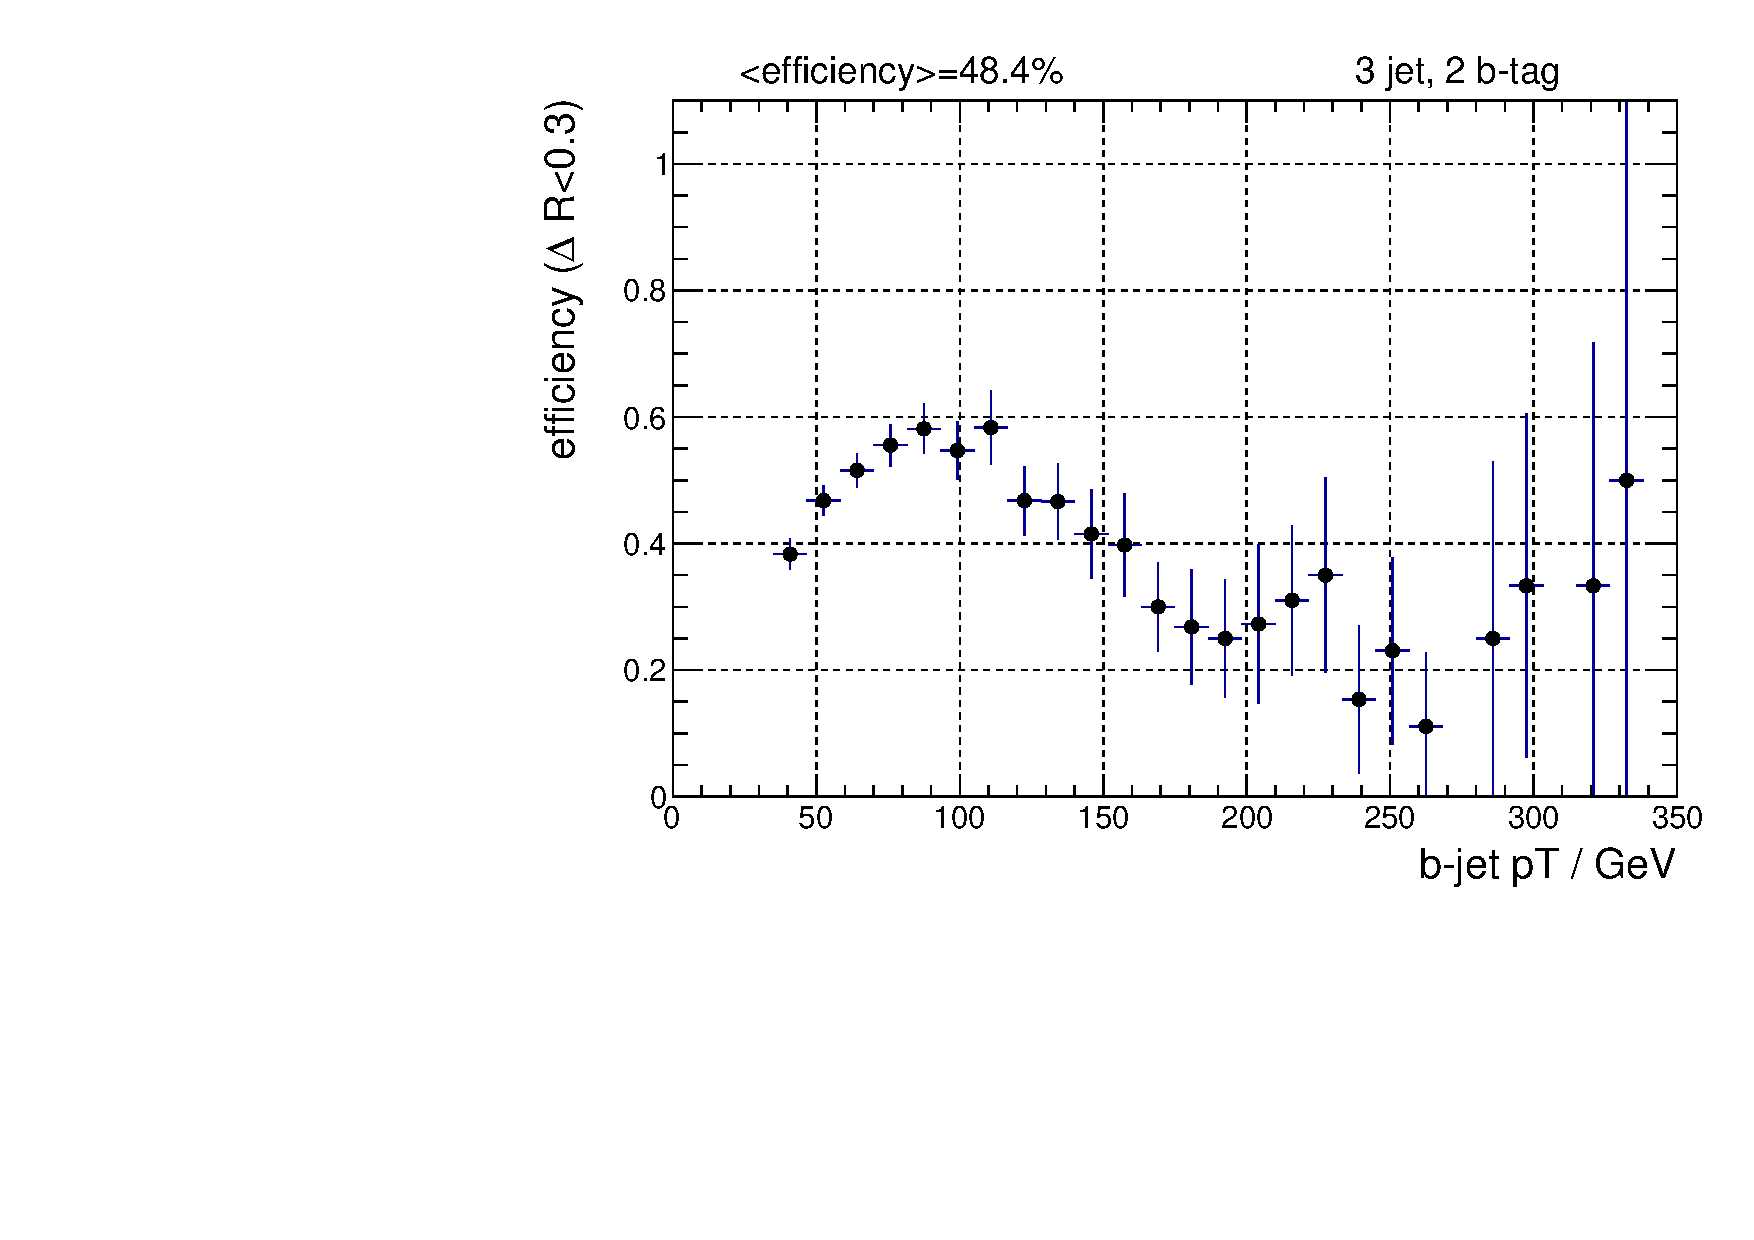
\includegraphics[width=0.45\textwidth]{figures/reconstruction/matching_topdecay_3j2t_pt.pdf}}\hspace{0.05\textwidth}\subfloat[][]{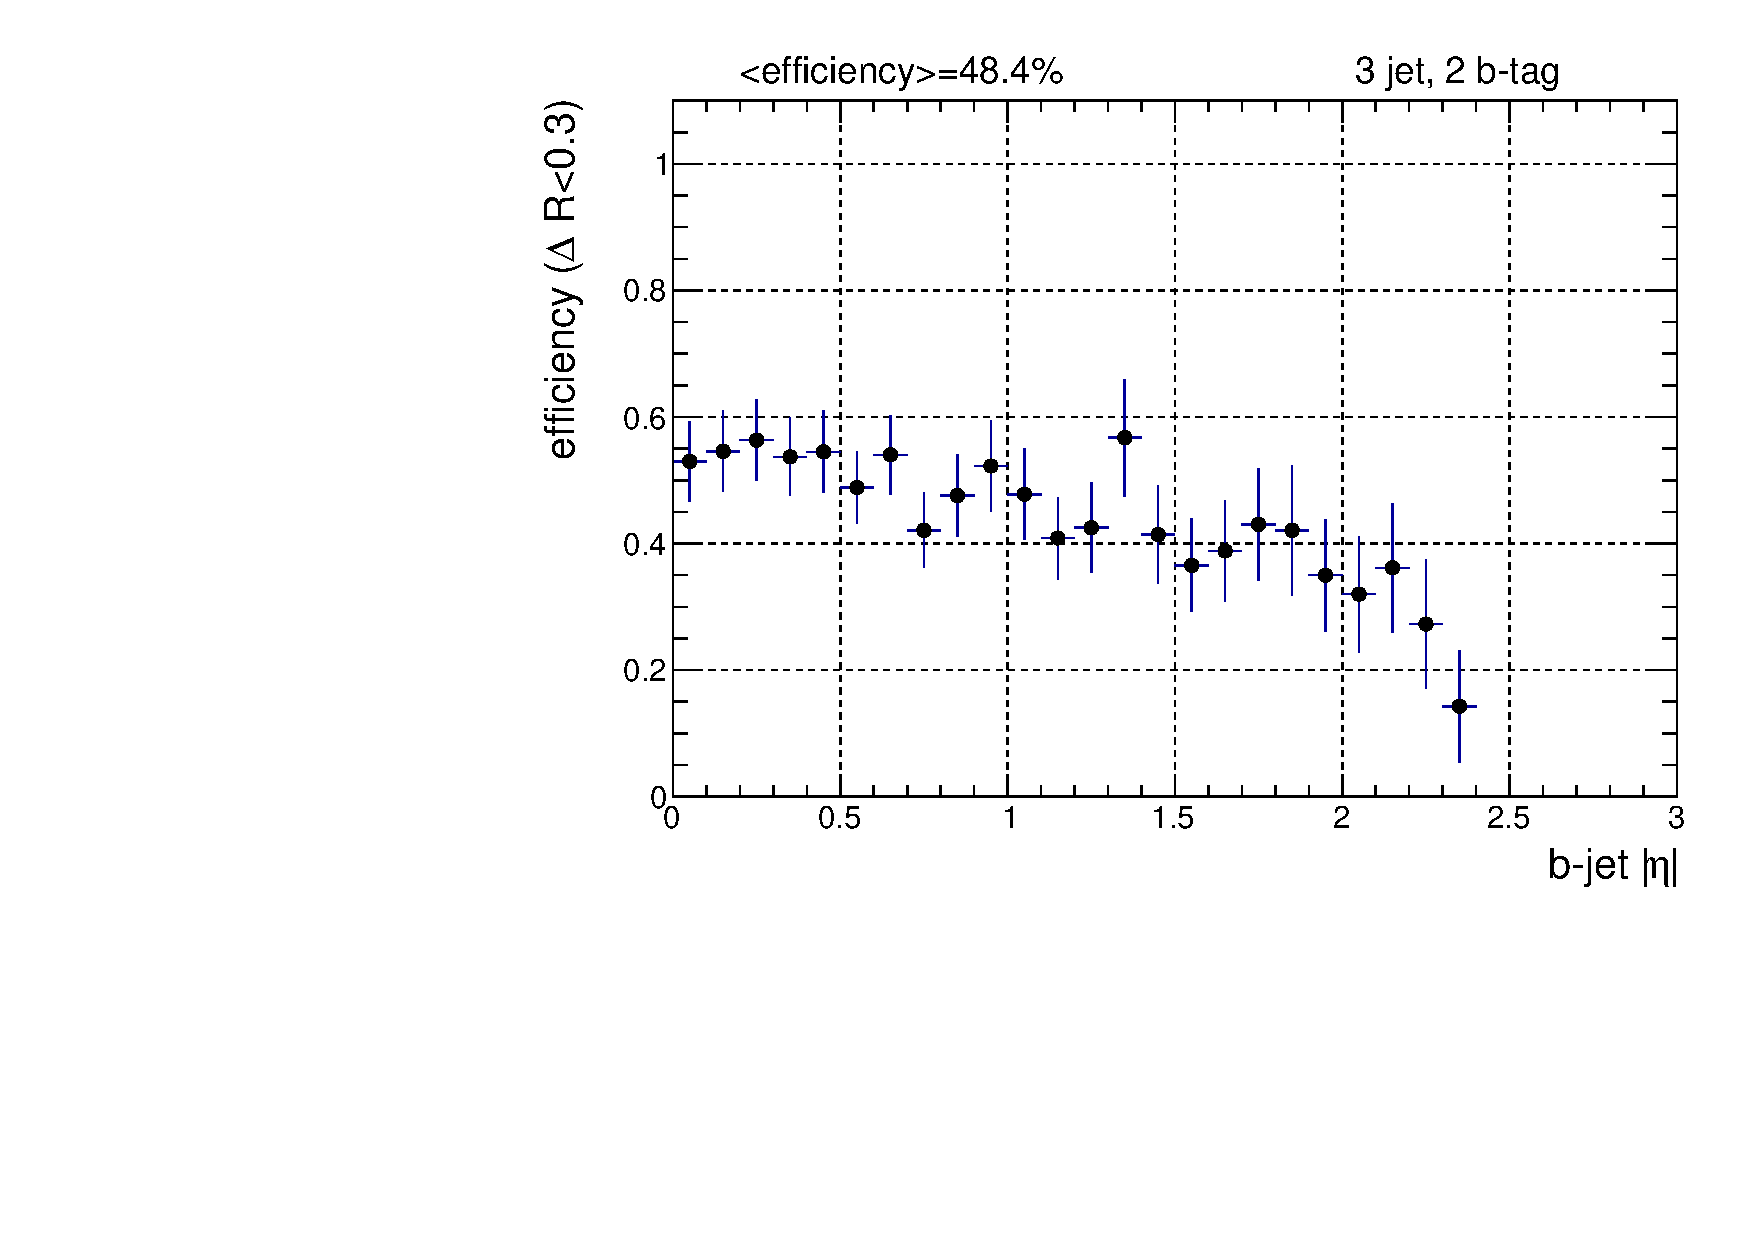
\includegraphics[width=0.45\textwidth]{figures/reconstruction/matching_topdecay_3j2t_eta.pdf}}
\caption{\label{fig:3j2t_matching_bjet_topdecay}Matching efficiencies between the true b-quark from the top decay and the selected tagged jet ($\Delta R<0.3$) in the ``3jet 2tag'' control region.}
\end{center}
\end{figure}


In the 3J2T region the non-tagged jet is again assigned to the light quark. From the two tagged jets the one with the larger value of the b-tag discriminator is assigned to the b quark from the top-quark decay, while the other tagged jet is assigned to the second b quark from the gluon splitting. This choice is correct in 48.4\% of all cases, estimated on simulated signal events using the same matching criterion as described above. The matching efficiencies against the transverse momentum and pseudorapidity of the selected jet are displayed in Fig.~\ref{fig:3j2t_matching_bjet_topdecay}.

          
                
\subsection{Top quark mass cut}

In the signal region (2J1T) we apply an additional cut on the invariant mass of the reconstructed top quark. Events inside the mass window between $130\,$\GeV and $225\,$\GeV are kept while the events outside this region are used to model the background from $\wjets$ (see Sec.~\ref{sec:WHFExtraction}).


\subsection{Event yields}
                
Table~\ref{tab:yields} summarizes the data yield surviving each selection step applied in the current analysis in the signal region 2J1T along with the yields for the signal and various background processes, obtained from MC simulation and scaled to an integrated luminosity of \mylumi. An illustration of table~\ref{tab:yields} is provided in Fig.~\ref{fig:cutflow}.            

\begin{table}[H!] 
 \caption{The number of data events passing each selection step. For comparison also the numbers for the signal and different BG processes are given, obtained from MC simulation and scaled to an integrated luminosity of \mylumi.}
  \label{tab:yields}
 \begin{center}
\begin{tabular}{l|c|c|c|c|c|c|c}
- & QCD & W/Z+Jets &\tt~ and tW & $t$-channel & Sum & Data & Data/MC\\
\hline
Trigger & $3.5\times10^5$ & $4\times10^5$ & 5218 & 616 & $7.5\times10^5$ & 610452 & $79\%$\\
== 1 $\mu$ & $5\times10^4$ & $3\times10^5$ & 3398 & 481 & $3.5\times10^5$ & 318252 & $90\%$\\
== 2 Jets & 2061 & 7962 & 963 & 167 & 11153$\pm$81 & 9509 & $85\%$\\
== 1-bJet & 209 & 127 & 335 & 58 & 729$\pm$18 & 595 & $82\%$\\
$m_T > 50$ & 61 & 88 & 229 & 40 & 418$\pm$11 & 379 & $91\%$\\
$m_{\ell\nu b}$ & 38 & 40 & 157 & 33 & 268$\pm$8 & 252 & $94\%$\\
\end{tabular}
\end{center}
\end{table}


\begin{figure}[H!]
\begin{center}
\subfloat[][]{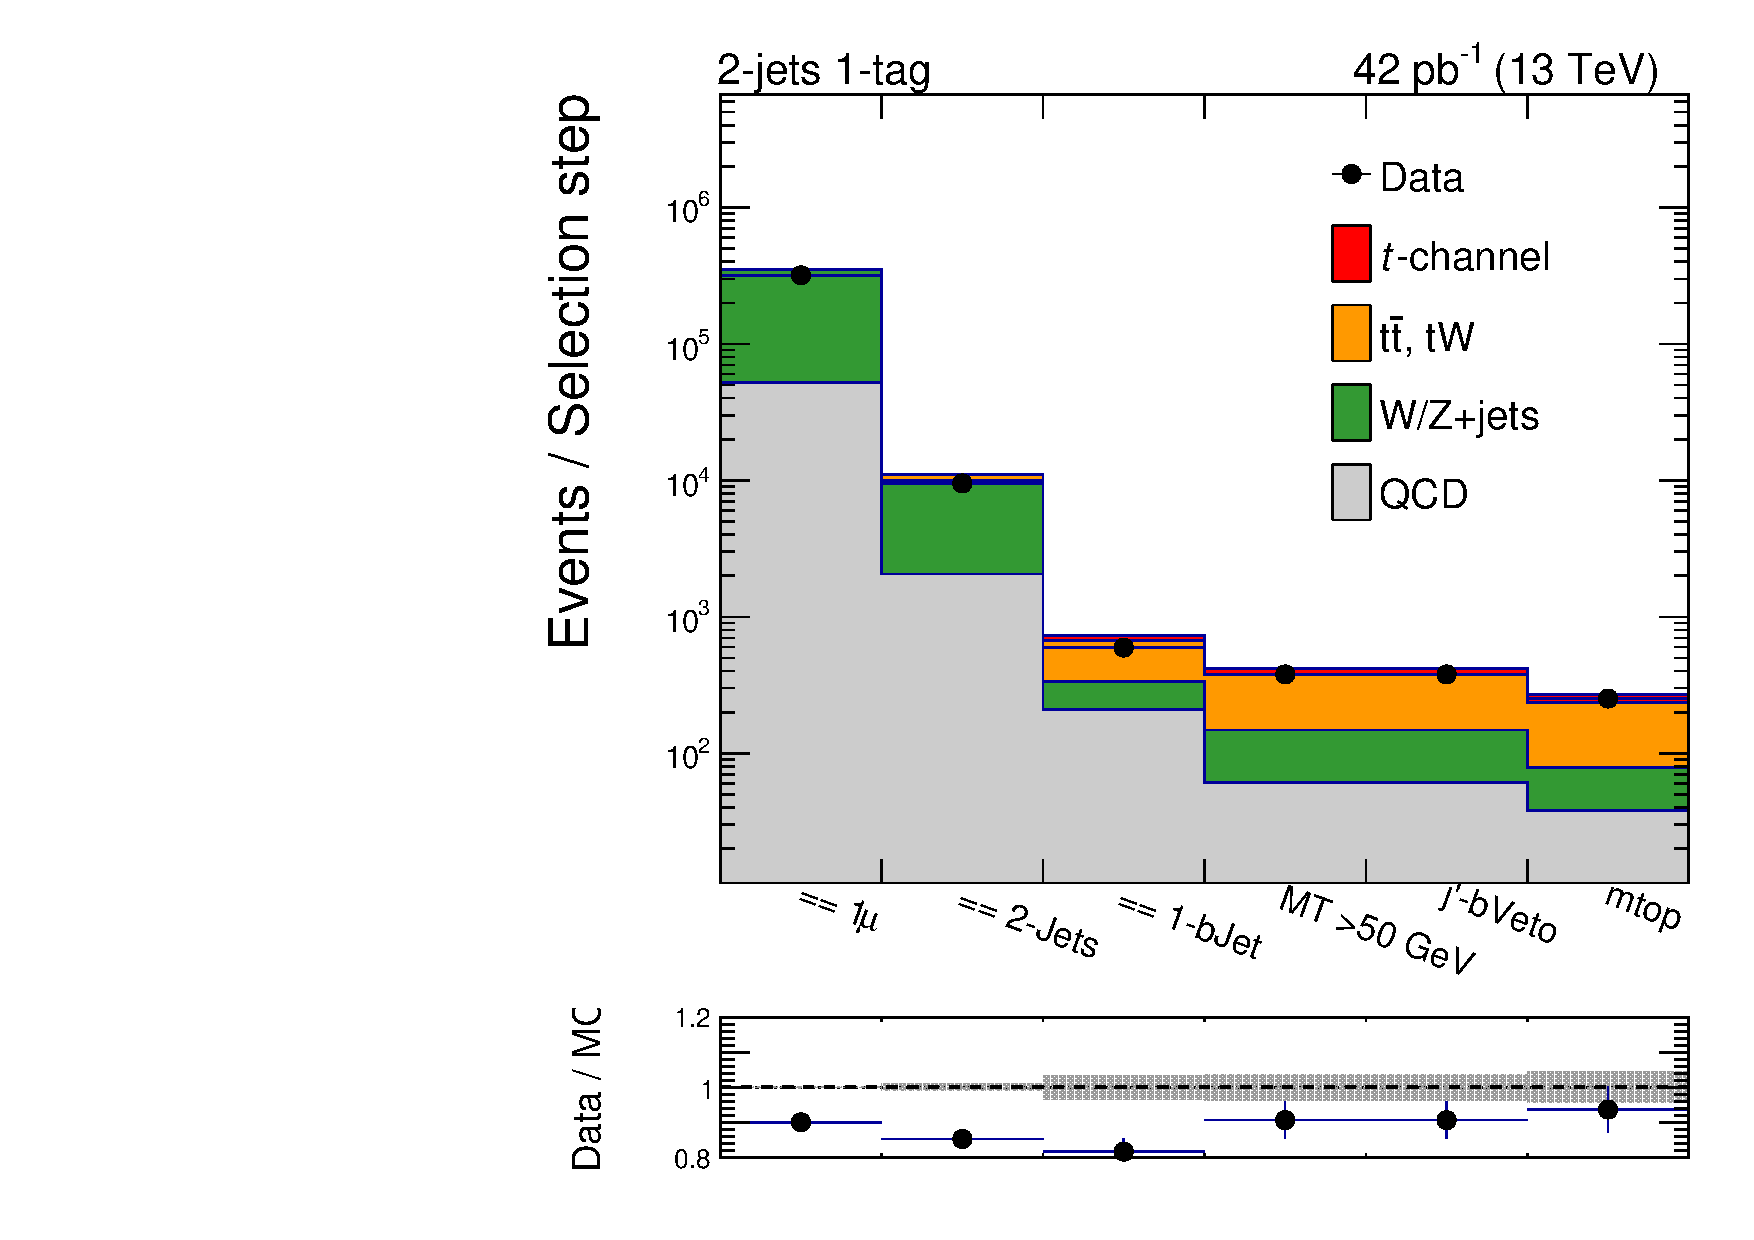
\includegraphics[width=0.6\textwidth]{figures/2J1T/cutflownew.pdf}}
\caption{\label{fig:cutflow}Graphical visualization of the event yields for the different processes after each step of the event selection.}
\end{center}
\end{figure}              
                             
\clearpage

%
%\subsection{Scale factors and reweighting techniques}
%\label{sec:reweighting}
%Scale factors are associated to the selected events in simulation to keep into account further differences between data and MC.
%
%\subsubsection*{Scale factors for b-tagging and mistagging from data}
%\label{sec:btagSF}
%
%Estimates of the selection efficiencies of true and misidentified b-jets 
%can be found in Ref.~\cite{CMS-PAS-BTV-11-004}, as a function of $p_T$ and $\eta$ of the jet.
%Performances are computed for the tight TCHP working point used in this analysis.
%To correct the mistag rates and b-tagging efficiency in simulation each event is weighted by appropriate scale factors, following the procedure explained in Ref.~\cite{rizzi_sf}.
%
%
%\subsubsection*{Pile-up scale factors from data}
%\label{sec:PileUpSF}
%
%One way of evaluating the effect of the PU on the analysis, taking into account the different PU conditions
%during the data taking period, is to determine
%scale factors between the data and simulation. These factors are obtained according 
%to CMS prescriptions: the distribution of the number of true interaction vertices is measured on data, while the 
%same distribution in simulation is known. For each simulated event appropriate weights are applied 
%as a function of the number of interaction vertices, in order to reproduce the distribution of 
%the number of interaction vertices in data (details in Ref.~\cite{pileup_rew}).
%%An example of the true vertices distributions in data and MC is given in Figure ~\ref{fig:truePUEvents}(a),(b) respectively,
%%while Fig.~\ref{fig:truePUEvents}(c),(d) show respectively the the reweighting function obtained from the two and the final 
%%reweighted true distribution function. 
%%
%%It has to be noted that the distribution of weights in Fig.~\ref{fig:truePUEvents}(c) depends on the simulated sample and from the 
%%selection applied, but its average for each sample/selection  is order of 1 with variations of few percents($20\%$ max.).
%%However by construction the weights for events with different pile up multiplicities can differ by as much as 1 or even 2 orders of magnitude.
%%
%%	\begin{figure}[h]
%%	  \begin{center}
%%	    \subfigure[]{
%%	    \includegraphics[width=0.48\textwidth]{figures/selection/PileUpData.png}}
%%	    \subfigure[]{
%%	    \includegraphics[width=0.48\textwidth]{figures/selection/pileUpMC.png}}
%%            \vskip 0.5cm
%%	    \subfigure[]{
%%	    \includegraphics[width=0.48\textwidth]{figures/selection/PileUpWeights.png}}
%%	    \subfigure[]{
%%	    \includegraphics[width=0.48\textwidth]{figures/selection/pileUpRescale.png}}
%%	    \caption{\label{fig:truePUEvents}{True pile up event distribution for data (a), MC(b), rescale function (c) and MC rescaled to data(d).}}
%%	  \end{center}
%%	\end{figure}
%%
%%This can result in the distortion of the shapes of distributions due to the presence of spikes. This effect is more prominent in samples with 
%%low statistics, as shown in figure Fig.~\ref{fig:badcaseexample} and it has potential to be dangerous for samples with higher statistics as well,
%%since it depends on the content of each bin and it is very difficult to keep under control. 
%%
%%The sensitivity of the main variables of this analysis to the pile up, in particular for jets in high pseudorapidity regions, 
%%is first of all studied in the control samples, as it is shown in Sec.~\ref{sec:wjets}. The cuts $p_T>60$~GeV for the two leading jets and $RMS < 0.025$ for the untagged jets are introduced to reduce this sensitivity 
%%and keep the shapes of the variables under control as a baseline strategy.
%%
%%Our strategy for mitigating the effect of the pile up is discussed in the following chapters, in particular Sec.~\ref{sec:wjets}. 
%%%%FIXME:whenever we add it,we uncomment it 
%%%%Section~\ref{sec:pileUp} is dedicated to our strategy for mitigating the pileup effects. 
%%
%%	\begin{figure}[h]
%%	  \begin{center}
%%	    \subfigure[]{
%%	    \includegraphics[width=0.48\textwidth]{figures/selection/3J_1TleptonPtWithPUMuStack.png}}
%%	    \subfigure[]{
%%	    \includegraphics[width=0.48\textwidth]{figures/selection/3J_1TleptonPtNoPUAfterCutsSR_PUWPMuStack.png}}
%%	    \caption{\label{fig:badcaseexample}{Example of reweighted distribution where the spikes due to pile up reweighting alter the shape in
%%	    an unphysical way: muon \pt in the sample where 3 jets ($p_T > 40$~GeV, no $RMS$ cut) are required, one of which b-tagged with (a) and without (b) pile up reweighting, normalized to data yield.}}
%%	    \end{center}
%%	\end{figure}
%%
%%
%%
%%This can be understood looking at the distribution of number of vertices of data and simulation: looking at figure ~\ref{fig:PUs} one can qualitatively expect that 
%%events in regions where data-MC distributions of number of vertices don't overlap will have a low weight and vice versa for events in overlapping regions.
%% Figure~\ref{fig:PUFuncs} confirms this, showing that most of the events in the MC samples have small weights due to the fact that they are in non-overlapping
%%regions in number of vertices. 
%%Those figures refer to two different MC distributions, the one in Figg.~\ref{fig:PUs}(b),~\ref{fig:PUFuncs}(b) having an overall better match with data.
%%
%%Therefore a solution we adopt is to use an overall scale factor for samples with a distribution like those in Figg.~\ref{fig:PUs}(a),~\ref{fig:PUFuncs}(a), 
%%and an event-by-event scale factor for samples with a distribution like those in Figg.~\ref{fig:PUs}(b),~\ref{fig:PUFuncs}(b). 
%%
%%The former is taken sample by sample as the average of the pile up weights of all events composing that sample, and it is always very close to 1 as expected.
%%
%%	\begin{figure}[h]
%%	  \begin{center}
%%	    \subfigure[]{
%%	    \includegraphics[width=0.48\textwidth]{figures/selection/DataVsSummer12PU.png}}
%%	    \subfigure[]{
%%	    \includegraphics[width=0.48\textwidth]{figures/selection/DataVsSummer12V6PU.png}}
%%	    \caption{\label{fig:PUs}{MC (red continuous line) vs data (blue dots) distributions of number of true pile up interactions. 
%%The MC distribution in (a) refers to the ``PU-S7'' production, while (b) refers to the ``PU-S6'' distribution, both described in ~\cite{PUPVTPage}.}}
%%	    \end{center}
%%	\end{figure}
%%
%%
%%	\begin{figure}[h]
%%	  \begin{center}
%%	    \subfigure[]{
%%	    \includegraphics[width=0.48\textwidth]{figures/selection/PUWeight_vs_nVertices.png}}
%%	    \subfigure[]{
%%	    \includegraphics[width=0.48\textwidth]{figures/selection/PUWeight_vs_nVertices_TTBar.png}}
%%	    \caption{\label{fig:PUFuncs}{2D plot of pile up weight vs number of true pile up interactions, mapping Monte Carlo distribution
%%	    to data distributions shown in Fig. ~\ref{fig:PUs}. }}
%%	    \end{center}
%%	\end{figure}
%

%\clearpage

\section{Trigger and muon efficiencies}
\label{sec:muonEff}
\subsection{Muon identification and isolation efficiencies}
\label{sec:muonEff1}
Muon efficiencies are measured with the tag and probe method using
$Z\rightarrow\mu^{+}\mu^{-}$ events. Identification and isolation efficiencies are estimated for exactly the same selection used in the analysis with the standard tag and probe package in CMSSW. A fit is performed on the ($\mu^{+}\mu^{-}$) invariant mass distribution in order to determine the number of signal and background events in the mass peak. 
The results from data are compared to
efficiencies measured in Drell-Yan MC (with pileup corrections applied), and data-to-MC
scale factors are derived ($SF = \varepsilon^{data}/\varepsilon^{MC}$) used to correct the MC
predictions. Single muon triggered data sample is used as listed in Table~\ref{tab:samples}.


\begin{table}
\vspace{0.2cm}
\begin{center}
\begin{tabular}{l|l}
\hline
Data Sample & Dataset \\
\hline
\hline
SingleMuon     & /SingleMuon/Run2015B-PromptReco-v1/AOD \\
\hline
\end{tabular}
\caption{Data sample used for muon efficiency measurements. The integrated luminosity used for the results in this section corresponds to 40~pb$^{-1}$.}
\label{tab:samples}
\end{center}
\end{table}

%The lepton identification and isolation efficiencies are estimated sequentially. %The identification efficiency corresponds to the number of probe leptons passing the complete selection criteria except from the isolation requirement over the total number of probe leptons. The isolation efficiency is defined as the ratio between leptons passing the selection criteria and the isolation cut and the total number of leptons passing the previous identification requirements. 

%Dilepton candidates compatible with the Z mass are assumed to come from the Z bosons and used to estimate the efficiency. 
%The tag and probe leptons are matched requiring opposite charge and an invariant mass in the range 60 $<$ m$_{ll}$ $<$ 120 GeV. 
The muon identification and isolation efficiencies are measured sequentially. Opposite charge dimuon candidates with an invariant mass in the range 70 $<$ m$(\mu^{+}\mu^{-})$ $<$ 130 GeV are used in the measurement. The definition of tag leptons is chosen tight enough to provide a clean signal sample. Tag muons are required to pass the Tight muon ID definition and to have $\pt$ larger than 25 $\GeV$, $|\eta| < 2.1$ and relative PF isolation of less than 0.2 with $\Delta\beta$ corrections applied. In addition, tags are required to be associated to an HLT lepton for trigger bit HLT\_IsoMu20, which is unprescaled for the considered data taking period. General tracks (tight ID muons) are used as probes for the muon ID (isolation) efficiencies. The passing probe muons, for which the efficiency is measured, pass the same ID and isolation selection as used in the analysis. 
%The definition of "tag" electrons corresponds to the complete electron selection, isolation and identification used in the analysis. In the case of muons, tag leptons are required to pass a tighter criteria than the one used in the analysis, to have a cleaner sample. This criteria involves requirements in the transverse impact parameter, number of hits in the muon chambers and tracker detectors and quality of the track fit. 
The signal component in the resulting
($\mu^{+}\mu^{-}$) invariant mass distribution is fit with a sum of
two Voigtians, the background component is fit with exponential. The muon identification and isolation efficiencies and scale factors are presented in 
Figures~\ref{fig:muonEff_ID} and ~\ref{fig:muonEff_Iso}. 
%Table~\ref{tab:muoneff} (muons) and Table~\ref{tab:eleceff} (electrons) present the total efficiencies and scale factors. XXX FIXME

\begin{figure}[htbp!]
  \begin{center}
    \resizebox{0.48 \textwidth}{!}{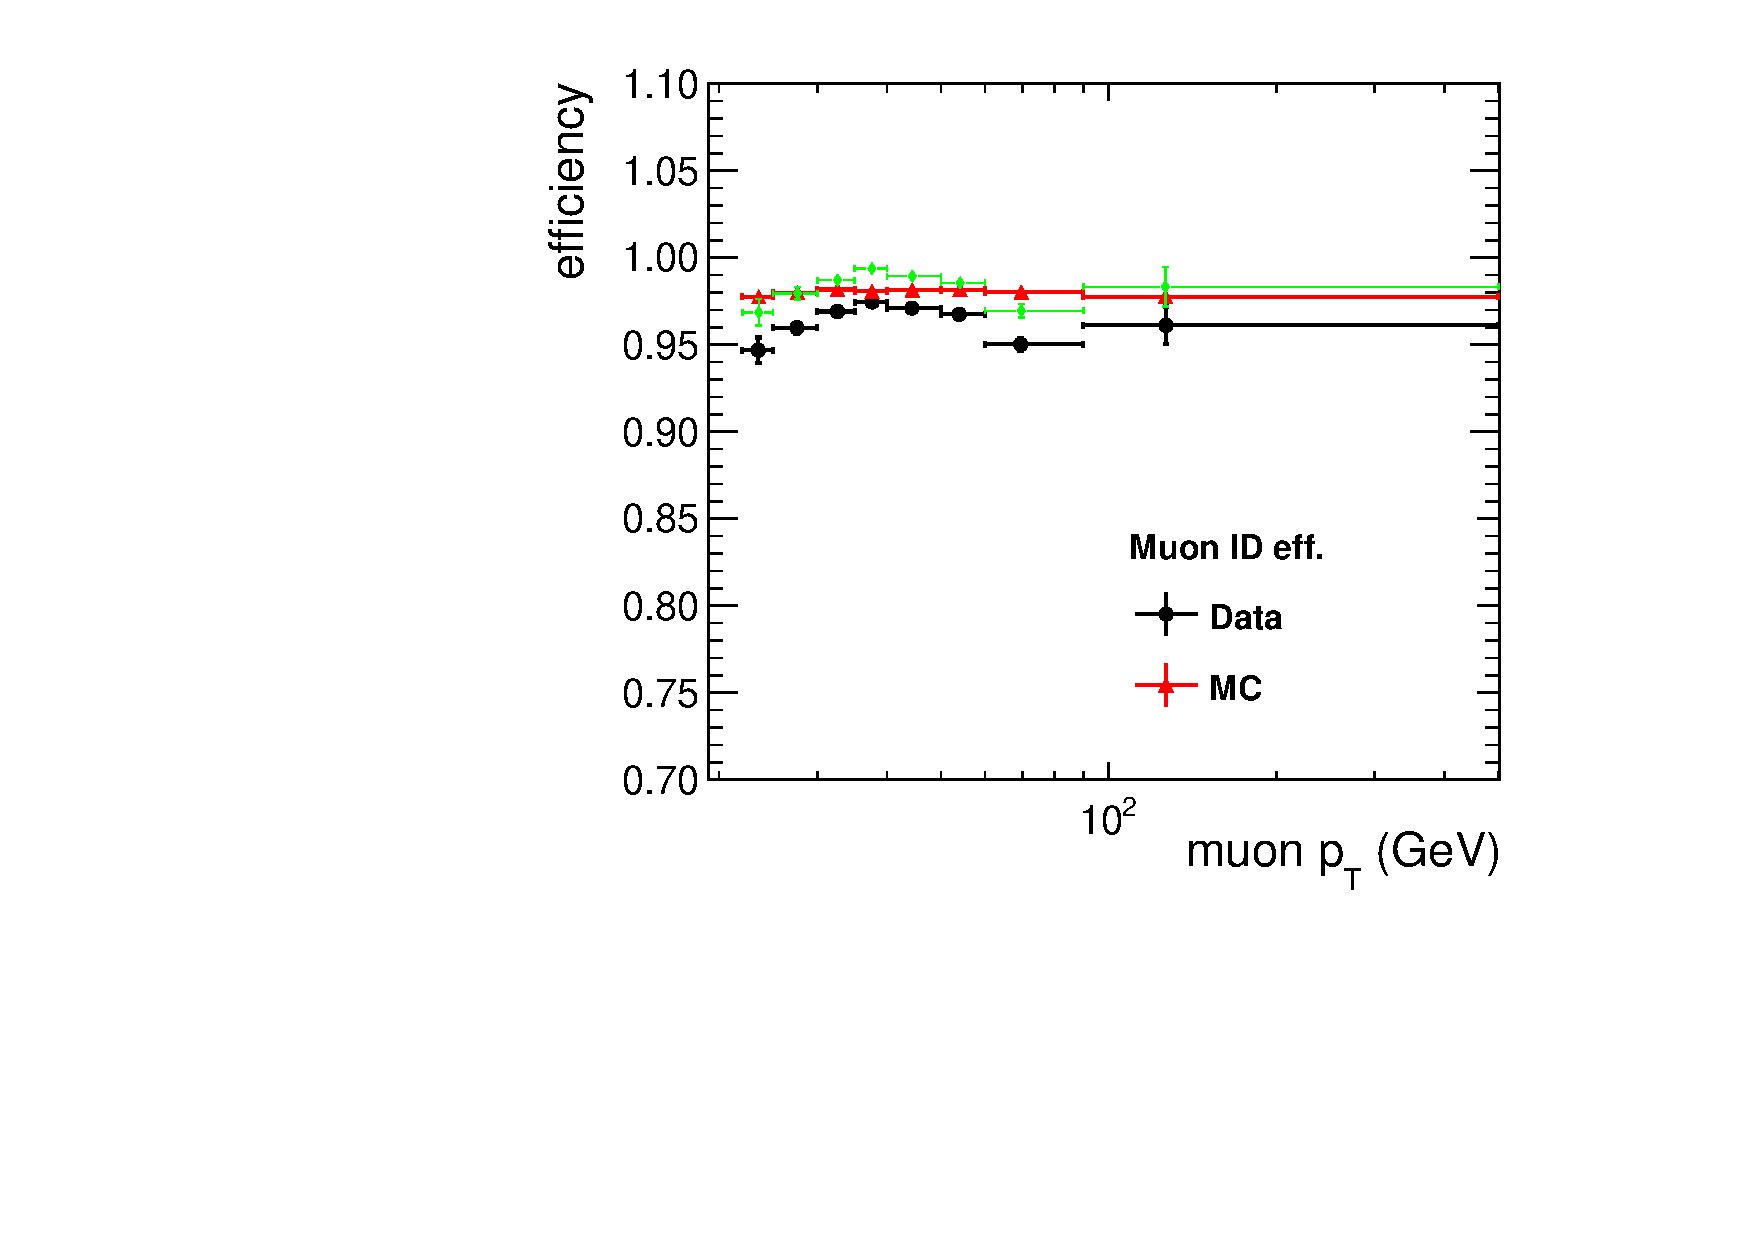
\includegraphics{figures/Figures_MuonEff/muon_ID_pt}}
    \resizebox{0.48 \textwidth}{!}{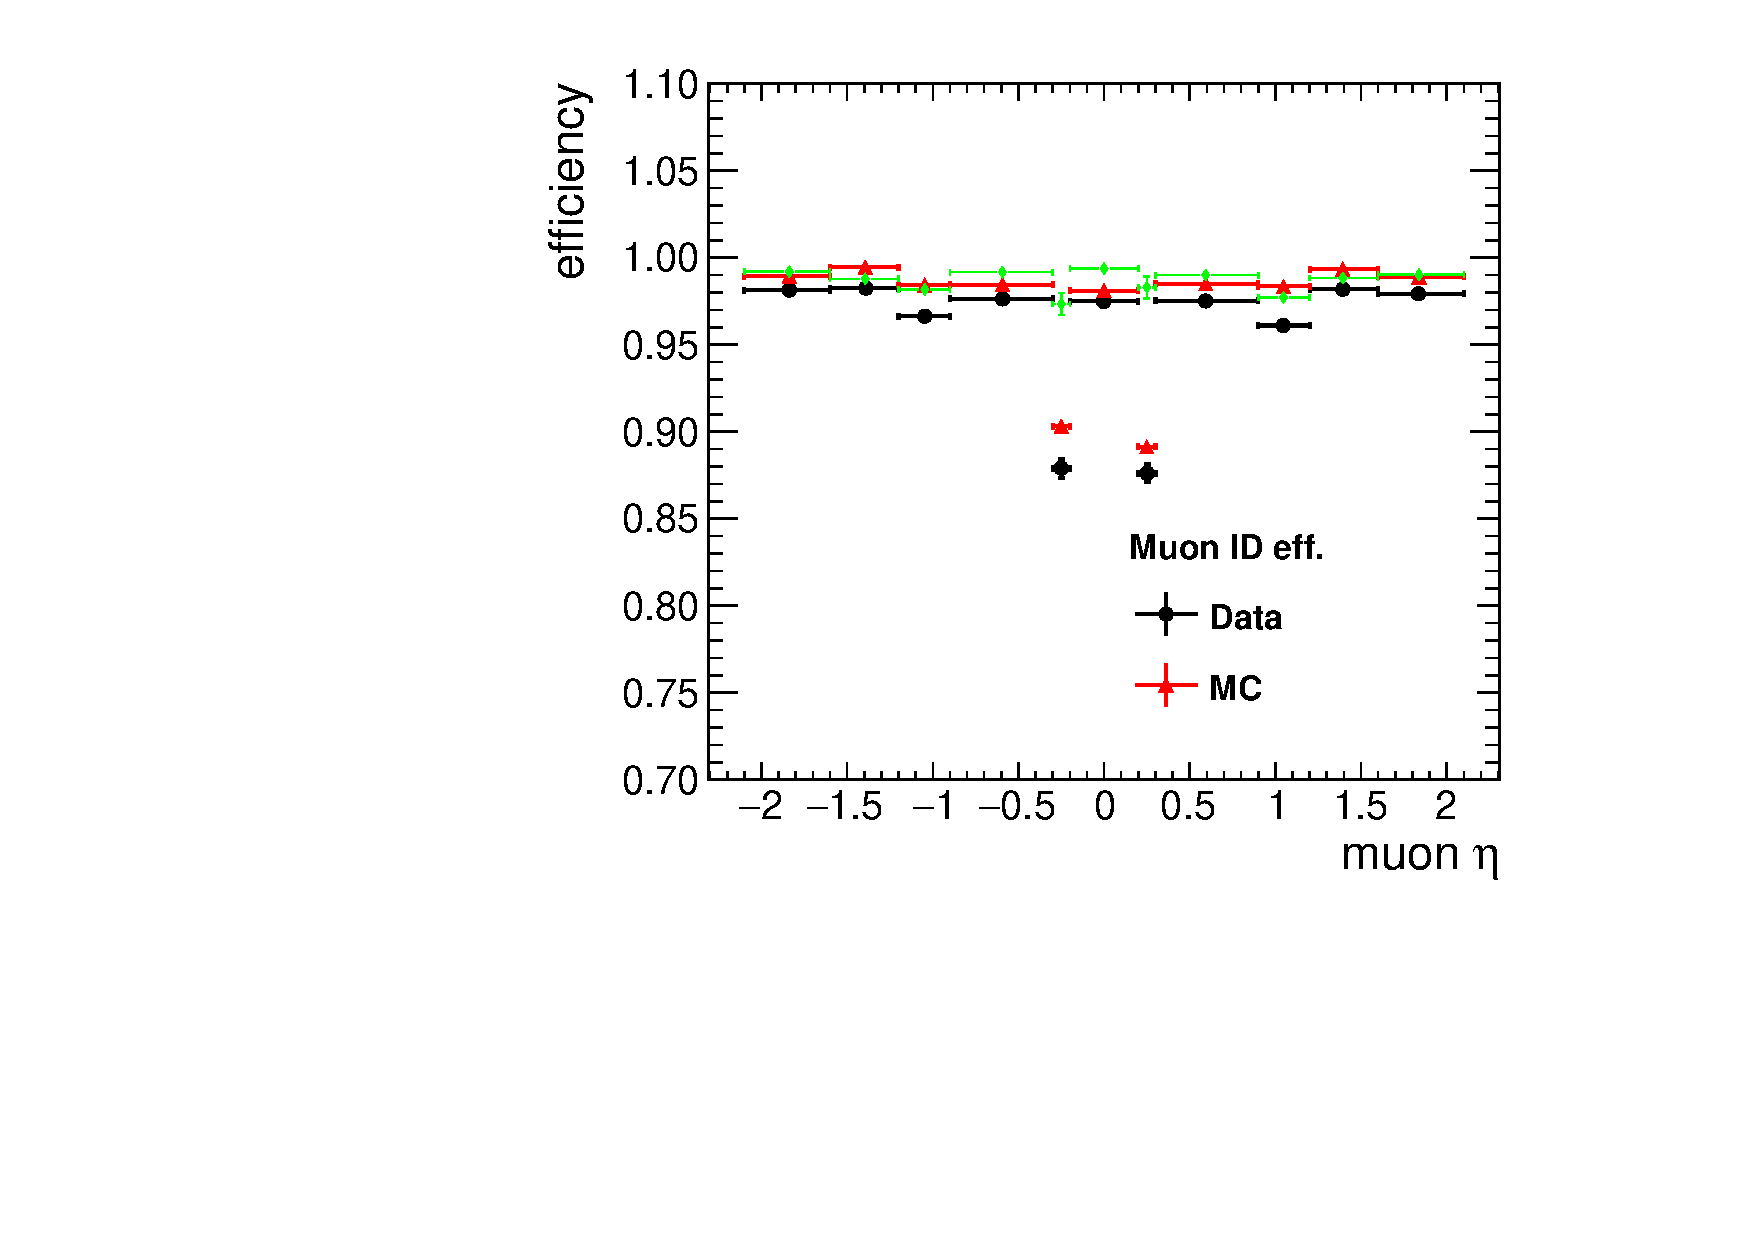
\includegraphics{figures/Figures_MuonEff/muon_ID_eta}}
      \caption{Muon identification efficiency (tight muon definition) in data (black), MC (red) and data-to-MC
        scale factors (green) as a function of muon \pt (left) and $\eta$ (right). Uncertainties are statistical only.}
\label{fig:muonEff_ID}
  \end{center}
\end{figure}


\begin{figure}[htbp!]
  \begin{center}
    \resizebox{0.48 \textwidth}{!}{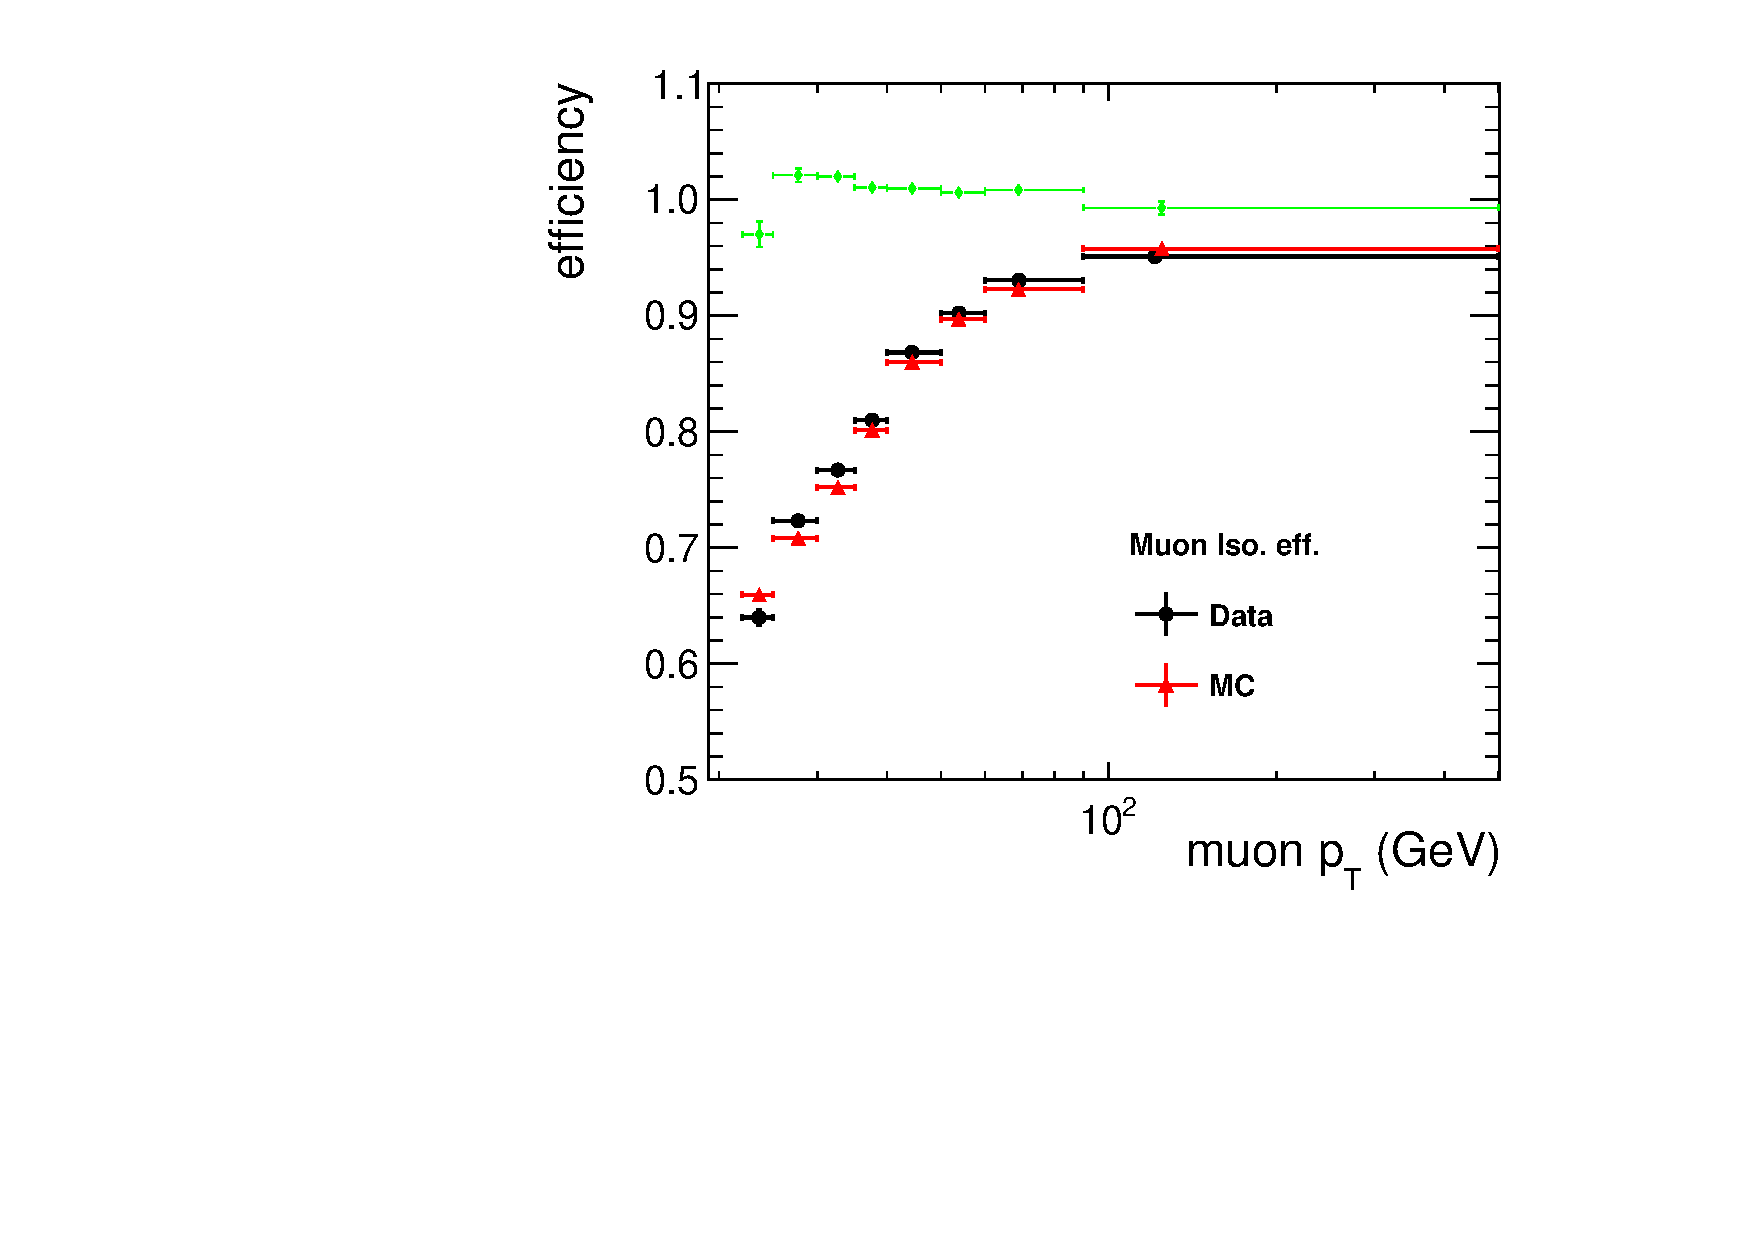
\includegraphics{figures/Figures_MuonEff/muon_Iso_pt}}
    \resizebox{0.48 \textwidth}{!}{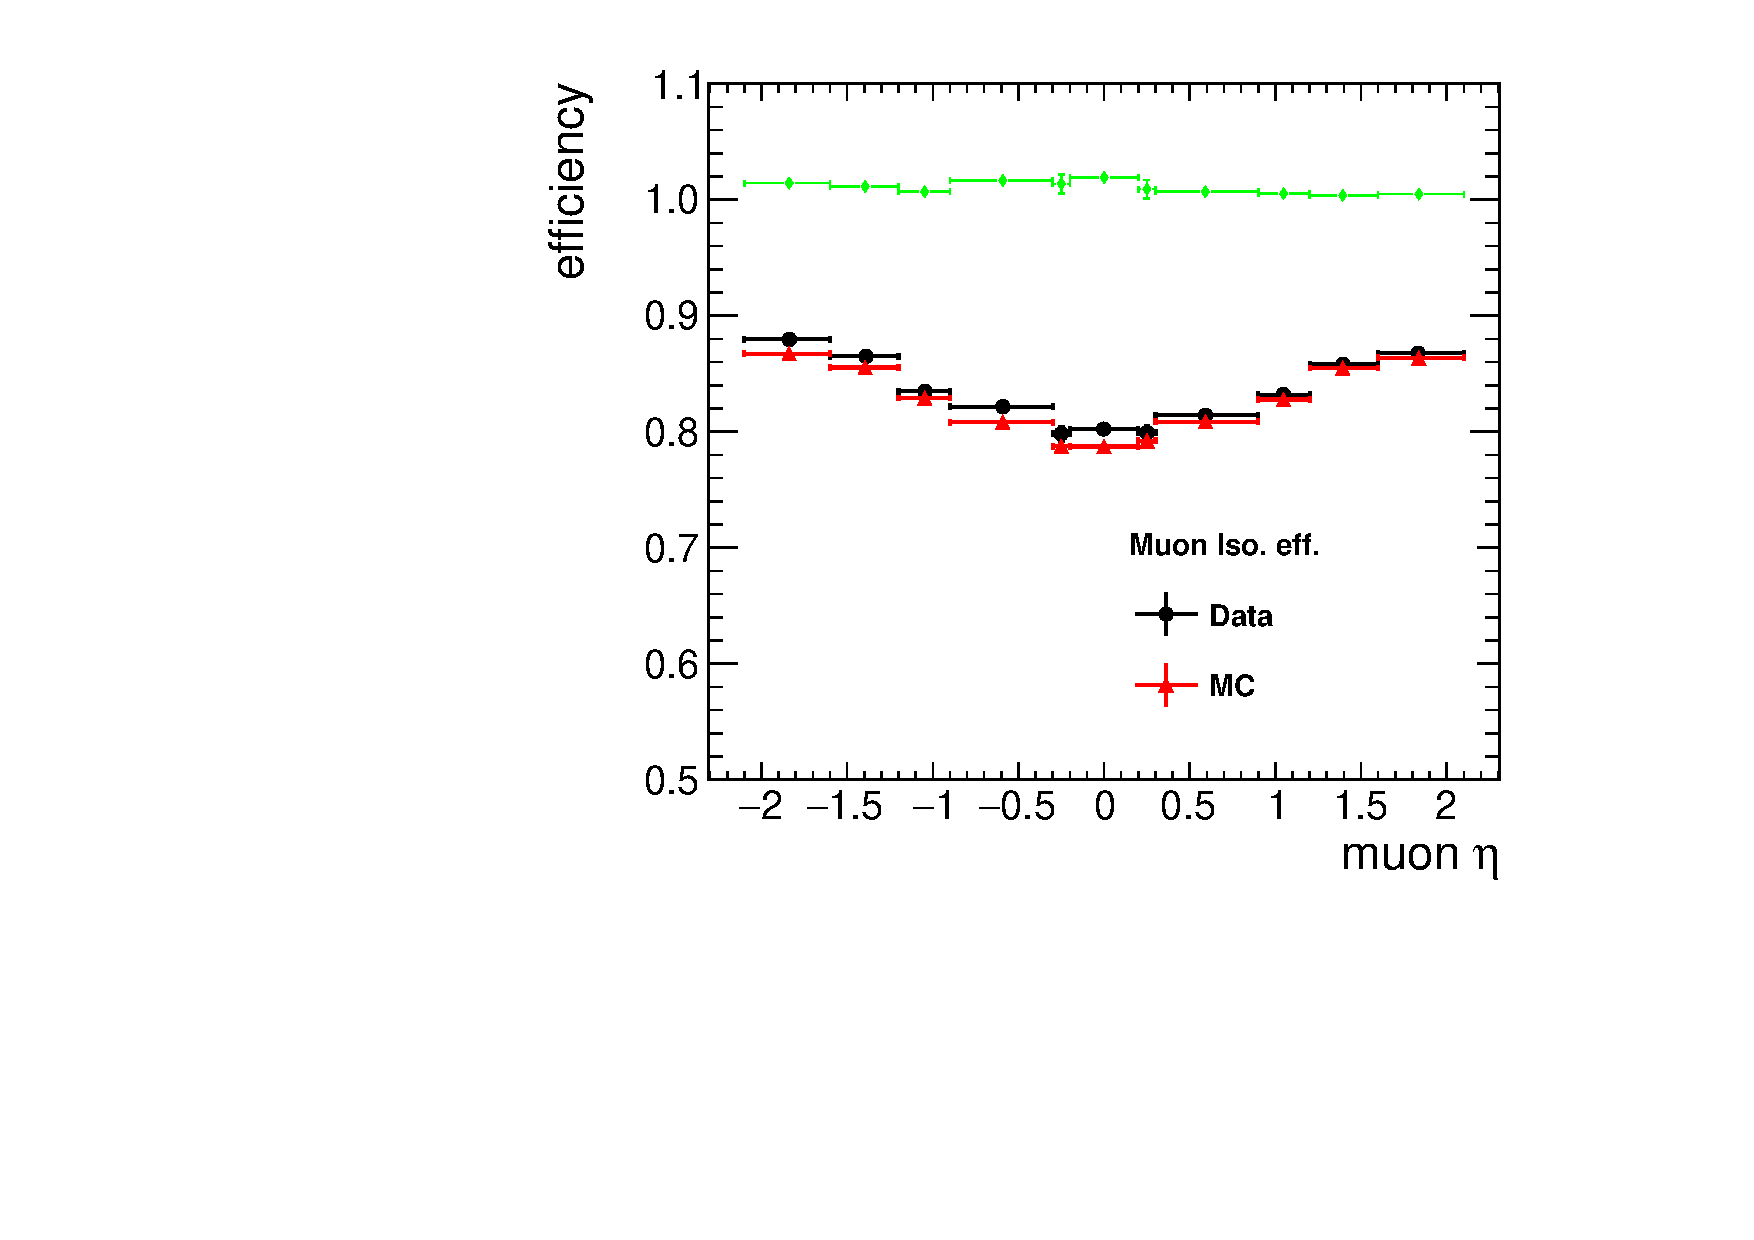
\includegraphics{figures/Figures_MuonEff/muon_Iso_eta}}
      \caption{Muon isolation efficiency in data (black), MC (red) and data-to-MC
        scale factors (green) as a function of muon $\pt$ (left) and $\eta$ (right). Uncertainties are statistical only.}
\label{fig:muonEff_Iso}
  \end{center}
\end{figure}


Systematic uncertainties are estimated by varying the tag muon selection, the signal and background pdfs and the invariant mass window for the fit, and reapplying the tag and probe method. The largest variation of the scale factors with respect to their nominal values is taken as uncertainty of the scale factors. Additional uncertainty is also considered accounting  for the different topology of leptons coming from top decays and Z boson decays. A systematic uncertainty of 1$\%$ is applied on the muon ID scale factors, and between 1.5$\%$ and 2.5$\%$ (depending on the bin) on the isolation scale factors.
%To take into account the different topology of leptons coming from the top decay and Z decays, a more conservative systematic uncertainty of 2\% (preliminary) is used for the global values. 
Figure~\ref{fig:topSFmu1} shows the scale factors as a function of $(|\eta|,p_T)$ of the muon, which are used to correct the MC predictions in the analysis.

\begin{figure}[htbp!]
  \begin{center}
      \resizebox{ \textwidth}{!}{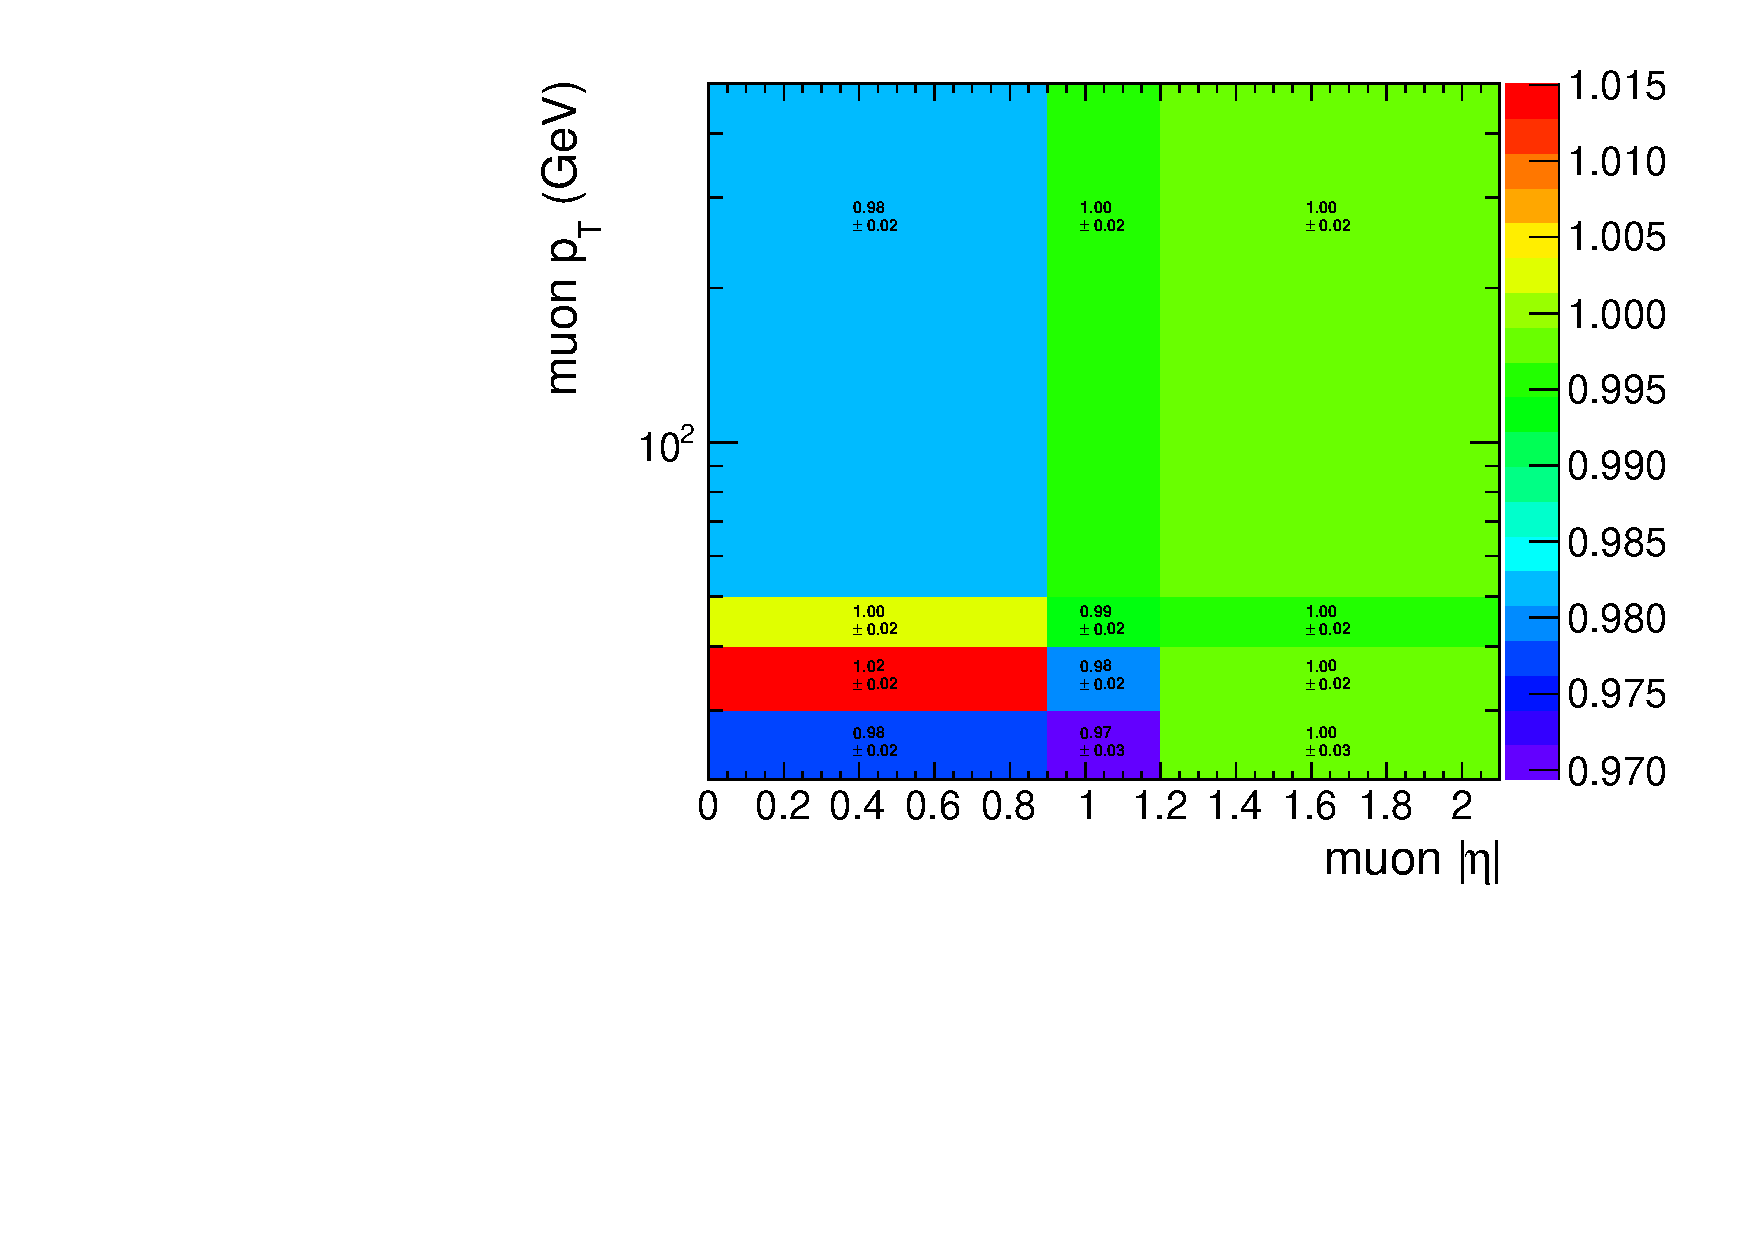
\includegraphics[width=1.1\textwidth]{figures/Figures_MuonEff/muon_IDxIso_2d.pdf}}%
  \end{center}
   \caption{Scale factors accounting for Identification x Isolation efficiencies as a function of ($|\eta|$, p$_T$) of muons. The uncertainties in the plot correspond to the  statistical and systematic uncertainties added in quadrature. The scale factors are in the range 0.97-1.02 and the total uncertainties are of the order of 2-3$\%$ in the different bins.}
  \label{fig:topSFmu1}
\end{figure}






%%%%%%%%%%%%%%%%%%%%%%%%%%%%%%%%%
\subsection{High level trigger efficiency}
\label{subsec:hlt}
To maximize the trigger efficiency, the trigger bit ''HLT\_IsoMu20\_eta2p1'' is combined through a logical ''OR'' with the bit ''HLT\_IsoTkMu20\_eta2p1'' which uses a tracker muon HLT algorithm. 
The efficiency of ''HLT\_IsoMu20\_eta2p1 OR HLT\_IsoTkMu20\_eta2p1'' is also measured with the tag and probe method as described in Section \ref{sec:muonEff1}. The same tag muon selection is used as in the ID and isolation efficiency measurement. The probe muons pass the full lepton selection  used in the analysis, the passing probe muons in addition are matched to the trigger bit of interest. The measured single muon efficiencies and scale factors are shown in Figure~\ref{fig:muonEff_HLT_IsoMu20}. Figure~\ref{fig:topSFmu2} shows the scale factors as a function of $(|\eta|,p_T)$ of the muon, which are used to correct the MC predictions in the analysis. The estimated systematic uncertainty of the scale factors is of the order of 1-1.5$\%$.

\begin{figure}[htbp!]
  \begin{center}
    \resizebox{0.48 \textwidth}{!}{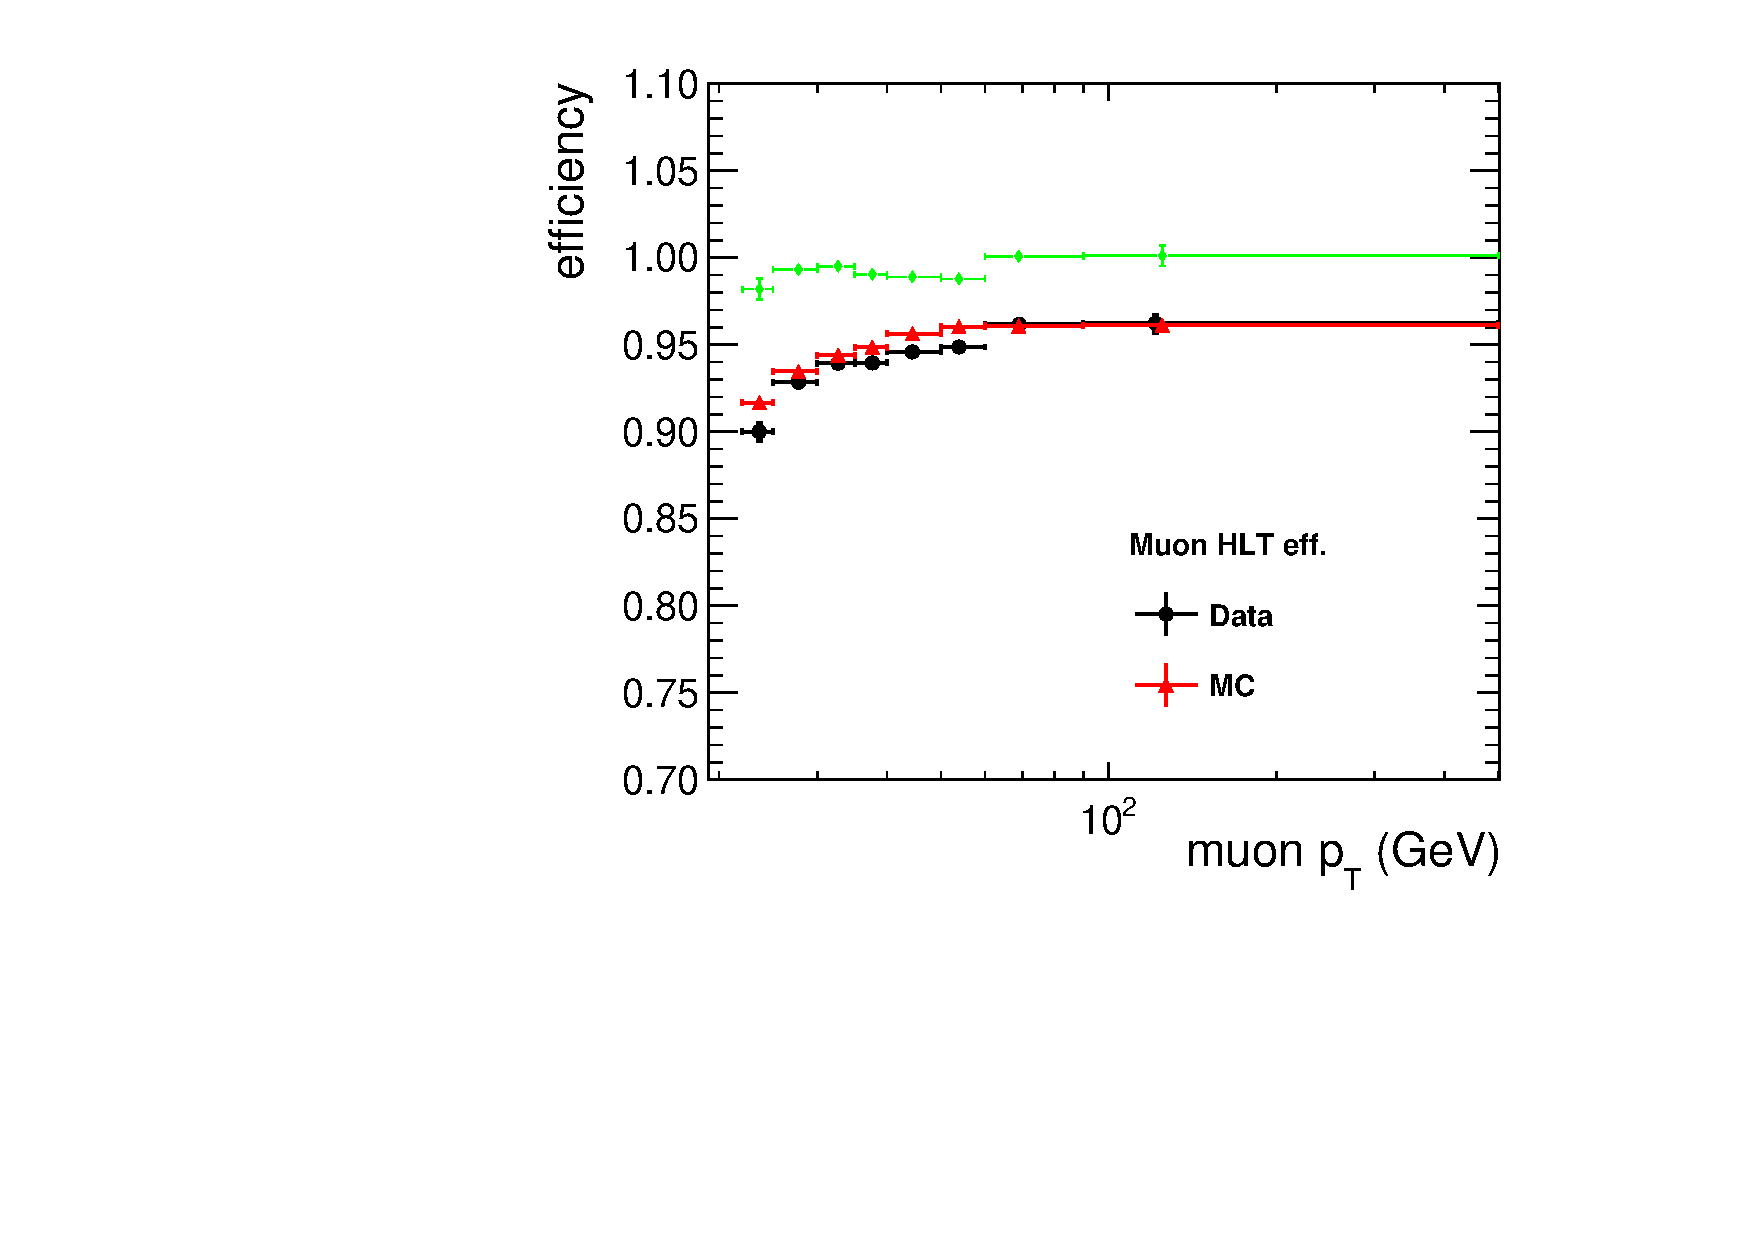
\includegraphics{figures/Figures_MuonEff/muon_HLT_pt}}
    \resizebox{0.48 \textwidth}{!}{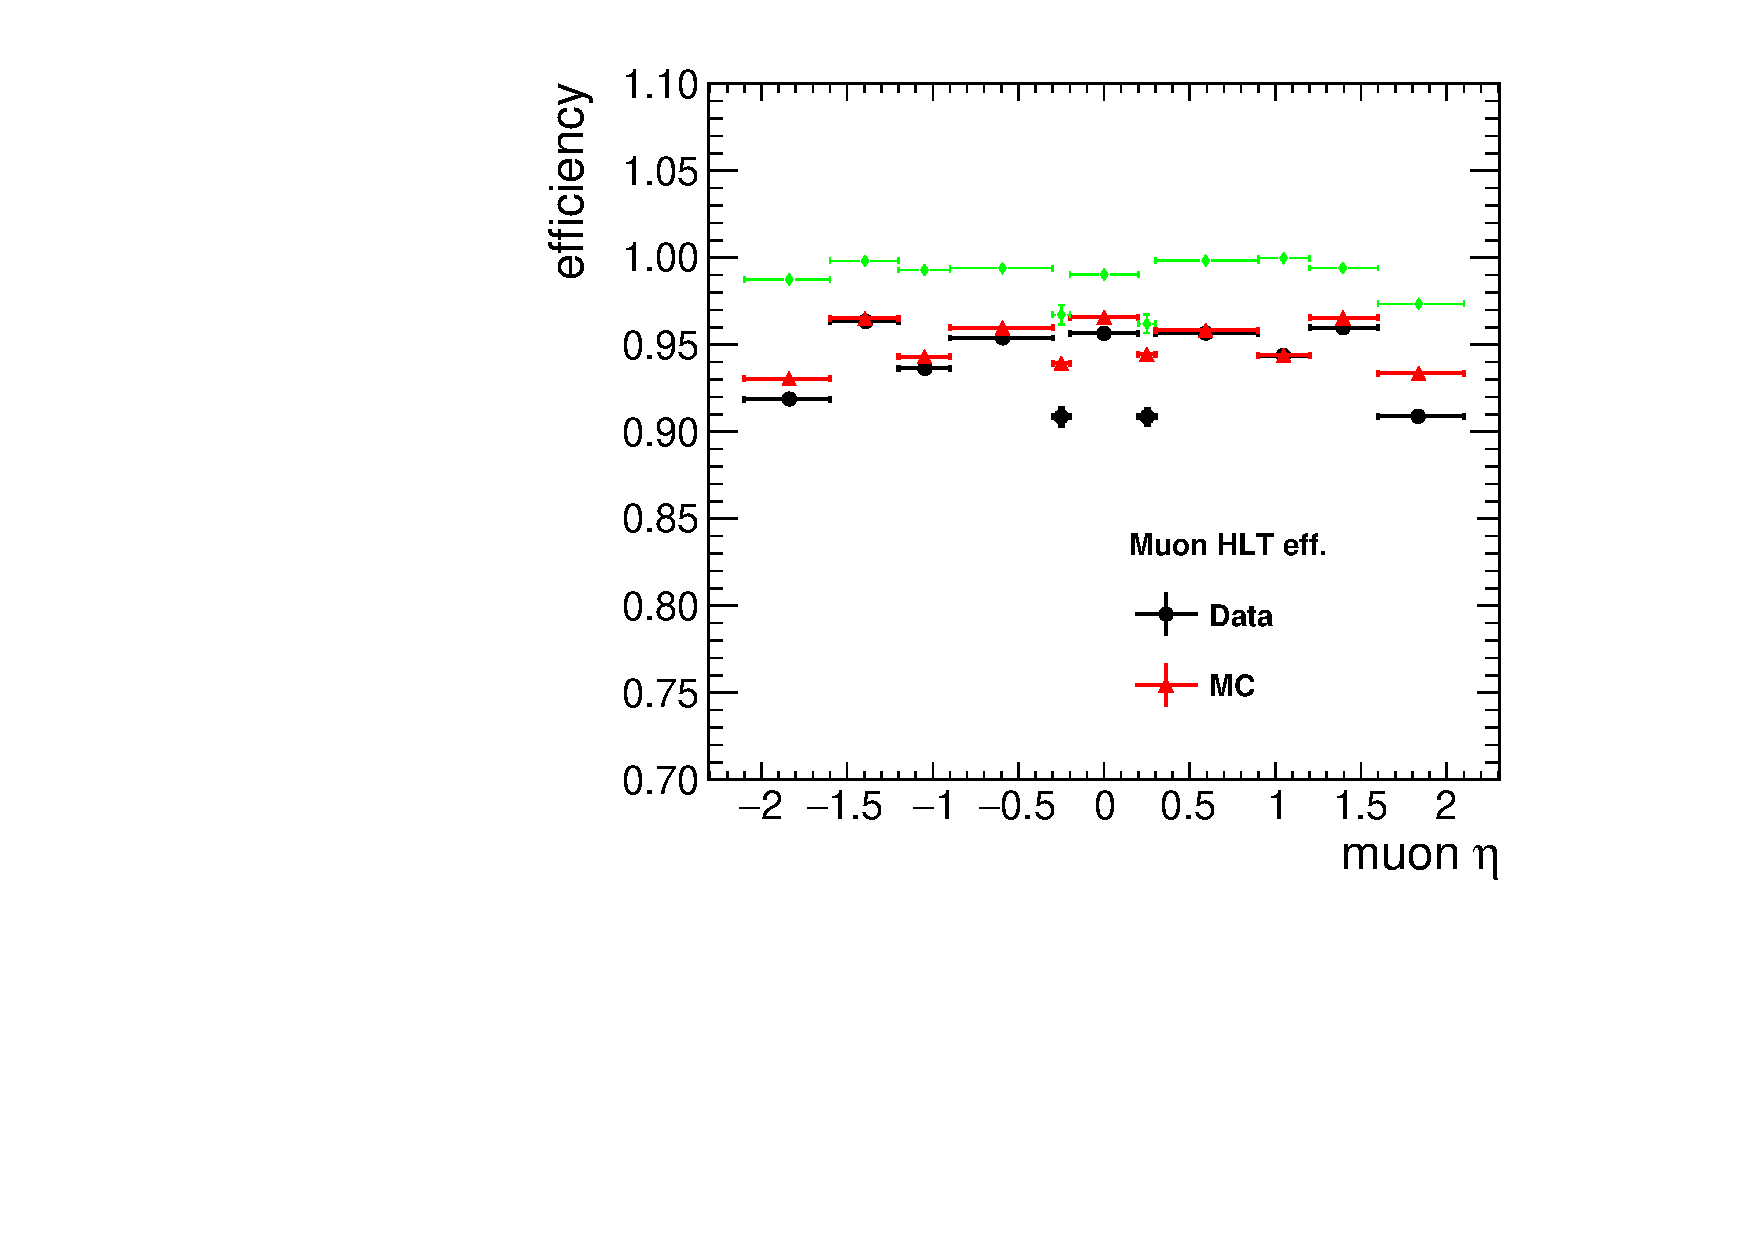
\includegraphics{figures/Figures_MuonEff/muon_HLT_eta}}
      \caption{Efficiency of the single muon triggers ''HLT\_IsoMu20\_eta2p1 OR HLT\_IsoTkMu20\_eta2p1'' for data (black), MC (red) and data-to-MC
        scale factors (green) as a function of muon $\pt$ (left) and $\eta$ (right). Uncertainties are statistical only.}
\label{fig:muonEff_HLT_IsoMu20}
  \end{center}
\end{figure}



\begin{figure}[htbp!]
  \begin{center}
   \resizebox{ \textwidth}{!}{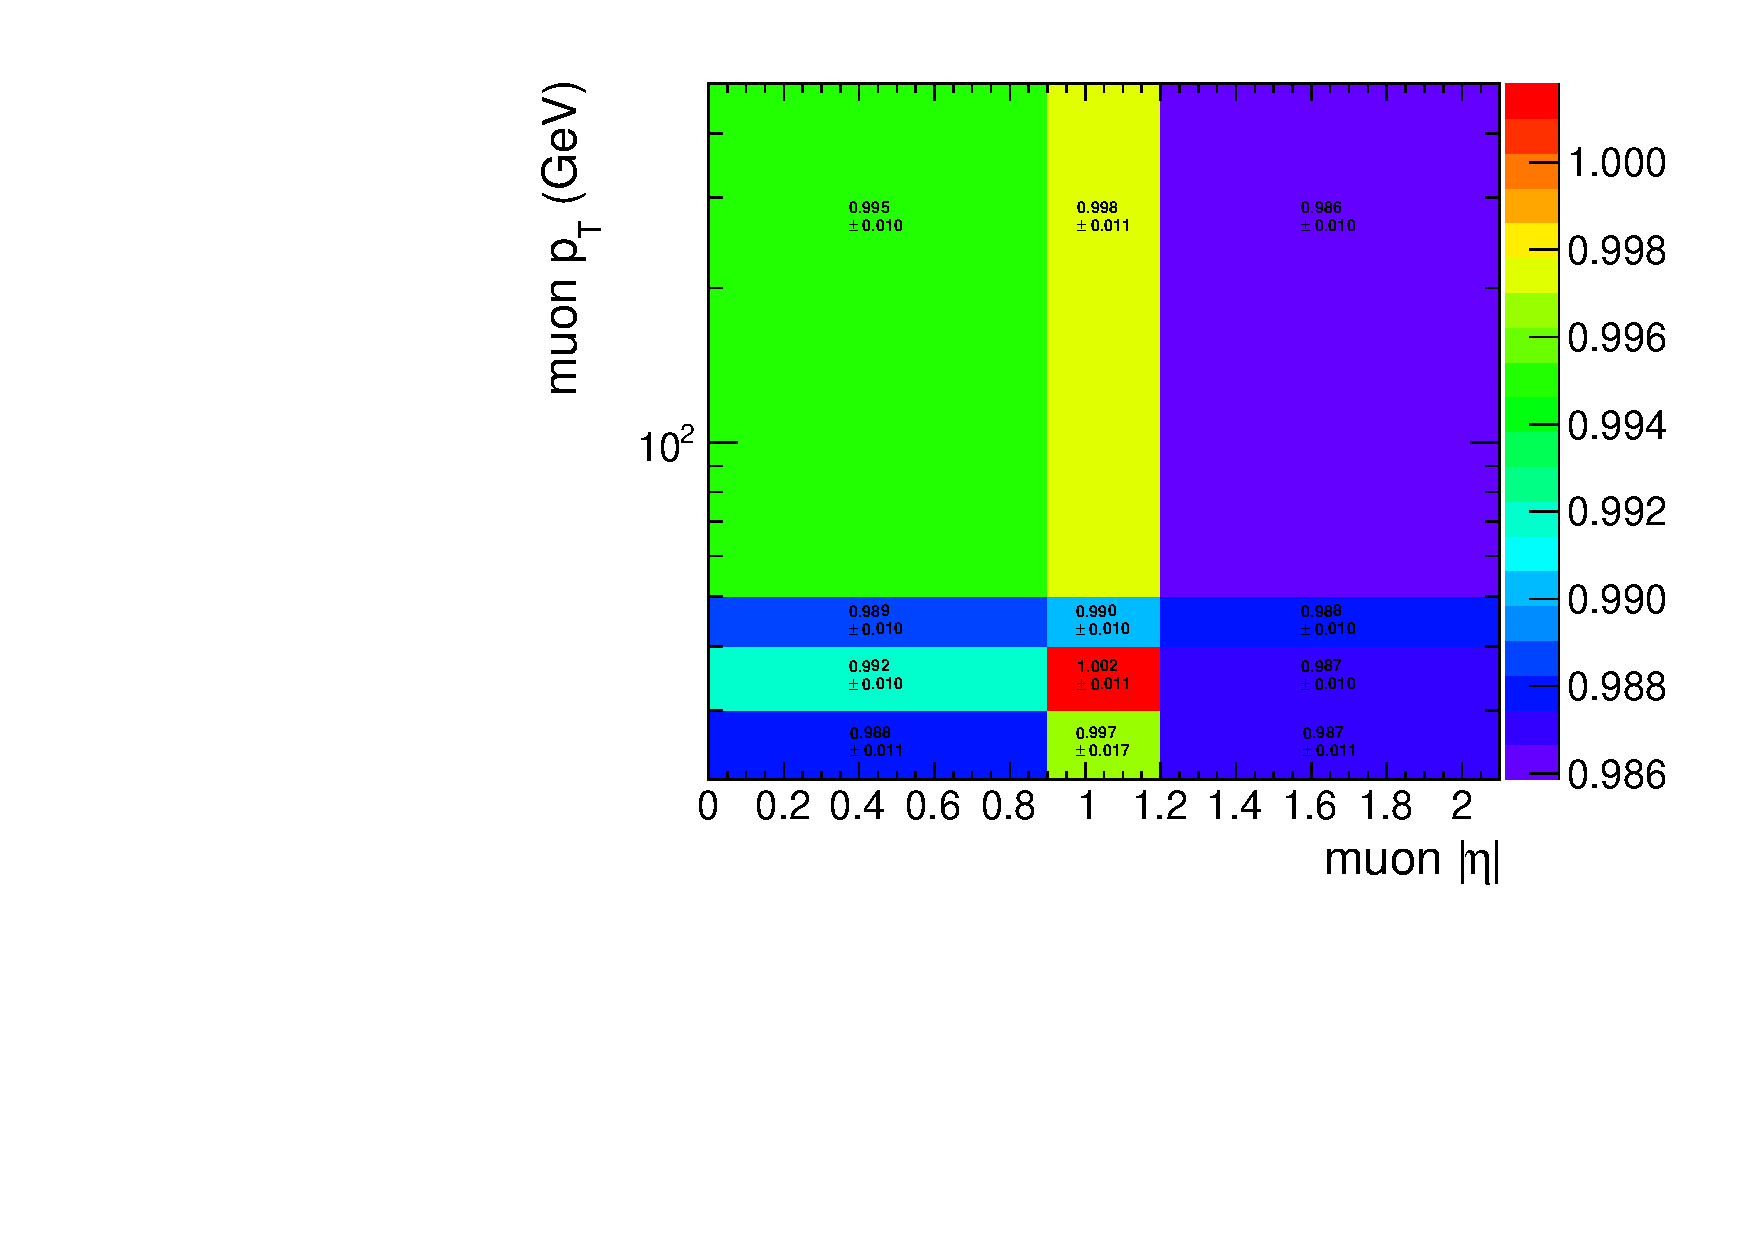
\includegraphics[width=1.2\textwidth]{figures/Figures_MuonEff/muon_HLT_2d}}%
  \end{center}
   \caption{Data-to-MC scale factors accounting for ''HLT\_IsoMu20\_eta2p1 OR HLT\_IsoTkMu20\_eta2p1'' efficiency. The uncertainties in the plot correspond to the  statistical and systematic uncertainties added in quadrature. The scale factors are in the range 0.98-1.00 and the uncertainties are of the order of 1-2$\%$.}
  \label{fig:topSFmu2}
\end{figure}



\clearpage


\section{Control plots}
\label{sec:controlplots}
\subsection{2J0T Control region}

The 2J0T control region is dominated by $W$+light flavor jets (and \QCD) events. In order to test the modelling of this background component, the distributions of several kinematic variables are studied. The distributions of the relevant background processes are normalized to their MC-predicted yields, summed up, and compared to the distributions from data.  Figure~\ref{fig:Jets2J0T} shows the p$_{T}$ and absolute value of $\eta$ distributions of the "light" jet (here: the more forward jet) and the "b-tagged" jet (here: the more central jet). Figure~\ref{fig:Mu_MET_2J0T} shows the distribution of the transverse momentum and the rapidity of the muon, the missing transverse energy of the event and the transverse mass of the neutrino-muon system.



\begin{figure}[hbpt]
\begin{center}
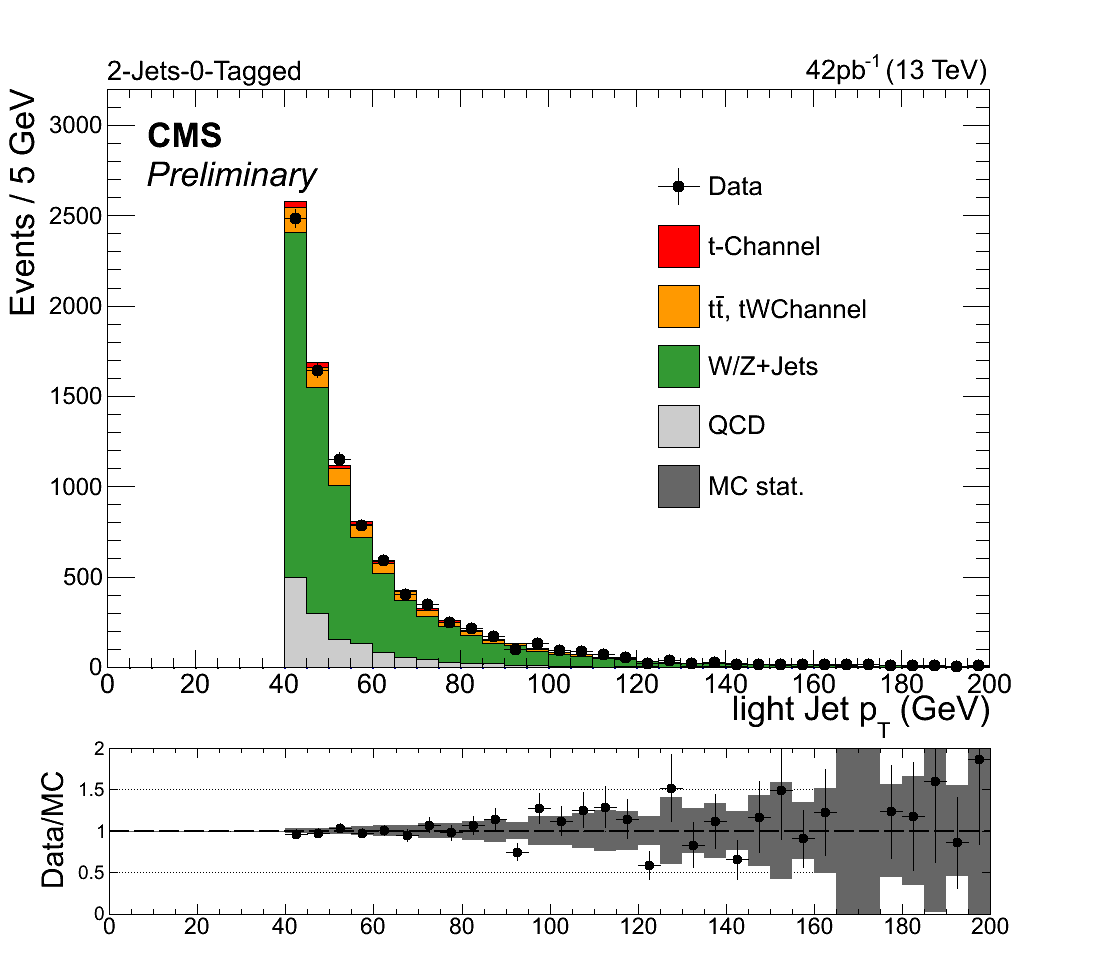
\includegraphics[width=0.45\textwidth,height=0.4\textwidth]{figures/2J0T/Sep8/lightJetPt.png}
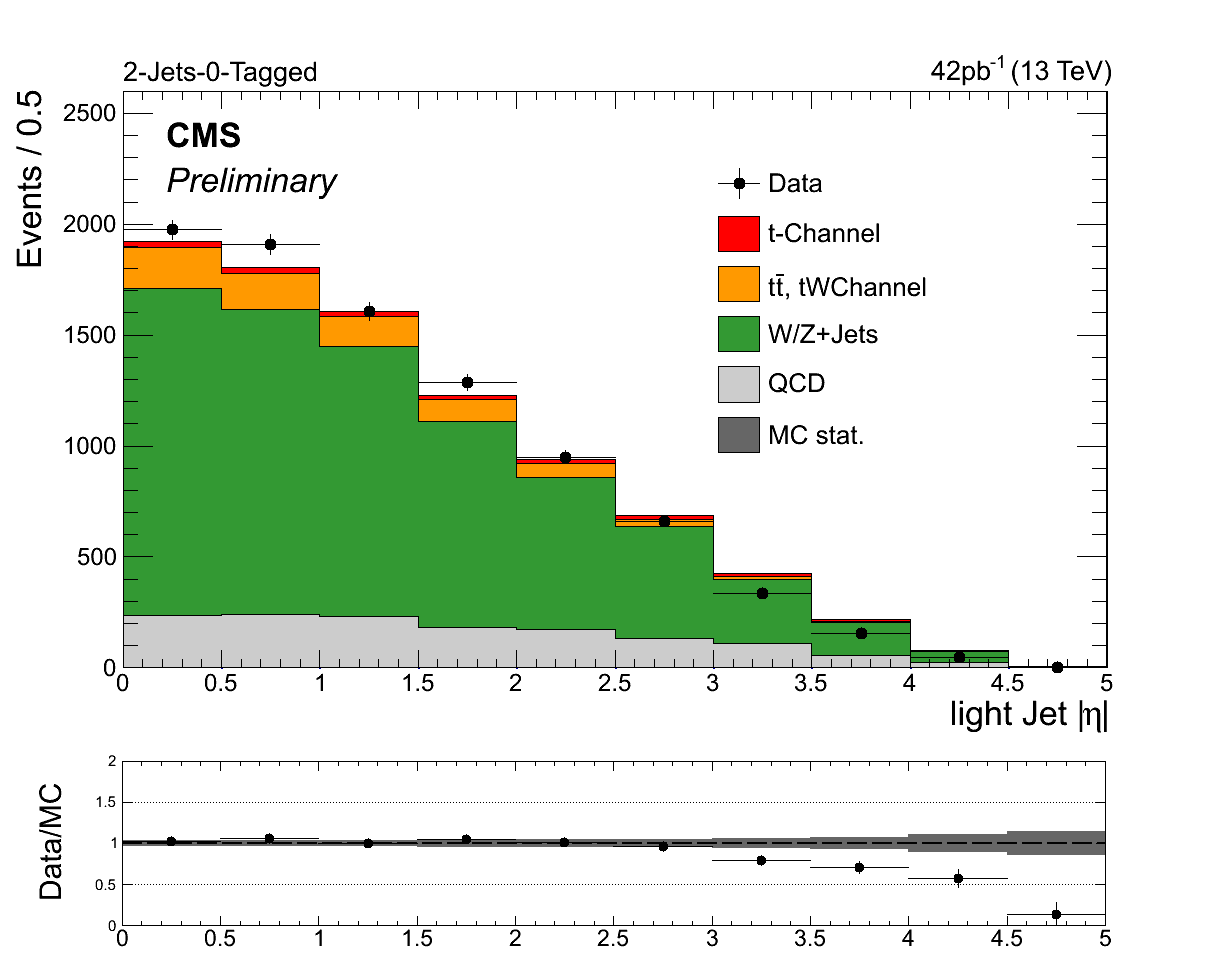
\includegraphics[width=0.45\textwidth,height=0.4\textwidth]{figures/2J0T/Sep8/lightJetEta.png}
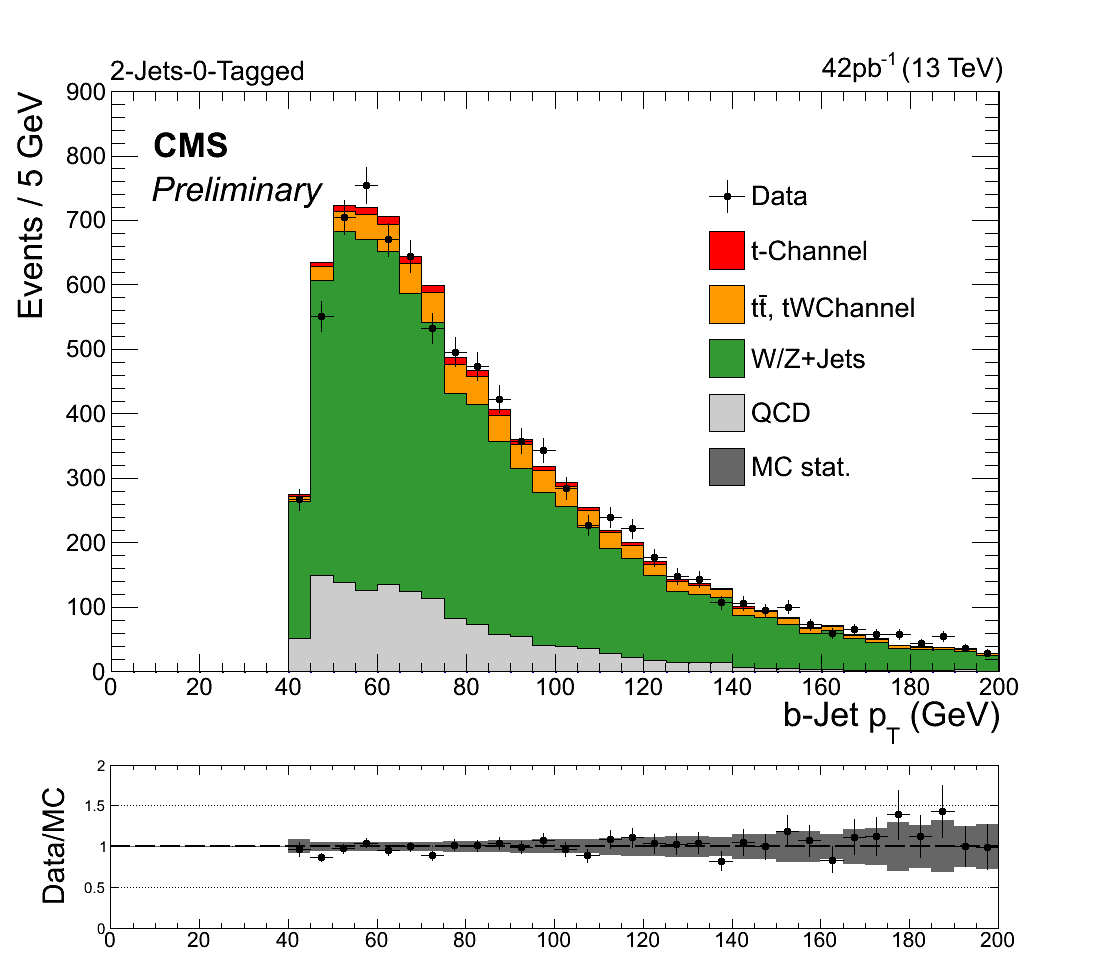
\includegraphics[width=0.45\textwidth,height=0.4\textwidth]{figures/2J0T/Sep8/bJetPt.png}
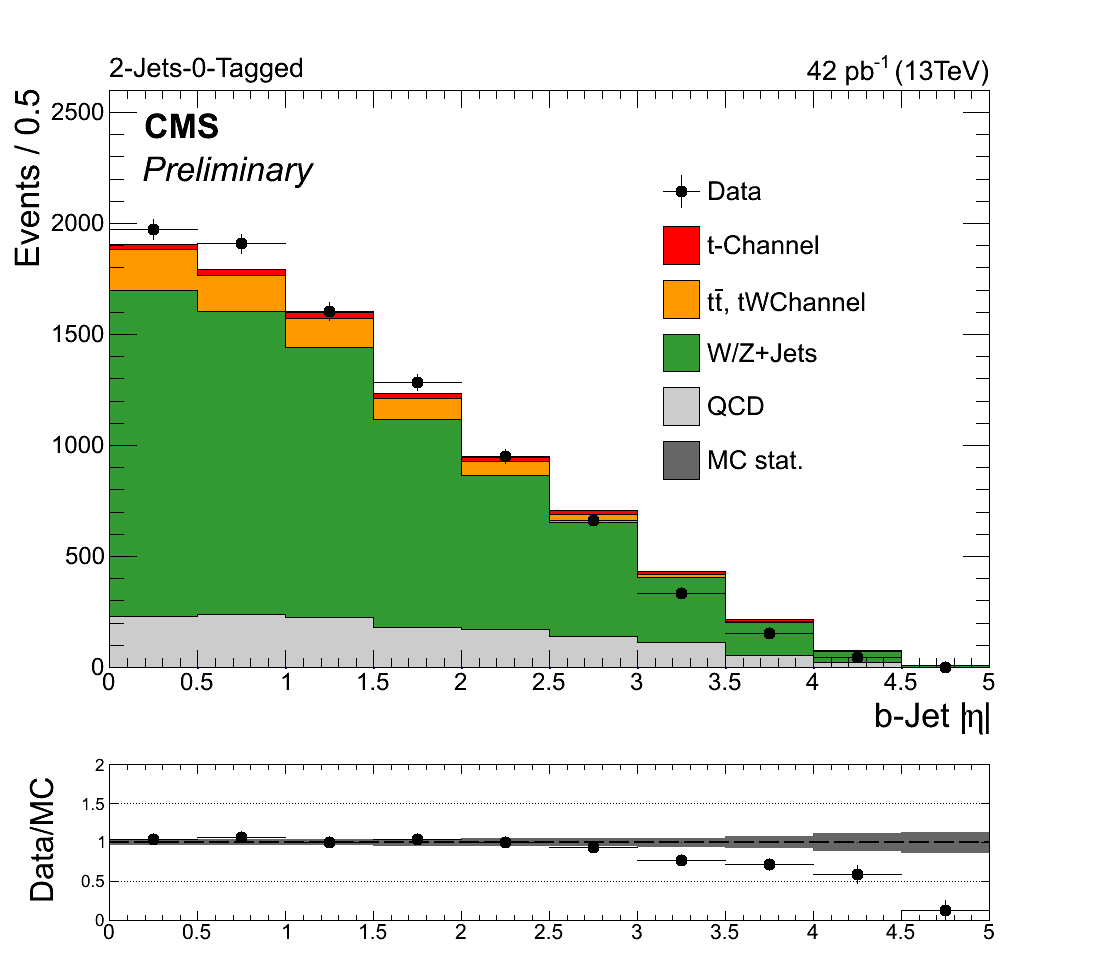
\includegraphics[width=0.45\textwidth,height=0.4\textwidth]{figures/2J0T/Sep8/bJetEta.png}\hfill
\caption{\label{fig:Jets2J0T}p$_{T}$ (left) and absolute value of $\eta$ (right) distributions of the "light" jet (upper row) and the "b" jet (lower row) in the 2J0T region. As this is the 0T region, the "b" jet refers to the jet with higher $p_{\mathrm{T}}$ and the "light" jet to the other jet.}
\end{center}
\end{figure}


\begin{figure}[hbpt]
\begin{center}
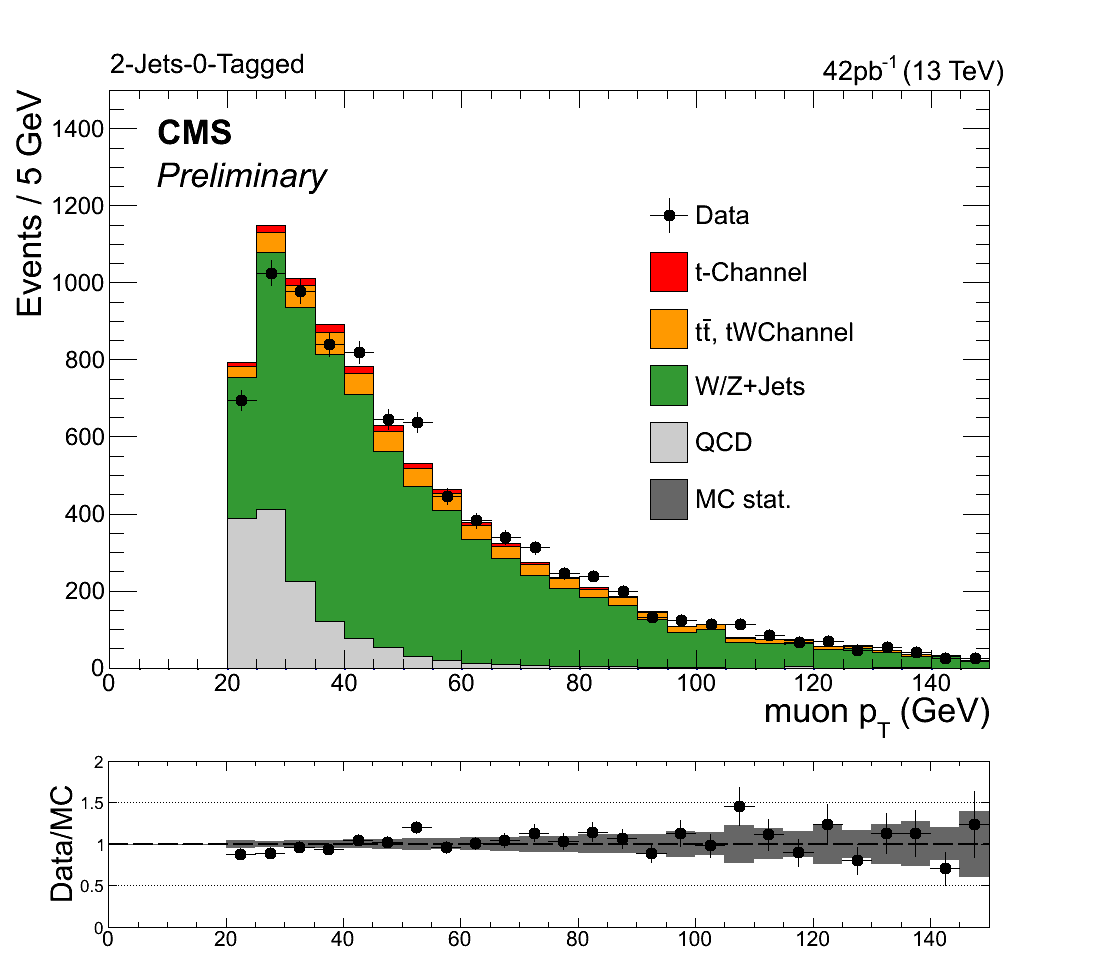
\includegraphics[width=0.45\textwidth,height=0.4\textwidth]{figures/2J0T/Sep8/muPt.png}
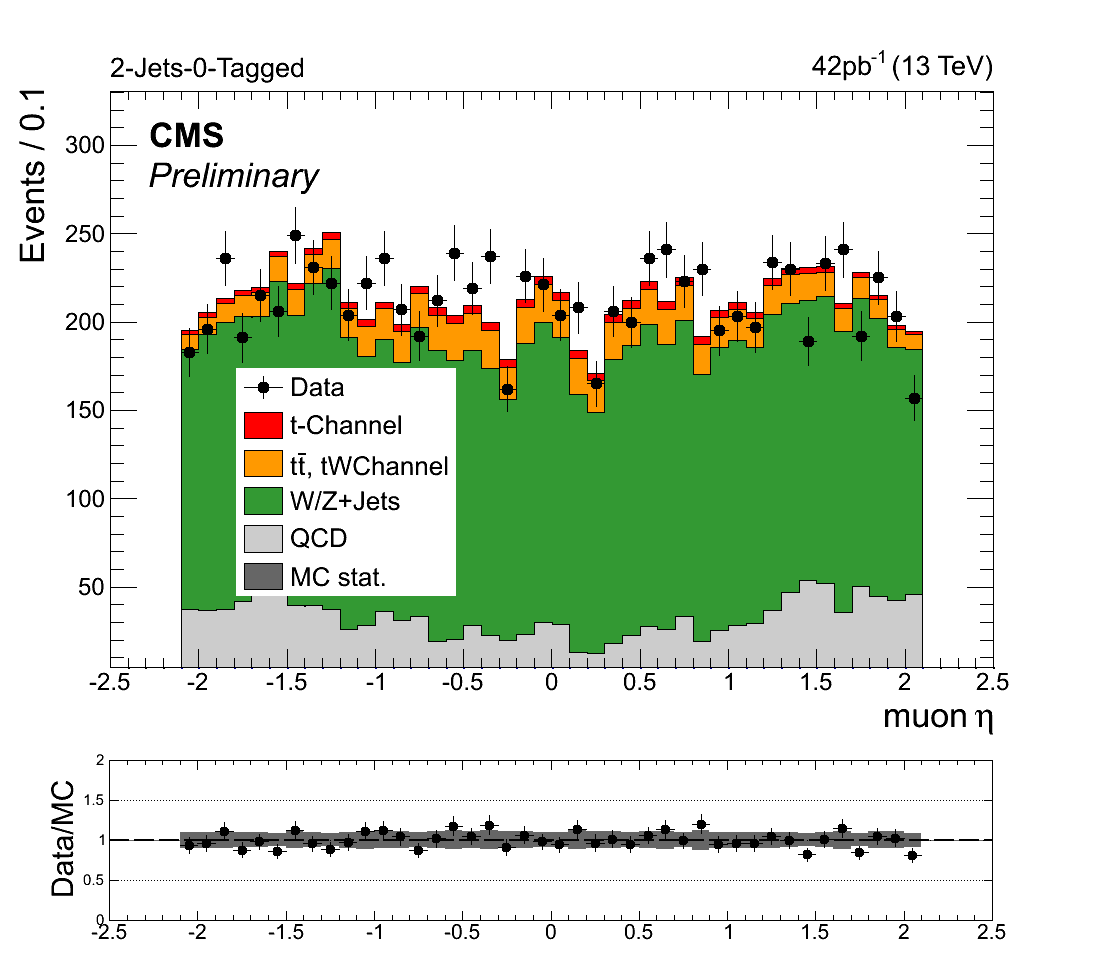
\includegraphics[width=0.45\textwidth,height=0.4\textwidth]{figures/2J0T/Sep8/muEta.png}
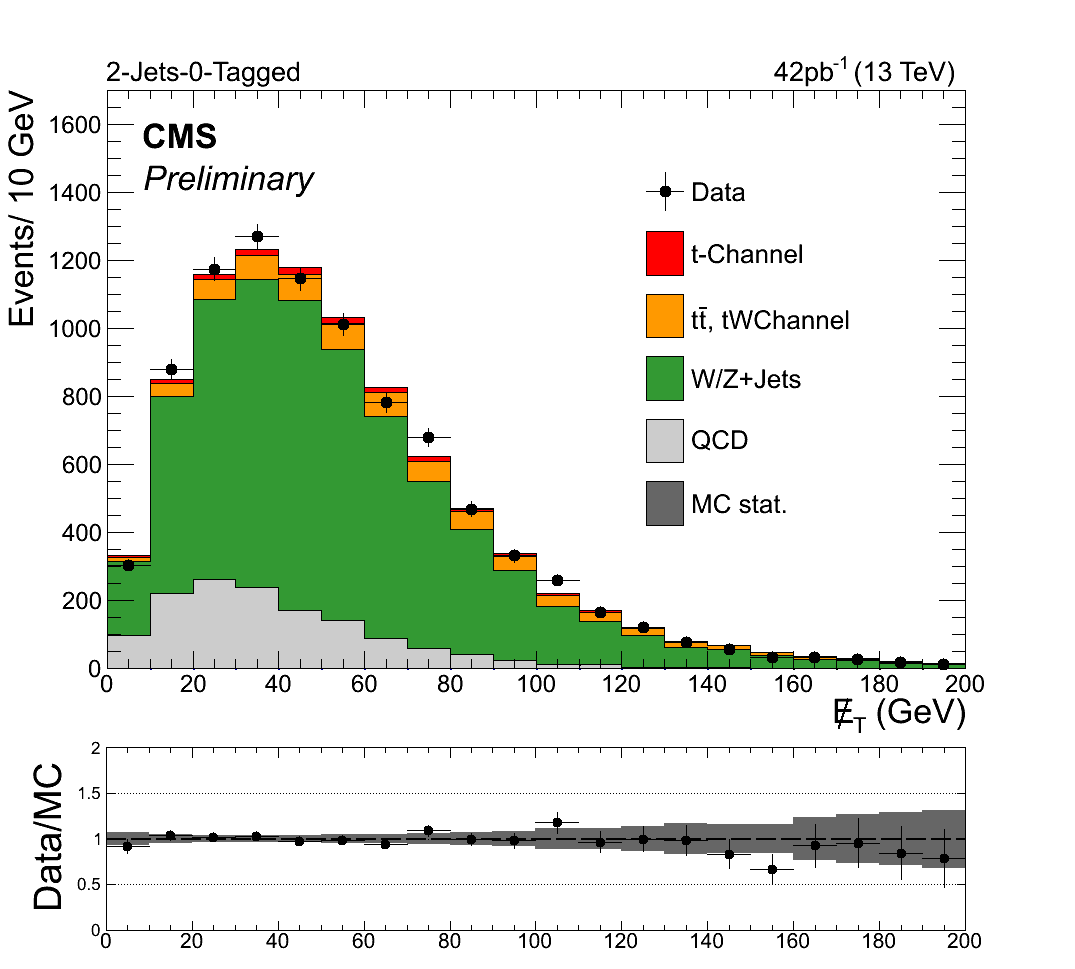
\includegraphics[width=0.45\textwidth,height=0.4\textwidth]{figures/2J0T/Sep8/metPt.png}
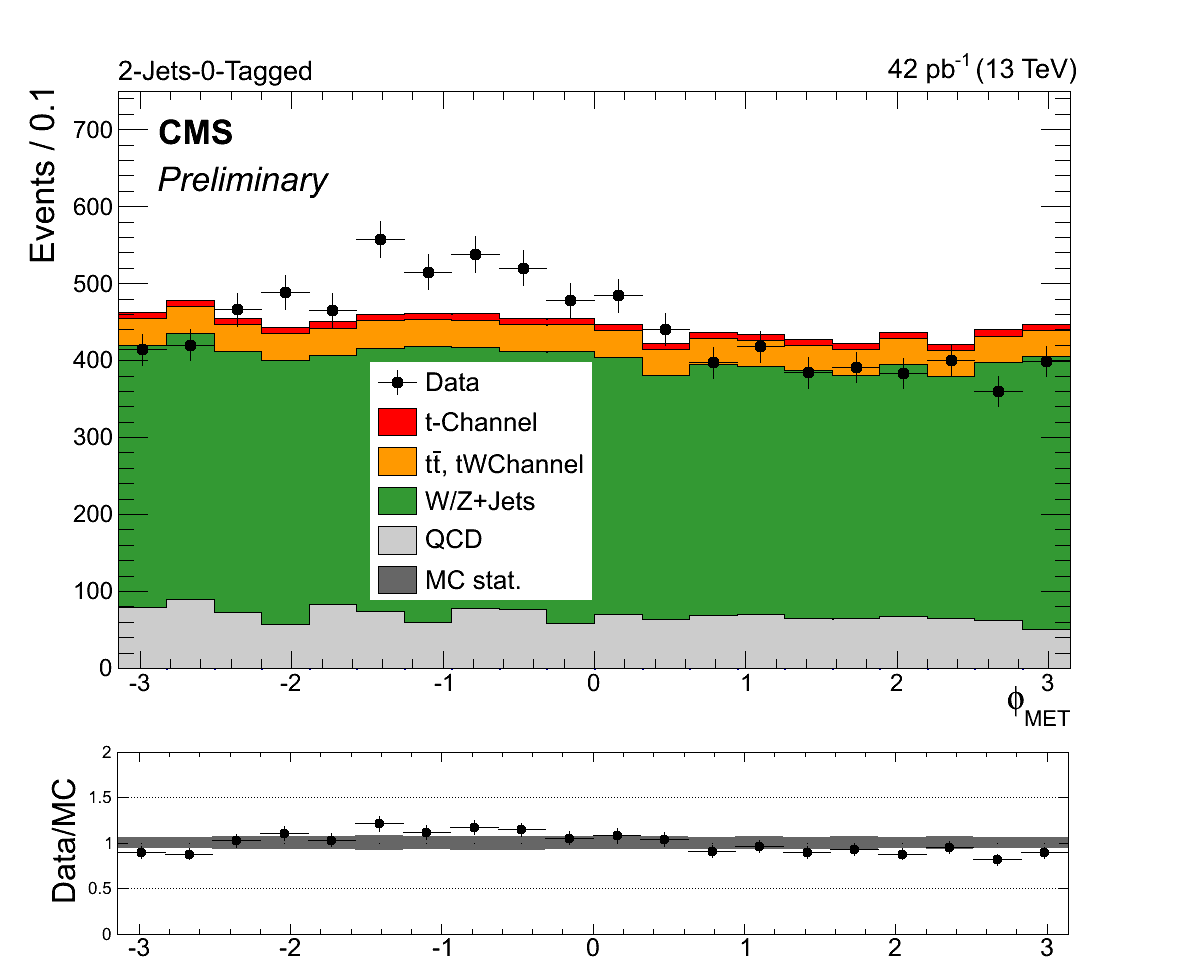
\includegraphics[width=0.45\textwidth,height=0.4\textwidth]{figures/2J0T/Sep8/metPhi.png}
\includegraphics[width=0.45\textwidth,height=0.4\textwidth]{figures/2J0T/Sep8/mtW.png}\hfill
\caption{\label{fig:Mu_MET_2J0T} Distributions of muon p$_{T}$ (upper left) and $\eta$ (upper right) in the 2J0T region and \met (middle left) and \met-$\phi$ (middle right) and \mT (bottom) in the 2J0T region.}
\end{center}
\end{figure}





%\begin{figure}[hbpt]
%\begin{center}
%\includegraphics[width=0.45\textwidth]{figures/2J0T/2j0t_ljet_abseta_qcdnone.png}
%\caption{\label{fig:etajprime2J0T}$\eta_{j'}$ distribution in 2J0T}
%\end{center}
%\end{figure}

\clearpage

\subsection{3J2T Control region}

The 3J2T control region is dominated by \ttbar~ events. In order to test the \ttbar~simulation again the distributions of several kinematic variables from simulation are compared to the distributions from data. 


\begin{figure}[hbpt]
\begin{center}
\includegraphics[width=6.5cm]{figures/3J2T/3j2t_muPt.pdf}
\includegraphics[width=6.5cm]{figures/3J2T/3j2t_mueta.pdf}
\includegraphics[width=6.5cm]{figures/3J2T/3j2t_MET.pdf}
\includegraphics[width=6.5cm]{figures/3J2T/3j2t_mt.pdf}\hfill
\caption{\label{fig:Mu_MET_3J1T} Distributions of muon p$_{T}$ (upper left) and $\eta$ (upper right) and \met (lower left) and \mt (lower right) in the 3J2T region.}
\end{center}
\end{figure}




\begin{figure}[hbpt]
\begin{center}
\includegraphics[width=6.5cm]{figures/3J2T/3j2t_ptjp.pdf}
\includegraphics[width=6.5cm]{figures/3J2T/3j2t_etajp.pdf}
\includegraphics[width=6.5cm]{figures/3J2T/3j2t_bpt.pdf}
\includegraphics[width=6.5cm]{figures/3J2T/3j2t_beta.pdf}\hfill
\caption{\label{fig:Jets3J2T}p$_{T}$ (left) and $\eta$ (right) distributions of the non-tagged jet (upper row) and the b-tagged jet with the highest CSV-value in each event (lower row) in the 3J2T region.}
\end{center}
\end{figure}

\clearpage

%\section{W+light flavour jets control sample}
%\label{sec:2J0T}
%\label{sec:WJets}
%\label{sec:wjets}
%This section describes a \wjets enriched control sample, a validation of the
analysis variables in this region and the addition of extra cuts introduced
to increase the robustness of this analysis against pile up effects.

The \wjets enriched sample is defined requiring exactly 2 jets defined as in Sec. ~\ref{sec:selection},
but vetoing any b-tagged jet. This sample is also referred to as the 2J0T sample.

\begin{figure}[hbpt]
\begin{center}
\caption{Muon p$_{\rm{T}}$ (left) \& $\eta$ (right) distributions in 2J0T}
\includegraphics[width=6.5cm]{figures/2J0T/muPt.png}
\includegraphics[width=6.5cm]{figures/2J0T/muEta.png}\hfill
\end{center}
\end{figure}
\\
\begin{figure}[hbpt]
\begin{center}
\caption{Leading jet p$_{\rm{T}}$ (left) \& $\eta$ (right) distributions in 2J0T}
\includegraphics[width=6.5cm]{figures/2J0T/leadJetPt.png}
\includegraphics[width=6.5cm]{figures/2J0T/leadJetEta.png}\hfill
\end{center}
\end{figure}
\\
\begin{figure}[hbpt]
\begin{center}
\caption{Sub-leading jet p$_{\rm{T}}$ (left) \& $\eta$ (right) distributions in 2J0T}
\includegraphics[width=6.5cm]{figures/2J0T/secondJetPt.png}
\includegraphics[width=6.5cm]{figures/2J0T/secondJetEta.png}\hfill
\end{center}
\end{figure}

\begin{figure}[hbpt]
\begin{center}
\caption{ Missing E$_{\rm{T}}$ (left) \& m$_{T}$ (right) distributions in 2J0T}
\includegraphics[width=6.5cm]{figures/2J0T/metPt_0To200.png}
\includegraphics[width=6.5cm]{figures/2J0T/MtW_0To200.png}\hfill 
\end{center}
\end{figure}
\\
\begin{figure}[hbpt]
\begin{center}
\caption{Reconstructed Top Mass distribution in 2J0T}
\includegraphics[width=8.0cm]{figures/2J0T/mtop.png}\hfill
\end{center}
\end{figure}
\newpage  
%2Table \ref{tab:2J0T} shows the composition of this sample for muons and electrons. 
%
%\input{yieldTableWSample}
%
%Figure~\ref{fig:2J0TmtwMassMET} shows the W transverse mass distribution (a,b) and the \MET (c,d) for muons (a,c) and electrons (b,d).
%The most disagreement is located where most of the \qcd is located. The treatment of \qcd will be done in Sec~\ref{sec:qcd}, allowing to determine
%from data the \qcd yield.
%
%	\begin{figure}[h]
%	  \begin{center}
%	    \subfigure[]{
%	    \includegraphics[width=0.48\textwidth]{figures/2J_0T_noSyst_noQCDCut_mtwMass_MuStack.png}}
%	    \subfigure[]{
%	    \includegraphics[width=0.48\textwidth]{figures/2J_0T_noSyst_noQCDCut_mtwMass_EleStack.png}}\\
%	    \subfigure[]{
%	    \includegraphics[width=0.48\textwidth]{figures/2J_0T_noSyst_noQCDCut_metPt_MuStack.png}}
%	    \subfigure[]{
%	    \includegraphics[width=0.48\textwidth]{figures/2J_0T_noSyst_noQCDCut_metPt_EleStack.png}}\\
%	    \caption{\label{fig:2J0TmtwMassMET}{Distributions of \mtw (a,c), \met (c,d), in the 2 jets 0 tags sample for muons (a,c) and electrons (b,d).}}
%	  \end{center}
%	\end{figure}
%
%
%In the high \met or \mTW region, representing the qcd depleted region for both variables, we observe a better data-MC agreement in the \met, 
%especially in the electron channel. This motivates us to use the \met for our \qcd determination for electrons.
%
%Figure~\ref{fig:2J0TLepton} shows the lepton \pt and relative isolation after the \qcd rejection cut:
%
%	\begin{figure}[h]
%	  \begin{center}
%	    \subfigure[]{
%	    \includegraphics[width=0.48\textwidth]{figures/2J_0T_noSyst_leptonPt_MuStack.png}}
%	    \subfigure[]{
%	    \includegraphics[width=0.48\textwidth]{figures/2J_0T_noSyst_leptonDeltaCorrectedRelIso_MuStack.png}}\\
%	    \subfigure[]{
%	    \includegraphics[width=0.48\textwidth]{figures/2J_0T_noSyst_leptonPt_EleStack.png}}
%	    \subfigure[]{
%	    \includegraphics[width=0.48\textwidth]{figures/2J_0T_noSyst_leptonRhoCorrectedRelIso_EleStack.png}}\\
%	    \caption{\label{fig:2J0TLepton}{Distributions of \pt (a,b), relative isolation (c,b) in the muon (a,c) and electron (b,d) channel in the 2 jets 0 tags sample after the $\qcd$ cut.}}
%	  \end{center}
%	\end{figure}
%
%Finally, figure ~\ref{fig:2J0TcosthetaLepMET} shows the cosinus of the angle between the lepton and the \MET $cos(\Delta\Phi_{\mu,\MET})$ before (a,b) and after (c,d) the cut for qcd rejection. Such angle is the other component of \mTW besides lepton momentum and missing energy.
%
%	\begin{figure}[h]
%	  \begin{center}
%	    \subfigure[]{
%	    \includegraphics[width=0.48\textwidth]{figures/2J_0T_noSyst_noQCDCut_cosLepMetPhi_MuStack.png}}
%	    \subfigure[]{
%	    \includegraphics[width=0.48\textwidth]{figures/2J_0T_noSyst_noQCDCut_cosLepMetPhi_EleStack.png}}\\
%	    \subfigure[]{
%	    \includegraphics[width=0.48\textwidth]{figures/2J_0T_noSyst_cosLepMetPhi_MuStack.png}}
%	    \subfigure[]{
%	    \includegraphics[width=0.48\textwidth]{figures/2J_0T_noSyst_cosLepMetPhi_EleStack.png}}\\
%	    \caption{\label{fig:2J0TcosthetaLepMET}{Distributions of the cosinus of the angle between the lepton and the \met for muons (a) and electrons(b).}}
%	  \end{center}
%	\end{figure}
%
%Another important variable for the analysis is the reconstructed top mass, for which a jet has to be
%chosen for the top quark decay ansatz. In this sample, the jet with highest value of the track counting
%high purity algorithm is chosen. The reconstructed top mass is shown in figure ~\ref{fig:2J0TtopMass}(a,b).
%
%
%	\begin{figure}[h]
%	  \begin{center}
%	    \subfigure[]{
%	    \includegraphics[width=0.48\textwidth]{figures/2J_0T_noSyst_topMass_MuStack.png}}
%	    \subfigure[]{
%	    \includegraphics[width=0.48\textwidth]{figures/2J_0T_noSyst_topMass_EleStack.png}}
%	    \caption{\label{fig:2J0TtopMass}{Distributions of \mt for muons (a) and electrons(b) in the 2 jets 0 tags sample.}}
%	  \end{center}
%	\end{figure}
%
%
%The pseudorapidity of the jets is a crucial variable for the strategy in this analysis. Fig. \ref{fig:2J0Teta} shows the pseudorapidity distribution 
%of the jet with the lowest value of b-discriminator (henceforth also referred to as ``light jet $\eta$''), while Fig. \ref{fig:2J0Teta_inclusive} 
%shows the pseudorapidity distribution of both jets (henceforth also referred to as ``inclusive jet $\eta$''), in both cases for muons (a) and electrons(b).
%
%	\begin{figure}[h]
%	  \begin{center}
%	    \subfigure[]{
%	    \includegraphics[width=0.48\textwidth]{figures/2J_0T_noSyst_etalj_MuStack.png}}
%	    \subfigure[]{
%	    \includegraphics[width=0.48\textwidth]{figures/2J_0T_noSyst_etalj_EleStack.png}}
%	    \caption{\label{fig:2J0Teta}{Pseudorapidity distributions of the jet with the lowest value of b-discriminator(``light jet $\eta$'') 
%	    in the 2 jets 0 tags sample for muons (a) and electrons (b)}}
%	  \end{center}
%	\end{figure}
%
%	\begin{figure}[h]
%	  \begin{center}
%	    \subfigure[]{
%	    \includegraphics[width=0.48\textwidth]{figures/2J_0T_noSyst_etalj_inclusiveMuStack.png}}
%	    \subfigure[]{
%	    \includegraphics[width=0.48\textwidth]{figures/2J_0T_noSyst_etalj_inclusiveEleStack.png}}
%	    \caption{\label{fig:2J0Teta_inclusive}{Pseudorapidity distributions of both jets in the event(``inclusive $\eta$'') 
%	    in the 2 jets 0 tags sample for muons (a) and electrons (b)}}
%	  \end{center}
%	\end{figure}
%
%Due to the different contributions of the u and d quarks proton $PDF$s,  \wjets processes are not symmetric as function of the lepton charge.
%This feature can be clearly seen in data: Fig. \ref{fig:2J0Tcharge} shows the lepton charge distribution in the sample for muons and electrons.
%There it can also be seen that the asymmetry in data tends to be different with respect to the prediction, thus in the signal extraction procedure the 
%$W$+ jets asymmetry shall be measured simultaneously to $R_{t-channel}$.
%
%Figures ~\ref{fig:2J0Teta_pm} and ~\ref{fig:2J0TtopMass_pm} show the distributions of light jet $\eta$ and \mt divided by charge.
%
%	\begin{figure}[h]
%	  \begin{center}
%	    \subfigure[]{
%	    \includegraphics[width=0.48\textwidth]{figures/charge_2J0T_Mu.pdf}}
%	    \subfigure[]{
%	    \includegraphics[width=0.48\textwidth]{figures/charge_2J0T_Ele.pdf}}
%	    \caption{\label{fig:2J0Tcharge}{Lepton charge in the 2 jets 0 tags sample for muons (a) and electrons (b)}}
%	  \end{center}
%	\end{figure}
%
%	\begin{figure}[h]
%	  \begin{center}
%	    \subfigure[]{
%	    \includegraphics[width=0.48\textwidth]{figures/2J_0T_noSyst_Plus_etalj_MuStack.png}}
%	    \subfigure[]{
%	    \includegraphics[width=0.48\textwidth]{figures/2J_0T_noSyst_Plus_etalj_EleStack.png}}\\
%	    \subfigure[]{
%	    \includegraphics[width=0.48\textwidth]{figures/2J_0T_noSyst_Minus_etalj_MuStack.png}}
%	    \subfigure[]{
%	    \includegraphics[width=0.48\textwidth]{figures/2J_0T_noSyst_Minus_etalj_EleStack.png}}\\
%	    \caption{\label{fig:2J0Teta_pm}{Pseudorapidity distributions of the light jet $\eta$ for positive(a,b) and negative (c,d) charge
%	    leptons in the 2 jets 0 tags sample for muons (a,c) and electrons (b,d)}}
%	  \end{center}
%	\end{figure}
%
%	\begin{figure}[h]
%	  \begin{center}
%	    \subfigure[]{
%	    \includegraphics[width=0.48\textwidth]{figures/2J_0T_noSyst_Plus_topMass_MuStack.png}}
%	    \subfigure[]{
%	    \includegraphics[width=0.48\textwidth]{figures/2J_0T_noSyst_Plus_topMass_EleStack.png}}\\
%	    \subfigure[]{
%	    \includegraphics[width=0.48\textwidth]{figures/2J_0T_noSyst_Minus_topMass_MuStack.png}}
%	    \subfigure[]{
%	    \includegraphics[width=0.48\textwidth]{figures/2J_0T_noSyst_Minus_topMass_EleStack.png}}\\
%	    \caption{\label{fig:2J0TtopMass_pm}{ \mt distributions for positive(a,b) and negative (c,d) charge leptons
%            in the 2 jets 0 tags sample for muons (a,c) and electrons (b,d) }}
%	  \end{center}
%	\end{figure}

%
%\section{\ttbar\ control samples}
%\label{sec:3JNT}
%\label{sec:TTBar}
%\label{sec:ttbar}
%%From figure ~\ref{fig:nbjetPresel} one can clearly see how 
This section describes the samples used to control the $\tt$ background.

The $\tt$ process is in general dominant in the 3-jets samples with 1 or more b-tags, and is also the main background to the $t$-channel in the 2-jets 1-tag category. Two meaningful $\ttbar$-enriched control samples are therefore the 3-jets, 1-tag and 3-jets, 2-tags samples.

%This sample is also enriched in W+heavy flavor jets.


%The highest TCHP tagged jet is used as candidate for the top reconstruction for both samples.
%Tables~\ref{tab:3J1T} and~\ref{tab:3J2T} show the yields for simulation and data in this control sample.
%One can notice a difference of O(10$\%$) in the 3-jets 1-tag category. This difference is partially cured taking into account the data 
%driven scale factors for the \wjets component of the background (see also appendix). 
%
%\input{yieldTable3J1T}
%\input{yieldTable3J2T}
%
%Figures ~\ref{fig:3JNTeta}, ~\ref{fig:3JNTtopMass} show the light jet $\eta$ and the \mt in those control samples for muons (a,c) and electrons (b,d).
%
%\begin{figure}[!h]
%\begin{center}
%\subfigure[]{
%\includegraphics[angle=0,width=0.48\textwidth]{figures/3J_1T_noSyst_etalj_MuStack.png}}
%	    \subfigure[]{
%\includegraphics[angle=0,width=0.48\textwidth]{figures/3J_1T_noSyst_etalj_EleStack.png}}\\
%\vskip -2ex
%\subfigure[]{
%\includegraphics[angle=0,width=0.48\textwidth]{figures/3J_2T_noSyst_etalj_MuStack.png}}
%	    \subfigure[]{
%\includegraphics[angle=0,width=0.48\textwidth]{figures/3J_2T_noSyst_etalj_EleStack.png}}\\
%\end{center}
%\caption{\label{fig:3JNTeta} distribution of the light jet $\eta$ in the $\ttbar$-enriched samples in the 3-jets and 1(a,b) or 2(c,d) tags, 
%muons (a,c) and electrons (b,d). }
%%(a,c,e runs $\ge$ 166404, \lumiMu \invpb ) and electrons (b,d,f 166404 $\le$  runs $<$ \maxrun, \lumiEleValidation \invpb ) }
%\end{figure}
%
%\begin{figure}[!h]
%\begin{center}
%\subfigure[]{
%\includegraphics[angle=0,width=0.48\textwidth]{figures/3J_1T_noSyst_topMass_MuStack.png}}
%	    \subfigure[]{
%\includegraphics[angle=0,width=0.48\textwidth]{figures/3J_1T_noSyst_topMass_EleStack.png}}\\
%\vskip -2ex
%\subfigure[]{
%\includegraphics[angle=0,width=0.48\textwidth]{figures/3J_2T_noSyst_topMass_MuStack.png}}
%	    \subfigure[]{
%\includegraphics[angle=0,width=0.48\textwidth]{figures/3J_2T_noSyst_topMass_EleStack.png}}\\
%\end{center}
%\caption{\label{fig:3JNTtopMass} distribution of the \mt in the $\ttbar$-enriched samples in the 3-jets and 1(a,b) or 2(c,d) tags, 
%muons (a,c) and electrons (b,d). }
%%(a,c,e runs $\ge$ 166404, \lumiMu \invpb ) and electrons (b,d,f 166404 $\le$  runs $<$ \maxrun, \lumiEleValidation \invpb ) }
%\end{figure}
% 
%\ttbar backgrounds are expected to be symmetric, and this can be checked in data on those control samples. Figure \ref{fig:3JNTcharge} shows the lepton charge normalized to the data yield obtained for the sake of displaying this feature.
%
%\begin{figure}[!h]
%\begin{center}
%\subfigure[]{
%\includegraphics[angle=0,width=0.48\textwidth]{figures/3J_1T_noSyst_DDNorm_charge_MuStack.png}}
%	    \subfigure[]{
%\includegraphics[angle=0,width=0.48\textwidth]{figures/3J_1T_noSyst_DDNorm_charge_EleStack.png}}\\
%\vskip -2ex
%\subfigure[]{
%\includegraphics[angle=0,width=0.48\textwidth]{figures/3J_2T_noSyst_DDNorm_charge_MuStack.png}}
%	    \subfigure[]{
%\includegraphics[angle=0,width=0.48\textwidth]{figures/3J_2T_noSyst_DDNorm_charge_EleStack.png}}\\
%\end{center}
%\caption{\label{fig:3JNTcharge} lepton charge in the 3-jets and 1(a,b) or 2(c,d) tags, 
%muons (a,c) and electrons (b,d). Simulation normalized to the data yield.}
%%(a,c,e runs $\ge$ 166404, \lumiMu \invpb ) and electrons (b,d,f 166404 $\le$  runs $<$ \maxrun, \lumiEleValidation \invpb ) }
%\end{figure}
%
%Figg. ~\ref{fig:3JNTeta_pm} and  ~\ref{fig:3JNTtopMass_pm} show the behavior of the light jet $\eta$ and of the reconstructed top mass $\topMass$ for positive and negative charge leptons.
%
%\begin{figure}[!h]
%\begin{center}
%\subfigure[]{
%\includegraphics[angle=0,width=0.48\textwidth]{figures/3J_1T_noSyst_Plus_etalj_MuStack.png}}
%	    \subfigure[]{
%\includegraphics[angle=0,width=0.48\textwidth]{figures/3J_1T_noSyst_Plus_etalj_EleStack.png}}\\
%\subfigure[]{
%\includegraphics[angle=0,width=0.48\textwidth]{figures/3J_1T_noSyst_Minus_etalj_MuStack.png}}
%	    \subfigure[]{
%\includegraphics[angle=0,width=0.48\textwidth]{figures/3J_1T_noSyst_Minus_etalj_EleStack.png}}\\
%\vskip -2ex
%\subfigure[]{
%\includegraphics[angle=0,width=0.48\textwidth]{figures/3J_2T_noSyst_Plus_etalj_MuStack.png}}
%	    \subfigure[]{
%\includegraphics[angle=0,width=0.48\textwidth]{figures/3J_2T_noSyst_Plus_etalj_EleStack.png}}\\
%\subfigure[]{
%\includegraphics[angle=0,width=0.48\textwidth]{figures/3J_2T_noSyst_Minus_etalj_MuStack.png}}
%	    \subfigure[]{
%\includegraphics[angle=0,width=0.48\textwidth]{figures/3J_2T_noSyst_Minus_etalj_EleStack.png}}\\
%\end{center}
%\caption{\label{fig:3JNTeta_pm} light jet $\eta$ in the 3-jets and 1(a-d) or 2(e-h) tags, 
%muons (a,c,e,g) and electrons (b,d,f,h), for positive (a,b,e,f) and negative (c,d,g,h) charge.}
%%(a,c,e runs $\ge$ 166404, \lumiMu \invpb ) and electrons (b,d,f 166404 $\le$  runs $<$ \maxrun, \lumiEleValidation \invpb ) }
%\end{figure}
%
%%Figures ~\ref{fig:3JNTtopMass}(a),(b) show the distribution of the top mass and the peak which is mostly populated by to semi-leptonic events where
%%the b-tagged jet coming from the same top quark as the lepton is chosen, similarly to what happens with single top $t$-channel events.
%\begin{figure}[!h]
%\begin{center}
%
%\subfigure[]{
%\includegraphics[angle=0,width=0.48\textwidth]{figures/3J_1T_noSyst_Plus_topMass_MuStack.png}}
% \subfigure[]{
%\includegraphics[angle=0,width=0.48\textwidth]{figures/3J_1T_noSyst_Plus_topMass_EleStack.png}}\\
%\subfigure[]{
%\includegraphics[angle=0,width=0.48\textwidth]{figures/3J_1T_noSyst_Minus_topMass_MuStack.png}}
% \subfigure[]{
%\includegraphics[angle=0,width=0.48\textwidth]{figures/3J_1T_noSyst_Minus_topMass_EleStack.png}}\\
%\vskip -2ex
%\subfigure[]{
%\includegraphics[angle=0,width=0.48\textwidth]{figures/3J_2T_noSyst_Plus_topMass_MuStack.png}}
% \subfigure[]{
%\includegraphics[angle=0,width=0.48\textwidth]{figures/3J_2T_noSyst_Plus_topMass_EleStack.png}}\\
%\subfigure[]{
%\includegraphics[angle=0,width=0.48\textwidth]{figures/3J_2T_noSyst_Minus_topMass_MuStack.png}}
% \subfigure[]{
%\includegraphics[angle=0,width=0.48\textwidth]{figures/3J_2T_noSyst_Minus_topMass_EleStack.png}}\\
%\end{center}
%\caption{\label{fig:3JNTtopMass_pm} \mt in the 3-jets and 1(a-d) or 2(e-h) tags, muons (a,c,e,g) and electrons (b,d,f,h), for positive (a,b,e,f) and negative (c,d,g,h) charge.}
%%(a,c,e runs $\ge$ 166404, \lumiMu \invpb ) and electrons (b,d,f 166404 $\le$  runs $<$ \maxrun, \lumiEleValidation \invpb ) }
%\end{figure}
%
%%Figure ~\ref{fig:eta3J2TSRSB} shows the agreement in the signal and sideband region for \etalj in the 3-jets, 2-tags sample for the muons and elecrtons.
%
%A reweighting function is extracted from the signal and sideband regions of the 3-jets 2-tags sample. This extraction is performed exactly as in  Refs.~\cite{AN-12-273,CMS-PAS-TOP-12-011}. The extracted function is then applied to the ~\tt~ Monte Carlo distribution in the signal region. 
%Since the ~\tt~ sample is symmetric as a function of the charge, we perform the extraction before separating by charge.
%Figure ~\ref{fig:3J2TetaChargeComparison} shows that, according to simulation, the top model for light jet $\eta$ is independent of the charge of the lepton.
%%This allows to reduce the dependancy on the statistical fluctuations in the 3-jets 2-tags sample.
%
%\begin{figure}[!h]
%\begin{center}
%\subfigure[]{
%\includegraphics[angle=0,width=0.48\textwidth]{figures/ttbar3J2TEtaChargeComparisonMu.png}}
%	    \subfigure[]{
%\includegraphics[angle=0,width=0.48\textwidth]{figures/ttbar3J2TEtaChargeComparisonEle.png}}
%\vskip -2ex
%\end{center}
%\caption{\label{fig:3J2TetaChargeComparison} findme Comparison between the light jet $\eta$ distributions of samples with positive and negative leptons in the $\ttbar$-enriched samples with 3-jets 2-tags sample for muons (a) and electrons (b). }
%\end{figure}
%
%

%
%To cope with any possible modeling effect, we get a reweighting function for the overall $\eta$ distribution
% of the light jet taking the bin-by-bin difference between data and MC. We use this as a systematic uncertainty on the \ttbar\ model for the time being.
%\begin{figure}[!h]
%\begin{center}
%\subfigure[]{
%\includegraphics[angle=0,width=0.48\textwidth]{figures/ttbar/3J_2T_noSyst_etalj_SRMuStack.png}}
%	    \subfigure[]{
%\includegraphics[angle=0,width=0.48\textwidth]{figures/ttbar/3J_2T_noSyst_etalj_SBMuStack.png}}
%\vskip -2ex
%\end{center}
%\vskip -2ex
%\caption{\label{fig:eta3J2TSRSB} Distribution of $|\eta|$ of the jet with the lowest value of b-discriminator
% in the $\ttbar$-enriched samples with 3-jets 2-tags sample inside(a) and outside(b) the 
%$130<\topMass<220$ region. }
%\end{figure}
%
%An extraction procedure is applied in a similar way to what is done in ~\ref{}
%
%
%
%
%
%To extract a reweighting function in the 2-jets 1-tag category, where we intend to perform the signal extraction, we
%first compare in Figure ~\ref{fig:3JNTVS2J1T} shows that the light jet $\eta$ in the 3-jets 1-,and 2-tags categories
%to the one from the 2-jets 1-tag, finding that the 3-jets 2-tag region displays a similar $\eta$ distribution as the one in the 2-jet 1-tag
%sample.
%
%\begin{figure}[!h]
%\begin{center}
%\subfigure[]{
%\includegraphics[angle=0,width=0.48\textwidth]{figures/ttbar/3JNTvs2J1TSR.pdf}}
%	    \subfigure[]{
%\includegraphics[angle=0,width=0.48\textwidth]{figures/ttbar/3JNTvs2J1TSB.pdf}}
%\vskip -2ex
%\end{center}
%\vskip -2ex
%\caption{\label{fig:3JNTVS2J1T} comparison of the MC distribution of $|\eta|$ of the jet with the lowest value of b-discriminator
% in the $\ttbar$-enriched samples with 3-jets N(=1,2) tags  vs the same distribution for the 2-jets 1-tag category for \ttbar\ events inside(a) and outside(b) the 
%$130<\topMass<220$ region. }
%\end{figure}
%
%A reweighting function is extracted, taking the difference in shape between data and expectation, and it is shown 
%in Figure ~\ref{fig:ReweightingFunction} in the Signal(a) and Sideband(b) regions, with the corresponding statistical 
%uncertainties due to data. This does not take into account the MC statistics, which in particular for the signal 
%is crucial in the high $|\eta|$ region of this sample.
%However, such function is therefore applied to the MC distribution in the 2-jets 1-tag region, 
%avoiding the region above $|\etalj| >2.5$ for two reasons: the statistical fluctuations
%in this region significantly affect the shape extraction (see Fig.~\ref{fig:ReweightingFunction})
% and the signal contamination in this region is non negligible (see Fig.~\ref{fig:eta3J2TSRSB}),
%therefore would require a more complicated simultaneous fit to be dealt with effectively.
%
%
%\begin{figure}[!h]
%\begin{center}
%\subfigure[]{
%\includegraphics[angle=0,width=0.48\textwidth]{figures/ttbar/RemodelSR.png}}
%	    \subfigure[]{
%\includegraphics[angle=0,width=0.48\textwidth]{figures/ttbar/RemodelSB.png}}
%\vskip -2ex
%\end{center}
%\vskip -2ex
%\caption{\label{fig:ReweightingFunction} comparison of the MC distribution of $|\eta|$ of the jet with the lowest value of b-discriminator
% in the $\ttbar$-enriched samples with 3-jets N(=1,2) tags  vs the same distribution for the 2-jets 1-tag category for \ttbar\ events inside(a) and outside(b) the 
%$130<\topMass<220$ region. }
%\end{figure}

%Figure ~\ref{fig:3JNTPUZoomMass} shows how the light jet $\eta$ distributions are modified applying a cut in the reconstructed top mass $130 < \topMass < 220$,
%focusing on the $|\eta|>2 $ region.
%From those plots finds out that actually there is an excess of data with respect to MC in the top mass window (a,b), while there is a deficit in the top mass sideband (c,d).
%
%
%\end{figure}
%\begin{figure}[!h]
%\begin{center}
%	    \subfigure[]{
%\includegraphics[angle=0,width=0.48\textwidth]{figures/ttbar/3J_1TtopMassNoPU22TAfterCutsMuStack.png}}
%	    \subfigure[]{
%\includegraphics[angle=0,width=0.48\textwidth]{figures/ttbar/3J_2TtopMassNoPU22TAfterCutsMuStack.png}}
%\vskip -2ex	   
%  \subfigure[]{
%\includegraphics[angle=0,width=0.48\textwidth]{figures/ttbar/3J_1TtopMassNoPU22TAfterCutsMuStack.png}}
%	    \subfigure[]{
%\includegraphics[angle=0,width=0.48\textwidth]{figures/ttbar/3J_2TtopMassNoPU22TAfterCutsMuStack.png}}
%\end{center}
%\vskip -2ex
%\caption{\label{fig:3JNTPUZoomMass} distribution of the light jet $\eta$ in the window $130<\topMass<220$ (a,b) 
%and outside (c,d) in the $\ttbar$-enriched samples with 3-jets and 1(a,c) or 2(b,d) tags. }
%\end{figure}
%
%
%The ratio of events in the signal and sideband region depends on pile up , as it is shown in table ~\ref{tab:SRSBVSPU}. 
%
%Increasing the cut on the $RMS$ of the forward jet reduces the data-mc discrepancy, 
%but does not solve the problem entirely. 
%Table ~\ref{tab:SRSBVSRMS} shows the ratio of events inside and outside the top mass region
%$130 < \topMass < 220$ as function of the $RMS$ of the forward jet.
%
%%//Figure ~\ref{fig:3J2T}

%Where the shape for the qcd variables is extracted from the anti-isolated sample. 
%Table~\ref{tab:tt_control_KSTests} reportes the KS $p$-values for the data-simulation
%comparison of the $\costhetalj$, $\etalj$, and $\topMass$ distributions. 
%Fig.~\ref{fig:tt_control_topMass_TChan_vs_TTBar} shows that the $\topMass$ 
%distribution is similiar between $\ttbar$ and signal for the
%cases where the correct b-tagged jet is taken for reconstruction of the top.

% \begin{table}
% \begin{center}
%   \begin{tabular}{ |l|c|c| }
%  \hline
% Process/Observable  & KS(shape only) data-mc: muon & electron   \\
% \hline
% \etalj            & FIXME & FIXME\\
% \topMass          & 0.85 & 0.90  \\
% \costhetalj       & FIXME & FIXME\\
% \hline
% \end{tabular}
%   \end{center}
% \caption{ KS tests comparing the shapes of the \topMass }%discriminating variables from different samples}
% \label{tab:tt_control_KSTests}
%   \end{table}

%\begin{figure}[!h]
%\begin{center}
%	    \subfigure[]{
%\includegraphics[angle=0,width=0.48\textwidth]{figures/topMass_WSample_noSyst_MuStack.pdf}
%}
%\end{center}
%\vskip -2ex
%\caption{\label{fig:tt_control_topMass_TChan_vs_TTBar} Distribution of $\topMass$ in the $\ttbar$-enriched sample 
%for $t$-channel signal and $\ttbar$ events, requiring that the b jet used to reconstruct
%$\topMass$ is the one from top decay. Left: muons, right: electrons. FIXME}
%\end{figure}


%The shape extraction procedure is the following: $W+$light shape is obtained subtracting the contributions of all other channels from data in the following way: QCD shapes are taken from anti-isolated samples, qcd yields are taken from the fit to mtw and extrapolated after the cut to $M_T$, all other channels are taken from Monte Carlo.


\section{Modelling and estimation of the QCD background}
\label{sec:QCD}
\label{sec:qcd}
 The production of multijets through QCD processes has a huge cross section. On the other hand, only a small fraction of these events mimics the lepton+jets final state of the applied event selection and the selection efficiency for QCD multijet events is therefore tiny. The combination of huge cross section and tiny selection efficiency would require the generation of extremely large MC samples for this process in order to produce sufficient events that survive the event selection to guarantee a proper QCD modelling with decent statistics in the signal region.
 An alternative way of modelling QCD is to define sideband regions in data that are enriched in QCD events and take the distributions of the relevant kinematic variables directly from these data. In the following subsections we describe the definition of the QCD enriched sideband regions and the estimation of the QCD contribution to the signal region by means of a fit to a discriminiating variable. As the number of available events is larger in the 2J0T control region, we use this region for a proof of concept and detailed studies of the method which is then applied to the 2J1T region.

 
\subsection{Modelling of the QCD background in 2J0T}

The 2J0T control region is dominated by \QCD and W+light flavour jets events. The fraction of \QCD events can be significantly increased by inverting the isolation criterion for the muon ($\murelIso > 0.12$) in the 2J0T region. Figure~\ref{fig:qcdshape} shows for the transverse mass of the W boson a comparison between simulated QCD events in the isolated region ($\murelIso < 0.06$), in the anti-isolated region ($\murelIso > 0.12$), and in an intermediate region ($0.06 < \murelIso < 0.12$). Good agreement in the shapes of the distributions from the three orthogonal regions is found. Using samples of simulated events from all relevant signal and background processes the \QCD-purity of the anti-isolated  sideband region has been estimated to be 95\%. Therefore the small contributions from non-\QCD-processes can be neglected. 

\begin{figure}[hbpt]
\begin{center}
\includegraphics[width=0.45\textwidth]{figures/2J0T/Sep3/QCD_mtW_shape_Comparison.png}
\caption{\label{fig:qcdshape}Comparison of the m$_{T}$ shape for \QCD between isolated , moderately isolated  and anti-isolated region of 2J0T}
\end{center}
\end{figure}


\subsection{Estimation of the QCD-contribution in 2J0T}
\label{sec:qcd2J0T}
The transverse mass ($\mT$) of the $(\mu,\met)$ system provides good discrimination power between QCD and processes with prompt muons. An extended maximum likelihood fit with 2 parameters is performed to the $\mT$ distribution of in the 2J0T region. We assume that the \mT distribution in data F($\mT$) can be parametrized as 

\begin{center}
\begin{equation}
\label{eq:QCDFit}
F(\mT) = N_{\rm QCD} \cdot Q(\mT) + N_{\rm nonQCD} \cdot B(\mT)  ,
\end{equation}
\end{center}

where $Q(\mT)$ stands for the QCD \mT-template  taken from the anti-isolated region of 2J0T as described above, $B(\mT)$ is the non-QCD $\mT$-template obtained by summing up 
the simulated contributions from all other processes with prompt muons in the isolated region according to their predicted cross section. Both templates, $Q(\mT)$  and $B(\mT)$ are normalized to an integral of 1.0. The fit parameter $N_{\rm QCD}$ denotes the number of QCD events and $N_{\rm nonQCD}$ represents the total number of non-QCD events. The $N_{\rm QCD}$ and $N_{\rm nonQCD}$ parameters are allowed to float during the fit to the \mT distribution performed as shown in Figure~\ref{fig:qcdFit1} and ~\ref{fig:qcdFit2}.\\   
 The entire range of the \mT-distribution is fitted. From the resulting \QCD yield we extrapolate the \QCD-contribution to the signal region ($\mt > 50\,$\GeV) by calculating the integral of the \mT-distribution from \QCD normalized to the fit-result from $\mT = 50\,$\GeV to infinity.\\
 The QCD \mT-template is derived from data in the anti-isolated sideband region ($\murelIso > 0.12$), as described above, while the actual fit is performed in the signal region ($\murelIso < 0.06$). 

As a further cross check also an unbinned fit is performed. The fitted (and extrapolated) yields from the different types of fits to $\mT$ are summarized in Table~\ref{tab:QCDFitSF1}. Overall a good agreement between the different fits can be observed. A fit based on missing transverse energy instead of $\mT$ can be found in Appendix~\ref{app:METFit_2J0T}.


\begin{figure}[hbpt]
\begin{center}
\includegraphics[width=0.45\textwidth]{figures/2J0T/Sep8/BinnedFit_QCD_MC.png}
\includegraphics[width=0.45\textwidth]{figures/2J0T/Sep8/BinnedFit_QCD_DD.png}\hfill
%\includegraphics[width=0.45\textwidth]{figures/2J0T/Data_BinnedFit_QCD_DD.png}
\caption{\label{fig:qcdFit1}Post fit distribution of $\mT$ for binned fit where QCD shape is taken from MC (left) and data-driven (right) }
\end{center}
\end{figure}

\begin{figure}[hbpt]
\begin{center}
\includegraphics[width=0.6\textwidth]{figures/2J0T/Sep8/UnbinnedFit_QCD.png}
\caption{\label{fig:qcdFit2}Post fit distribution of $\mT$ for unbinned fit}
\end{center}
\end{figure}




\begin{table}
\begin{center}
\caption{QCD estimation in the 2J0T region}
\label{tab:QCDFitSF1}
\begin{tabular}{|c|c|c|c|c|c|}
\hline
Variable & Fit Type & QCD shape & Process & Fitted Yield & Extrapolated Yield\\
 & & & & (full range) & ($\mT>50$GeV) \\
\hline 
\multirow{6}{*}{\mT} & \multirow{2}{*}{Unbinned} & \multirow{2}{*}{Parametric} & QCD & 1510$\pm$137 & 501$\pm$46 \\\cline{4-6}
 & & & nonQCD & 7301$\pm$157 & 4407$\pm$95 \\\cline{2-6}
 & \multirow{4}{*}{Binned} & \multirow{2}{*}{From MC} & QCD & 1662$\pm$138 & 547$\pm$46 \\\cline{4-6}
 & & & nonQCD & 7149$\pm$157 & 4291$\pm$94 \\\cline{3-6}																		
 & & \multirow{2}{*}{Data Driven} & QCD & 1378$\pm$121 & 342$\pm$30 \\\cline{4-6}
 & & & nonQCD & 7433$\pm$144 & 4462$\pm$86 \\\cline{3-6}						   
\hline 
%\multirow{4}{*}{\met} & \multirow{4}{*}{Binned}& \multirow{2}{*}{From MC} & QCD & 2216$\pm$118 & 461$\pm$25 \\\cline{4-6}
% & & & nonQCD & 5804$\pm$133 & 3092$\pm$71 \\\cline{3-6}
% & & \multirow{2}{*}{Data Driven} & QCD & 1615$\pm$90 & 174$\pm$10 \\\cline{4-6}
% & & & nonQCD & 6406$\pm$114 & 3413$\pm$61 \\\cline{3-6}
%\hline
\end{tabular}
\end{center}
\end{table}




\newpage
\subsection{Modelling of the QCD background in 2J1T}
\label{sec:qcd2J1T}
The same procedure (inverting the relative isolation of the muon) is applied to the 2J1T region after the full selection inside and outside the top quark mass window used for signal extraction defined. Figure~\ref{fig:qcdShapeComparison2J1TmtW} shows a comparison of the \mT distribution between simulated QCD events in the isolated ( $\PFrelIso < 0.06$) against the anti-isolated region ($\PFrelIso > 0.12$), and in the intermediate region ($0.06 < \PFrelIso < 0.12$) against the  anti-isolated region. Good agreement in the shapes of the distributions from the different regions considered is found. 

Using samples of simulated events from all relevant signal and background processes the \QCD of the anti-isolated region seems overwhelming, as Table~\ref{tab:QCDEstimation2J1T} and Figure~\ref{fig:sampleComparisonDifferentIsoRegions2J1TmtW} indicate. 


\begin{table}[h!] \begin{center}
\caption{QCD and nonQCD expectation in 2J1T region for \mylumi~pb$^{-1}$} \label{tab:QCDEstimation2J1T} \resizebox{\textwidth}{!}{\begin{tabular}{|l|l|l|c @{$\pm$} l|c @{$\pm$} l|c @{$\pm$} l|} \hline $m_{\ell\nu\mathrm{b}}$ range & Cut & Process & \multicolumn{2}{c|}{$\PFrelIso < 0.06$}  &  \multicolumn{2}{c|}{$0.06< \PFrelIso < 0.12$} &\multicolumn{2}{c|}{$\PFrelIso > 0.12$}\\ \hline
\multirow{4}{*}{inclusive} & \multirow{2}{*}{No Cut} & QCD & 204&14 & 194&14&534&23\\\cline{3-9} & & nonQCD & 520&7 & 75&3 &42&2\\\cline{2-9} & \multirow{2}{*}{$m_{T}\  \rm{of\  W} >$ 50 GeV} & QCD & 58&8 & 50&7\\\cline{3-7} & & nonQCD &355&6 & 52&2\\\cline{2-7} \hline

\multirow{4}{*}{outside window} & \multirow{2}{*}{No Cut} & QCD & 59&8 & 55&7&153&12\\\cline{3-9} & & nonQCD & 201&5 & 25&1.5 &12&1\\\cline{2-9} & \multirow{2}{*}{$m_{T}\  \rm{of\  W} >$ 50 GeV} & QCD & 11&3 & 19&4\\\cline{3-7} & & nonQCD &130&4 & 16&1.1\\\cline{2-7} \hline

\multirow{4}{*}{inside window} & \multirow{2}{*}{No Cut} & QCD & 145&12 & 138&11&381&20\\\cline{3-9} & & nonQCD & 335&5 & 51&2 &30&1\\\cline{2-9} & \multirow{2}{*}{$m_{T}\  \rm{of\  W} >$ 50 GeV} & QCD & 47&7 & 31&5\\\cline{3-7} & & nonQCD &236&4 & 36&1.5\\\cline{2-7} \cline{1-7} 

\end{tabular}} \end{center} \end{table} 


\begin{figure}[H!]
\begin{center}
\includegraphics[width=6.5cm]{figures/2J1T/MTW_QCD_lessiso_vs_antiso_SR.png}
\includegraphics[width=6.5cm]{figures/2J1T/MTW_QCD_moreiso_vs_antiso_SR.png}
\includegraphics[width=6.5cm]{figures/2J1T/MTW_QCD_lessiso_vs_antiso_SB.png}
\includegraphics[width=6.5cm]{figures/2J1T/MTW_QCD_lessiso_vs_antiso_SB.png}
\includegraphics[width=6.5cm, height=4.4cm]{figures/2J1T/MTW_QCD_lessiso_vs_antiso_inclusive_mTop.png}
\includegraphics[width=6.5cm]{figures/2J1T/MTW_QCD_moreiso_vs_antiso_inclusive_mTop.png}\hfill
\caption{\label{fig:qcdShapeComparison2J1TmtW} Comparison of the distributions of $\mT$ from the anti-isolated region with the distribution from the isolated region (left), and with the distribution from the intermediate region (right). The distribution from the anti-isolated region is plotted with the red marker, and scaled to the integral of either the isolated or the intermediate distribution, respectively. From the top to the bottom: the SR ($130<\topMass<225\,$\GeV), the SB region and without applying any cut on $\topMass$.}
\end{center}
\end{figure}


\begin{figure}[h]
\begin{center}
\includegraphics[width=9.5cm]{figures/2J1T/MTW_Different_iso_regions_SR.png}
\includegraphics[width=9.5cm]{figures/2J1T/MTW_Different_iso_regions_SB.png}
\includegraphics[width=9.5cm]{figures/2J1T/MTW_Different_iso_regions_inclusive_mTop.png}
\caption{\label{fig:sampleComparisonDifferentIsoRegions2J1TmtW} Comparison of the distributions of $\mT$ in the isolated region (upper left), in the intermediate region (upper right), and in the anti-isolated region (bottom left). From top to bottom: the SR ($130<\topMass<225\,$\GeV), the SB region and without applying any cut on $\topMass$.}
\end{center}
\end{figure}
 
 \clearpage

\subsection{Estimation of the QCD-contribution in 2J1T}

The same binned likelihood fit as in the 2J0T control region is applied to the \mT distribution in the 2J1T region. The template for the non-\QCD processes is again derived from MC simulation by summing up the individual contributions from the different processes weighted with the corresponding cross sections, while the \QCD-template is again derived from the anti-isolated sideband in data ($\murelIso > 0.12$). Again, the entire \mT-distribution is fitted and the \QCD contribution in the signal region ($\mT > 50\,$\GeV) is extrapolated from the post-fit-\mT-distribution, normalized to the fit results. Table ~\ref{tab:QCDExpectation2J1TNoSys} reports the fitted \QCD and non-\QCD yields for the three fit scenarios.

\begin{table}[b]
\begin{center}
\caption{QCD and nonQCD estimation in the isolated 2J1T region. Uncertainties are determined by the procedure in sec. ~\ref{sec:qcd2J1Txchecks}.}
\label{tab:QCDExpectation2J1TNoSys}
\begin{tabular}{|c|c|c|c|}
\hline
 $m_{\ell\nu\mathrm{b}}$ range& Process & Fitted Yield & Extrapolated Yield  \\
                              &         & (full \mT range) &   ($\mT> 50\,$\GeV) \\
\hline
 \multirow{2}{*}{inclusive} & QCD & 82$\pm$22 & 12$\pm$5 \\
 & nonQCD & 514$\pm$28 & 351$\pm$19 \\
 \hline
 \multirow{2}{*}{outside window} & QCD & 20$\pm$13 & 2$\pm$1.1 \\
         & nonQCD & 181$\pm$16 & 116$\pm$10 \\
\hline
\multirow{2}{*}{inside window} & QCD & 65$\pm$17 & 10$\pm$4.7 \\
                         & nonQCD & 330$\pm$22 & 232$\pm$15 \\
\hline
\end{tabular}
\end{center}
\end{table}




\begin{figure}[h!]
\begin{center}
\includegraphics[width=6.5cm]{figures/2J1T/MTW_fit_2j1t_lessiso_SR.png}
\includegraphics[width=6.5cm]{figures/2J1T/MTW_fit_2j1t_lessiso_SB.png}\hfill
\includegraphics[width=6.5cm]{figures/2J1T/MTW_fit_2j1t_lessiso_inclusive_mTop_range.png}
\caption{\label{fig:qcdFit2J1TmtWLessIso} Fit in the isolated region ($\PFrelIso < 0.06$): Fit results of $\mT$ inside (left) and outside (right) the $130<\topMass<225\,$\GeV window, and without applying any cut (``inclusive'') on $\topMass$ (bottom).  }
\end{center}
\end{figure}

\begin{figure}[h!]
\begin{center}
\includegraphics[width=6.5cm]{figures/2J1T/MTW_fit_2j1t_moreiso_SR.png}
\includegraphics[width=6.5cm]{figures/2J1T/MTW_fit_2j1t_moreiso_SB.png}\hfill
\includegraphics[width=6.5cm]{figures/2J1T/MTW_fit_2j1t_moreiso_inclusive_mTop_range.png}
\caption{\label{fig:qcdFit2J1TmtWMoreIso} Fit in the intermediate region ($0.06< \PFrelIso < 0.12$): Fit results of $\mT$ inside (left) and outside (right) the $130<\topMass<225\,$\GeV window, and without applying any cut (``inclusive'') on $\topMass$ (bottom). }
\end{center}
\end{figure}



Figure  ~\ref{fig:qcdFit2J1TmtWLessIso} and  ~\ref{fig:qcdFit2J1TmtWMoreIso} exhibit two represetative examples of the fitting process in the isolated region ($\PFrelIso < 0.06$) and in the intermediate region ($0.06 < \PFrelIso < 0.12$), respectively. Figure ~\ref{fig:sampleComparisonDifferentIsoRegions2J1TmtWPostFit} shows the post-fit distribution of $\mT$ inside, outside the $130<\topMass<225\,$\GeV window and in the full range.





\begin{figure}[h!]
\begin{center}
\includegraphics[width=9.5cm]{figures/2J1T/MTW_Different_iso_regions_SR_postfit.png}
\includegraphics[width=9.5cm]{figures/2J1T/MTW_Different_iso_regions_SB_postfit.png}
\includegraphics[width=9.5cm]{figures/2J1T/MTW_Different_iso_regions_inclusive_mTop_postfit.png}
\caption{\label{fig:sampleComparisonDifferentIsoRegions2J1TmtWPostFit}  Post fit distributions of $\mT$ in the isolated region (left) and in the intermediate region (right). From the top to the bottom: the SR ($130<\topMass<225\,$\GeV), the SB region and  without applying any cut on $\topMass$.}
\end{center}
\end{figure}

\clearpage

\subsubsection{Cross-checks}
\label{sec:qcd2J1Txchecks}
The stability of the results in Table ~\ref{tab:QCDExpectation2J1TNoSys} is tested by performing alternative fits with different settings. In addition, the cross-checked have been performed also for the intermediate ($0.06 < \PFrelIso < 0.12$) region. Plots for the cross checks summarized below can be found in Appendix~\ref{app:qcdcrosschecks}.

\subsubsection{Effect of nonQCD MC subtraction}
As the final shape is obtained by subtracting simulated non-QCD process templates from the anti-isolated data template, the resulting shape might be prone to fluctuations in the templates. To check, we variated the MC templates to be subtracted up and down. All the templates were
varied together, with uncertainties of 30$\%$ for W+jets and 20$\%$ for all the other processes. No subtraction from the anti-isolated data template has been also tried.

\subsubsection{Fit in a $\mT$ sub-range}
The fitting procedure explained above is repeated here having selected $>10 \GeV$ as the lower value of the $\mT$ variable instead of $0 \GeV$.  

\subsubsection{Fit with more nonQCD components}
The shapes of the non-QCD components might differ to some degree. To estimate the effect of this, the QCD estimation was performed by fitting 3 components instead of 2. The components were QCD, Electroweak V production (Drell-Yan and W+Jets) and top processes. 

\subsubsection{Fit with the MC template}
The effect of the shapes of the QCD component has been also examined by considering the MC template in the respective isolation region.

\subsubsection{Fit using $\met$ template}
The effect of the shapes of the non-QCD and QCD components has been also examined by considering the  $\met$ template in the respective isolation region. Fit has been performed for values greater than $>10 \GeV$ due to a slight mis-modeling of the $\met$ in the first bin.

\subsubsection{Fit using the isolated region ($\PFrelIso < 0.12$) }
In order to better constrain the uncertainty on the QCD yield, the (nomimal) fit has been performed for the isolated region ($\PFrelIso < 0.12$) and extrapolated to the isolated region ($\PFrelIso < 0.06$) based on the MC acceptance (Table ~\ref{tab:QCDEstimation2J1T}). In addition, for the isolated region ($\PFrelIso < 0.06$) the (nomimal) fit result from the intermediate-isolated region ($0.06 <\PFrelIso < 0.12$) has been  extrapolated to the isolated region ($\PFrelIso < 0.06$) based again on the MC acceptance (Table ~\ref{tab:QCDEstimation2J1T}).

%%%\subsubsection{Variation of anti-isolated region boundaries}
%%%To be added in the very next iteration.

Tables ~\ref{tab:Systematic_cross_check_QCD_yield_LessIso} and  ~\ref{tab:Systematic_cross_check_QCD_yield_MoreIso} summarise the absolute yield differences between the attempted variations, along with their accompanying uncertainties,  relative to the nominal configuration for the  $\mT>50$ ($\met>45$) case. Note that for the nominal configuration the uncertainties are only shown in the first row. In general, no significant discrepancies were found; all the differences between the attempted variations relative to the nominal configuration were less than 2$\sigma_{\rm{diff}}$ apart from each other, where $\sigma_{\rm{diff}}=\sqrt{| \sigma_{\rm{var}}^{2} - \sigma_{\rm{nom}}^{2} | }$. The final uncertainty has been taken as the absolute difference between the extrapolated result, from the $\PFrelIso < 0.12$ isolated region to the $\PFrelIso < 0.06$ isolated region, minus the nominal result. In case where this difference is less than the fitting uncertainty, it is the latter taken as the final uncertainty. Overall, an uncertainty of order 50$\%$ is revealed for all mass windows in the $\PFrelIso < 0.06$ isolated region.

\clearpage
\begin{table}[h!]

\caption{\scriptsize{isolated region ($\PFrelIso < 0.06$): Summary of cross-checks for systematic deviations on QCD yield for inclusive $\rm{m_{top}}$, SR and SB regions}} \label{tab:Systematic_cross_check_QCD_yield_LessIso} \centering %


\begin{tabular}{llccc} \hline\hline
	&	 & 	&\\ %
\multicolumn{2}{c}{Systematic \textit{Cross-Check}} & inclusive $\rm{m_{top}}$ & SR ($130<\rm{m_{top}}<225$ ) & SB \\
	&	 & 	&\\\hline %

\scriptsize{$|$nominal-variation($\pm$)$|$}   \\\hline

\scriptsize{nonQCD MC subtraction} & \scriptsize{Scaled Up} & \scriptsize{$|$12(3)-8(2)$|$} & \scriptsize{$|$10(2.4)-7(1.64)$|$} & \scriptsize{$|$2(1.2)-1.8(0.9)$|$} \\\cline{2-5} 
& \scriptsize{Scaled Down} & \scriptsize{$|$12-13(4)$|$} & \scriptsize{$|$10-12(3.3)$|$} & \scriptsize{$|$2-2.7(1.9)$|$} \\\cline{2-5} 
& \scriptsize{non subtracted} & \scriptsize{$|$12-22(8)$|$} & \scriptsize{$|$10-21(7)$|$} & \scriptsize{$|$2-3(3.5)$|$} \\\hline

\scriptsize{\mT subrange} & \scriptsize{$>10$} & \scriptsize{$|$12-11(3.2)$|$} & \scriptsize{$|$10-10.1(2.8)$|$} & \scriptsize{$|$2-2(1.3)$|$} \\\hline

\scriptsize{$\#$ nonQCD components} & \scriptsize{3} & \scriptsize{$|$12-21(6)$|$} & \scriptsize{$|$10-13(4)$|$} & \scriptsize{$|$2-8(4)$|$} \\\hline

\scriptsize{MC template} & \scriptsize{} & \scriptsize{$|$12-21(6.7)$|$} & \scriptsize{$|$10-13(4.3)$|$} & \scriptsize{$|$2-8(5.7)$|$} \\\hline

\scriptsize{$\met$ template} & \scriptsize{} & \scriptsize{$|$12-9.89(2.8)$|$} & \scriptsize{$|$10-4.1(2)$|$} & \scriptsize{$|$2-5(1.5)$|$} \\\hline

\scriptsize{$\PFrelIso$} & \scriptsize{$ < 0.12$} & \scriptsize{$|$12-9.5(1.8)$|$} & \scriptsize{$|$10-5.3(1.2)$|$} & \scriptsize{$|$2-2.5(0.6)$|$} \\\cline{2-5}

& \scriptsize{$ 0.06< \PFrelIso <0.12$} & \scriptsize{$|$12-7(1.5)$|$} & \scriptsize{$|$10-8(1.4)$|$} & \scriptsize{$|$2-1.8(0.8)$|$} \\\hline

\end{tabular} 
\end{table} 


\newline
\vspace*{2.5 cm}
\newline

\begin{table}[h!]

\caption{\scriptsize{intermediate region ($0.06 < \PFrelIso < 0.12$): Summary of cross-checks for systematic deviations on QCD yield for inclusive $\rm{m_{top}}$, SR and SB regions}} \label{tab:Systematic_cross_check_QCD_yield_MoreIso} \centering %

\begin{tabular}{llccc} \hline\hline
		&	 & 	&\\ %
	\multicolumn{2}{c}{Systematic \textit{Cross-Check}} & inclusive $\rm{m_{top}}$ & SR ($130<\rm{m_{top}}<225$ ) & SB \\
		&	 & 	&\\\hline %
	
	\scriptsize{$|$nominal-variation($\pm$)$|$}   \\\hline
	
	\scriptsize{nonQCD MC subtraction} & \scriptsize{Scaled Up} & \scriptsize{$|$6(1.5)-4.2(1)$|$} & \scriptsize{$|$5(1.1)-3(0.7)$|$} & \scriptsize{$|$1.83(0.7)-1.3(0.5)$|$} \\\cline{2-5} 
        &\scriptsize{Scaled Down} & \scriptsize{$|$6-8(2)$|$} & \scriptsize{$|$5-5.85(1.59)$|$} & \scriptsize{$|$1.83-2.39(0.98)$|$} \\\cline{2-5}
        & \scriptsize{non subtracted} & \scriptsize{$|$6-15(4)$|$} & \scriptsize{$|$5-12(3)$|$} & \scriptsize{$|$1.83-4(1.6)$|$} \\\hline
 
        \scriptsize{\mT subrange} & \scriptsize{$>10$} & \scriptsize{$|$6-5.7(1.6)$|$} & \scriptsize{$|$5-3.95(1.34)$|$} & \scriptsize{$|$1.83-1.87(0.8)$|$} \\\hline
 
        \scriptsize{$\#$ nonQCD components} & \scriptsize{$3$}& \scriptsize{$|$6-12(2.5)$|$} & \scriptsize{$|$5-10(2.46)$|$} & \scriptsize{$|$1.83-3(1.19)$|$}  \\\hline
 
        \scriptsize{MC template} & \scriptsize{} & \scriptsize{$|$6-15(4)$|$} & \scriptsize{$|$5-10(2.46)$|$} & \scriptsize{$|$1.83-2(1.2)$|$} \\\hline

        \scriptsize{$\met$ template} & \scriptsize{} & \scriptsize{$|$6-5.32(1.27)$|$} & \scriptsize{$|$5-3(1)$|$} & \scriptsize{$|$1.83-2.4(0.8)$|$} \\\hline

        \scriptsize{$\PFrelIso$} & \scriptsize{$<0.12$} & \scriptsize{$|$6-8.35(1.6)$|$} & \scriptsize{$|$5-7.34(1.4)$|$} & \scriptsize{$|$1.83-2.17(0.6)$|$} \\\hline
\end{tabular} 
\end{table} 

\clearpage

%
%The event yield of multijet QCD events in the ``2jet 1tag'' and ``2jet 0tag'' categories is measured performing a fit to the distributions of the 
%transverse mass \mTW reconstructed from the lepton and the missing energy in the muon channel, 
%and of the missing transverse energy \met itself in the electron channel.
%
%Although the \met has lower discriminating power with respect to \mtw it's not dependent from the lepton-met angular 
%correlations and is overall more robust in the electron channel.
%
%A maximum likelihood fit to the full distribution of the \mTW(\met) is 
%performed assuming that the data can be parametrized as: $F(x)= a\cdot S(x)+b\cdot B(x)$, where $x$ is the \mTW for the muon channel 
%and \met for the electron channel, $S(x)$ and $B(x)$ are the expected distributions for the sum of all processes including a W boson in the final state and 
%QCD events, respectively. $S(x)$ is taken from simulation, while $B(x)$ is extracted directly from collisions data.
%
%The QCD distributions $B(x)$ are obtained from a QCD-enriched region defined in the following way:
%\begin{itemize}
%\item \textbf{Muons:} the tight muon is required to have an isolation $I^{dBeta corr.}_{\mathrm{rel}}  >$ 0.12. 
%\item \textbf{Electrons:} the tight electron is required to have an isolation $I^{\rho corr.}_{\mathrm{rel}}  >$ 0.1. 
%\end{itemize} 
%
% Figure~\ref{fig:qcd_stability_vs_iso} shows the \mTW distribution in the 2-jets 0-tags for muons and the \met distribution in the 1-jet region for electrons, comparing the isolated and anti-isolated regions, and also several isolation scenarios.
%
%\begin{figure}[!h]
%\begin{center}
%\subfigure[]{
%%\includegraphics[angle=0,width=0.48\textwidth]{figures/MUMTW.png}}
%%\subfigure[]{
%%\includegraphics[angle=0,width=0.48\textwidth]{figures/ETEle.png}}
%%\subfigure[]{
%\includegraphics[angle=0,width=0.48\textwidth]{figures/MTWMu.png}}
%\subfigure[]{
%\includegraphics[angle=0,width=0.48\textwidth]{figures/METQCD.png}}
%\end{center}%
%\caption{\label{fig:qcd_stability_vs_iso} The $\mTW$ (a) and $\met$ (b) distribution for QCD MC events in the 2-jets 0-tags region for muons (a) and electrons (b).}
%\end{figure}
%
%
%\begin{figure}[!h]
%\begin{center}
%	    \subfigure[]{
%\includegraphics[angle=0,width=0.48\textwidth]{figures/testFitMTWDataQCDAntiIsoWSample_Mu.pdf}}
%	    \subfigure[]{
%\includegraphics[angle=0,width=0.48\textwidth]{figures/testFitMTWDataQCDAntiIsoWSample_Ele.pdf}}\\
%	    \subfigure[]{
%\includegraphics[angle=0,width=0.48\textwidth]{figures/testFitMTWDataQCDAntiIso_Mu.pdf}}
%	    \subfigure[]{
%\includegraphics[angle=0,width=0.48\textwidth]{figures/testFitMTWDataQCDAntiIso_Ele.pdf}}\\
%\end{center}%
%\caption{\label{fig:QCDFits} Fit to the $\mTW$/\met distribution in the following regions: 2-jets 0-tags (a,b), 2-jets 1-tag inclusive (c,d). The QCD model is taken from data.}
%\end{figure}
%
%\begin{figure}[!h]
%\begin{center}
%	    \subfigure[]{
%\includegraphics[angle=0,width=0.48\textwidth]{figures/testFitMTWDataQCDAntiIsoSR1_Mu.pdf}}
%	    \subfigure[]{
%\includegraphics[angle=0,width=0.48\textwidth]{figures/testFitMTWDataQCDAntiIsoSR1_Ele.pdf}}\\
%	    \subfigure[]{
%\includegraphics[angle=0,width=0.48\textwidth]{figures/testFitMTWDataQCDAntiIsoSR2_Mu.pdf}}
%	    \subfigure[]{
%\includegraphics[angle=0,width=0.48\textwidth]{figures/testFitMTWDataQCDAntiIsoSR2_Ele.pdf}}\\
%\end{center}%
%\caption{\label{fig:QCDFits_2} Fit to the $\mTW$/\met distribution in the following regions: 2-jets 1-tag SB (a,b), 2-jets 1-tag SR (c,d). The QCD model is taken from data.}
%\end{figure}
%
%The results of the fits are shown in Figg.~\ref{fig:QCDFits},~\ref{fig:QCDFits_2} for the 2-jets 0-tags and 2-jets 1-tag samples, the latter further separated in SR and SB regions (see Section~\ref{sec:selection}). %Figure ~\ref{fig:QCDFits_3} shows the results of the fit with an extra cut on the jet pt $>60 \GeVcc$ used in the inclusive cross section measurement cross .
%
%\begin{figure}[!h]
%\begin{center}
%	    \subfigure[]{
%\includegraphics[angle=0,width=0.48\textwidth]{figures/testFitPtCutMTWDataQCDAntiIso_Mu.pdf}}
%	    \subfigure[]{
%\includegraphics[angle=0,width=0.48\textwidth]{figures/testFitPtCutMTWDataQCDAntiIso_Ele.pdf}}\\
%	    \subfigure[]{
%\includegraphics[angle=0,width=0.48\textwidth]{figures/testFitPtCutMTWDataQCDAntiIsoSR1_Mu.pdf}}
%	    \subfigure[]{
%\includegraphics[angle=0,width=0.48\textwidth]{figures/testFitPtCutMTWDataQCDAntiIsoSR1_Ele.pdf}}\\
%	    \subfigure[]{
%\includegraphics[angle=0,width=0.48\textwidth]{figures/testFitPtCutMTWDataQCDAntiIsoSR2_Mu.pdf}}
%	    \subfigure[]{
%\includegraphics[angle=0,width=0.48\textwidth]{figures/testFitPtCutMTWDataQCDAntiIsoSR2_Ele.pdf}}\\
%\end{center}%
%\caption{\label{fig:QCDFits_3} Fit to the $\mTW$/\met distribution in the following regions: 2-jets 1-tag SB (a,b), 2-jets 1-tag SR (c,d) and overall (e,f) applying a $\pt > 60$ GeV cut on both jets. The QCD model is taken from data.}
%\end{figure}
%
%The resulting yield is split according to the ratio of positive and negatively charged leptons in the anti-isolated region.
%
%The QCD fit is repeated for each systematics scenario, so it takes automatically into account the differences of modeling.
%As an extra systematics, we add a 50\% uncertainty on the qcd yield, taken as roughly the difference in the fitted yield obtained using the model from MC. 
%This the MC shape is systematically $~50\%$ below the value of data, but we conservatively consider such a variation in both directions.
%This also covers the difference that one gets, for instance, varying the relative isolation selection criteria of the anti-isolated sample.
%An extreme variation for instance would consist in applying a lower threshold of 0.3 on the isolation.  
%
%\begin{table}
%\begin{center}
%
%   \begin{tabular}{ |l|c|c|c| }
%     \hline
%     Sample & QCD Model & $\mu$: $N_{qcd}$ above $\mTW$ cut & $e$: $N_{qcd}$ above $\met$ cut\\
%     \hline
%     2J0T & DD                         & 11720  $\pm$ 190  & 25460  $\pm$ 140  \\
%     2J0T & DD  $\PFrelIso > 0.3/0.3$  & 10750  $\pm$ 170  & 17609  $\pm$  97  \\
%     2J0T & MC                         &  3657  $\pm$  59  & 15920  $\pm$ 100   \\
%%     2J0T & DD, pt >60                 &  2800  $\pm$ 120  & 7898  $\pm$ 78  \\
%%     2J0T & MC  pt >60                 &  1101  $\pm$  50  & 9430  $\pm$ 100   \\
%%     2J0T & DD $\PFrelIso > 0.5/0.3$   & --11920 $\pm$ 190 & --16130 $\pm$ 140  \\
%%     2J0T & DD passes ID               & -              & 14940 $\pm$ 110  \\
%\hline
%     2J1T & DD                        &  1031 $\pm$ 35   &  2422    $\pm$ 49      \\
%     2J1T & DD $\PFrelIso > 0.3/0.3$  &  1032 $\pm$ 36   &  1322   $\pm$ 27      \\
%     2J1T & MC                        &   632 $\pm$ 25   & - (low MC statistics)  \\
%%     2J1T & DD, pt >60                 &   376 $\pm$ 34    &  2422 $\pm$ 49      \\
%%     2J1T & MC, pt >60                 &   105 $\pm$ 24   & - (low MC statistics)  \\
%%    2J1T & DD $\PFrelIso > 0.5/0.3$   & --779 $\pm$ 31 & --1249 $\pm$ 34      \\
%%    2J1T & DD passes ID               & -            &   --1305 $\pm$ 36      \\
%\hline
%     2J1T, SR & DD                        & 727 $\pm$ 26 & 1376 $\pm$ 40     \\
%     2J1T, SR & DD $\PFrelIso > 0.3/0.3$  & 733 $\pm$ 27 & 759  $\pm$ 22     \\
%     2J1T, SR & MC                        & 396 $\pm$ 16 & - (low MC statistics)\\
%%     2J1T, SR & DD, pt >60               & 244 $\pm$ 22 &  455 $\pm$ 29     \\
%%     2J1T, SR & MC, pt >60               & 396 (low MC statistics) & - (low MC statistics)\\
%%    2J1T, SB & DD $\PFrelIso > 0.5/0.3$ & --501 $\pm$ 23 & 588 $\pm$ 21     \\
%%    2J1T, SB & DD passes  ID            & -            & 682 $\pm$ 26     \\
%\hline
%     2J1T, SB & DD                        & 259 $\pm$ 24 & 1102 $\pm$ 29     \\
%     2J1T, SB & DD $\PFrelIso > 0.3/0.3$  & 243 $\pm$ 22 & 596  $\pm$ 16     \\
%     2J1T, SB & MC                        & 161 $\pm$ 19 & - (low MC statistics)\\
%%     2J1T, SB & DD, pt >60               &  78 $\pm$ 28 & 556 $\pm$ 24     \\
%%     2J1T, SB & MC, pt >60               &  (low MC statistics) & - (low MC statistics)\\
%%     2J1T, SR & DD $\PFrelIso > 0.5/0.3$ & 208 $\pm$ 18 & 867 $\pm$ 30     \\
%%     2J1T, SR & DD passes  ID            & -            & 714 $\pm$ 25     \\                 
%\hline
%\end{tabular}
%
%\end{center}
%\caption{QCD predictions using data-driven (DD) and MC models (when statistics is sufficient) with and without the $pt > 60 GeV$ cut. Unless differently specified, all fits are in the $0 \le \mTW < 200$~GeV range and all data-driven models are from the anti-isolation region ($0.3 < \PFrelIso < 0.5$). The uncertainty on $N_{qcd}$ takes into account the systematic uncertainties considered in the text.}
%\label{tab:qcd_yield}
%\end{table}
%
%
%Figure ~\ref{fig:qcd_etaTopMass}(a) show the light jet $\eta$ for the 2-jets 0-tags sample for muons and in the corresponding \qcd-enriched region.
%An extra cut on $\Delta R(lepton,jet)>0.3$ is applied in the \qcd enriched region to ensure that the lepton does not come
%from the jet. This shows that the distributions are compatible, yielding a ks p-value $> 0.98$, therefore we use the $\etalj$
%shape from the \qcd enriched region in data later on in the signal extraction.
%
%Figure ~\ref{fig:qcd_etaTopMass}(b) shows the $\eta$ for the 1-jets sample for electrons and in the corresponding \qcd-enriched region, 
%after the  $\Delta R(lepton,jet)>0.3$ requirement is applied the jets.
%
%\begin{figure}[!h]
%\begin{center}
%	    \subfigure[]{
%\includegraphics[angle=0,width=0.48\textwidth]{figures/qcdEtaComparisonMu.png}}
%	    \subfigure[]{
%\includegraphics[angle=0,width=0.48\textwidth]{figures/qcdEtaComparisonEle.png}}
%\end{center}%
%\caption{\label{fig:qcd_etaTopMass} The  light jet $\eta$ in the 2-jets 0-tag region for muons(a), and in the 1-jet region for electrons(b)
%. In red the standard lepton selection is shown, in blue is shown the corresponding \qcd enriched region is shown.  }
%\end{figure}


%\section{2 Jets 1 Tag sample}
%\label{sec:2J1T}
%\label{sec:2j1t}
%input{2J1T}

\section{Modelling of the W+heavy flavor background}
\label{sec:WHFExtraction}
\label{sec:WHF}
W+jets events are one of the main backgrounds surviving the selection cuts of the 2J1T signal region. Among them, 
those with jets stemming from heavy flavour partons, are not modeled well. Therefore, the plan was to model the shapes of relevant kinematic variables from \wjets events 
 based on data distributions and simulation of well known and well modelled other processes.\\
The $\topMass$ variable is used to define a signal region populated mainly with signal events, to be 
$130<\topMass<225 \GeV$, and a control region (sideband-region) outside this window, where the \wjets fraction is significantly larger (about ~45\% of the events in the SB region are \wjets events). The lower and upper edges of the window is chosen such that a signal efficiency of about 82\% is obtained.\\
The idea is that the shape of the distributions of kinematic variables from \wjets events in the sideband region is equal or very similar to that of \wjets events within the mass window. The variable which is later used to determine the contributions of the signal and various background processes is the pseudorapidity of the light quark jet, $\etalj$. The similarity of the distribution of this variable from \wjets events contributing to the signal and sideband regions, as shown in Fig.~\ref{fig:WjetsDDtemplate} (left) is checked using a Kolmogorov test, which yields a p-value of more than 90\%. 
The sideband in the 2J1T region consists of about 45\% \wjets events. Thus, the $\etalj$ from the sideband data has to be corrected for the non-\wjets processes in order to be used as \wjets template in the signal region. The contributions from all other processes are subtracted from the data in the sideband region using the shape and normalization from MC simulations, except for the QCD-template, which is obtained directly from data as described above. The resulting $\etalj$ template for \wjets events obtained from data and corrected for other processes is shown in Fig.~\ref{fig:WjetsDDtemplate} (right).\\
For the \wjets normalization, a scale factor is extracted from the sideband region defined as the difference between data and non-\wjets processes divided by the \wjets events in that region. It is found to be compatible with one and therefore no correction to the MC yield is applied.

This procedure was designed under the assumption of an available dataset corresponding to an integrated luminosity of $1\,\mathrm{fb}^{-1}$. The currently available dataset is about 25 times smaller. As a result the number of data events in the sideband region is rather small leading to large statistical fluctuations in the template from data. In some bins the subtraction of the non-\wjets contributions results even in negative entries. For that reasons the described data-driven procedure for the modelling of the \wjets background can not be applied to the current datset. Instead the \wjets template from MC simulation is used for the analysis.



\begin{figure}[!Hhtb]
\centering
\includegraphics[width=0.45\textwidth]{figures/WJetsTemplatesMC.png}
%\includegraphics[width=0.45\textwidth]{figures/WJetsTemplate.png}
\includegraphics[width=0.45\textwidth]{figures/Selection_002.png}
\caption{Left: Comparison of the $\etalj$ distributions from simulated W+jets events inside (signal region - SR) and outside (sideband region - SB) the top quark mass window. Right:$\etalj$ template for \wjets events obtained from data and corrected for other processes compared to the distribution from simulated \wjets events. }
\label{fig:WjetsDDtemplate}
\end{figure}





 
       

%This section describes the procedure to extract the distributions of $\topMass$ and $\etalj$ for 
%the entire W/Z+jets background component.
%
%Section~\ref{sec:sideband} define a W/Z+jets enriched region where the signal contamination is small and where the main background 
%components are $\ttbar$ and W+hf. 
%Figure~\ref{fig:jet_multi_1b} and Sec.~\ref{sec:SampleA} and~\ref{sec:TTBarSample} allow us to 
%understand the behavior of the W+lf and $\ttbar$ background components.
%The data-simulation scale factors and distributions of $\etalj$ are determined from the
%$\topMass$ SB region from data.
%For this procedure, the yields in SR and SB of $\ttbar$, single top tW and $s$-channels and $VV$
%processes are taken from simulation.
%The QCD component is extracted from SB and SR with the procedure described in Sec.~\ref{sec:sideband}.   
%The extraction proceeds as follows:
%\begin{description} 
%\item[Step 1: Sideband W/Z+jets extraction]
%First we extract the shape and scale factor and the $\etalj$ shape for W/Z+jets.
%We take the $\etalj$ distribution in data and subtract QCD component determined previousply from data
%and the  $\ttbar$, single-top tW and $s$-channels, and $VV$ contributions taken from simulation. 
%Finally, we also subtract the single-top $t$ channel, taking its expected cross section from the SM
%prediction. What remains is taken as $\etalj$ distribution from the W/Z+jets component. 
%\item[Step 2: W/Z+jets in the signal region] we apply the scale factor and $\etalj$ distribution obtained
%from Step 1 to the signal region. This is used for the fit described later on in Sec-\ref{sec:xsection}.
%\end{description}
%Figure~\ref{fig:EtaComparisons} shows the comparison of the distributins of $\etalj$ for the 
%W/Z+jets in the SR and SB.
%\begin{figure}
%\vskip -2ex
%\begin{center}
%	    \subfigure[]{
%\includegraphics[angle=0,width=0.48\textwidth]{figures/datadriven/EtaComparisonMu.pdf}}
%	    \subfigure[]{
%\includegraphics[angle=0,width=0.48\textwidth]{figures/datadriven/EtaComparisonEle.pdf}}
%\end{center}
%\vskip -2ex
%\caption{\label{fig:EtaComparisons} Comparison of the distributions of $\etalj$ for 
%W/Z+jets in the SR and SB. The areas of the two distributions are normalized to the same inte}
%\end{figure}
%%A conservative uncertainty of $\pm 100\%$ is assigned to the W/Z+jets yields determined with
%%this procedure, and a corresponding systematic uncertainty has been assigned to the signal cross section
%%measurement.
%Figure~\ref{fig:TTBarTChannel} shows the effect of this assumption on the extracted shape of W/Z+jets.
%\begin{figure}
%\vskip -2ex
%\begin{center}
%	    \subfigure[]{
%\includegraphics[angle=0,width=0.48\textwidth]{figures/datadriven/SignalTTBarEffect.png}}
%	    \subfigure[]{
%\includegraphics[angle=0,width=0.48\textwidth]{figures/datadriven/SignalTTBarEffectEle.pdf}}
%\end{center}
%\vskip -2ex
%\caption{\label{fig:TTBarTChannel} Effect of the variation of the $t-$channel signal yield 
%due to changes of $\pm$100\% in W/Z+jets and  $\pm$20\% in the $\ttbar$ yield.
%Left: muons, right: electrons.
%}
%\end{figure}
%Table~\ref{tab:sb_eta_KSTests} show the $p-$values obtained with a KS test 
%comparing the $\etalj$ distributions in the SR and SB for W+b an W+c, and the 
%overall W/Z+jets.
%\begin{table}
%\begin{center}
%  \begin{tabular}{ |l|c|c| }
% \hline
%\multirow{2}{*}{Process/Observable}  & \multicolumn{2}{c|}{KS $p$-value}\\\cline{2-3}
%  &  muons  & electrons   \\
%\hline
%%W+$b\bar(b)$            & 0.78 & 0.95 \\
%%W+c	                & 0.98 & 0.67 \\
%KS test                     & 0.47 & 063 \\
%$\chi?^2$ test		    & 0.51 & 0.60 \\
%\hline
%\end{tabular}
%  \end{center}
%\caption{ KS and $\chi^2$  tests $p-$values for the $\etalj$ distributions in the SR and SB for W+b,c and overall W/Z+jets (shape only). }
%\label{tab:sb_eta_KSTests}
%  \end{table}
%However, the extracted shape depends on the size of the selected. Therefore we perform pseudo-experiments where
%we repeat the subtraction procedure on simulated datasets. Such datasets are obtained summing $\etalj$
%distributions from simulation for all channels assuming the SM yields, except for W/Z+hf, which is scaled by a 
%factor of about two to account for the observed discrepancy between data and simulation.
%The compatibility of $\etalj$ distribution in the SR and SB is checked on simulation.

%
% The text+fig below are poorly explained. Commented LL
%
% Figure~\ref{fig:KSDistrStep1} show the distribution of the Kolmogorov Smirnov test between data driven \etalj $W/Z+$X \etalj distribution 
% and the one from Monte Carlo truth.
% \begin{figure}[h]
% \begin{center}
% 	    \subfigure[]{
% \includegraphics[angle=0,width=0.48\textwidth]{figures/eta_KSDistributionWSample_noSyst_Mu.pdf}}
% 	    \subfigure[]{
% \includegraphics[angle=0,width=0.48\textwidth]{figures/eta_KSDistributionWSample_noSyst_Ele.pdf}}
% \end{center}
% \vskip -2ex
% \caption{\label{fig:KSDistrStep1}Distribution of KS distributions of the Data Driven \etalj of $V+$ light obtained performing 10K pseudo-experiments in which we simulate Signal Region and Sideband, muons and electrons.% FIXME THIS PLOT HAS TO BE UPDATED
% }
% \end{figure}
% Such results show so far that this procedure is consistent. Yet the quantitative effect on the final result have to be evaluated. 
%It turns out the statistical fluctuations in the SideBand  affect the final extraction procedure,
%resulting in additional systematics uncertainty. Such effects are discussed in the detail in section \ref{sec:syst}. 



\section{Cross section extraction}
\label{sec:xsection}
A binned maximum likelihood fit is performed on the $\etalj$ distribution to determine the signal cross section. The fit is implemented with the statistical framework \texttt{theta}. Different background processes with the same behavior are grouped together in order to reduce the impact of yield uncertainties of the individual process. Background contributions from top quarks, namely $\ttbar$ pair production and tW-channel single top quark production ($s$-channel single top quark production is neglected), are grouped together in the top background category, whereas \wjets and \zjets defines the electroweak background category. A third background category consists of QCD events, its contribution is derived from the procedure described in Section~\ref{sec:qcd} and kept fixed. The fit is done simultaneously in the signal enriched 2J1T region and the 3J2T region. The latter one is dominated by $\ttbar$ events, which helps to reduce the uncertainty of the top background component. Simulation studies showed that the requirement of a second b-tag leads to vanishing QCD-contribution in the 3J2T region, and therefore this background is neglected in this region. For all but the QCD background templates from MC simulation are used for the fit. The QCD template is derived from data as described in Section~\ref{sec:qcd}.

%The result of the fit is estimated using pseudo-data generated by the rejection sampling technique, where the probability shape is derived from the stacked Monte Carlo histograms. It was observed in different analyses during Run~I that the \wjets process was not well-modeled in Monte Carlo simulations, especially the heavy flavor component. Since this effect will also be observable in our analysis due to our selection the \wjets template is scaled by a factor of 1.8.

The free parameters of the fit are the scale factors of the $t$-channel signal process and the top/electroweak background categories. Both background scale factors are constrained by a Gaussian prior with an uncertainty of 20\% for the top background and 30\% for the electroweak background. The scale factors are defined as:

\begin{equation}
S_i = \frac{N_i}{N_i ^{\text{exp}}}
\label{eq:scalef}
\end{equation}

where $N_i$ is the number of events after the fit, $N_i ^{\text{exp}}$ the expected number of events and $i$ the process category. The fit is performed with a cut on the transverse \PW~boson mass ($\mtw > 50~\GeV$) and inside the top mass window ($130 < m_{\text{top}} < 225~\GeV$). Table~\ref{tab:fitresult} shows the results obtained from the fit.

\begin{table}[!h]
\begin{center}
\caption{\label{tab:fitresult} Scale factors from the fit for the signal process and the background categories.}
\begin{tabular}{c|c}
Process & Scale factor \\
\hline
$t$-channel   & 1.26 $\pm$ 0.45  \\
top        & 1.03 $\pm$ 0.10 \\ 
electroweak    & 1.02 $\pm$ 0.27  \\
\end{tabular}
\end{center}
\end{table} 

The significance of the signal process was found to be 2.88~$\sigma$. All fitted distributions are shown in Figure~\ref{fit:result}.

\begin{figure}[!h]
\begin{center}
\includegraphics[angle=00,width=0.45\textwidth]{figures/postfit2D_MVA_mu2j1t.pdf}
\includegraphics[angle=00,width=0.45\textwidth]{figures/postfit2D_MVA_mu3j2t.pdf}
\caption{\label{fit:result} Fitted $\etalj$ distributions in the 2J1T and 3J2T region normalized to the yields obtained from the fit.}
\end{center}
\end{figure}

Figure~\ref{fit:scaled} shows the distribution of the light jet pseudorapidity $\eta_{j'}$, the reconstructed top quark mass $m_{\text{top}}$ and the angle between the charged lepton and the light jet in the rest frame of the top quark $\cos(\theta^*)$ in the 2J1T region without the cut on the top mass. The latter two distributions for the signal-enriched forward-region only ($\eta_{j'} > 2.5$) can be found in Appendix~\ref{app:forward}.

\begin{figure}[!h]
\begin{center}
\includegraphics[angle=00,width=0.4\textwidth]{figures/postfit_topm_incl.pdf}
\includegraphics[angle=00,width=0.4\textwidth]{figures/postfit_costhetastar_incl.pdf}
\caption{\label{fit:scaled} Distribution of $m_{\text{top}}$ and $\cos(\theta^*)$ in the 2J1T region. The MC templates are scaled to the result of fit.}
\end{center}
\end{figure}

The single top quark $t$-channel cross section is then calculated with the formula:

\begin{equation}
\sigma_t = \frac{N_{\mathrm{s}}}{\epsilon \cdot \mathcal{B}(\mathrm{t}\to\ell\nu b) \cdot L}
\label{eq:crosssection}
\end{equation}

where $N_{\mathrm{s}}$ is the number of signal events, $\epsilon$ the selection efficiency, $\mathcal{B}(\mathrm{t}\to\ell\nu b)\, = \, 0.324$~\cite{pdg} the overall leptonic branching ratio and $L$ the integrated luminosity.
 %The sensitivity of the measurement has also been computed.
%The free parameters of the fit are the yields of the $t$-channel signal, the electroweak backgrounds (W/Z+jets, Diboson), 
%and the top backgrounds ($\ttbar$, tW, and $s$ single top channels), while the QCD is costrained to the value obtained 
%from the control samples in data and the corresponding uncertainty propagated as systematic uncertainty. 
%The background components defined above in groups are treated separately in the fit
%in order to reduce the effect of the uncertinties of the individual yield SM predictions.
%The different $\etalj$ distributions of the groups of backgrounds considered
%have sufficiently different shapes to allow a separation in the fit to the distribution in data.

%We define the following extended likelihood function, for both the muon and electron channels:
%\begin{equation}
%\label{eq:likelihood}
%\footnotesize{
%\begin{split}
%L_c&(N_{\mathrm{s_c}},  N_{\mathrm{b_c}} | \eta_1, ..., \eta_n)  = \\ 
%& = \Pai_{c} e^{-(N_{s_c} + N_{\mathrm{EWK_c}} + N_{\mathrm{top_c}} + N_{\mathrm{QCD_c}})} \,\prod_{k=1}^n 
% \bigg(N_{\mathrm{s_c}}\cdot P_{\mathrm{s_c}}(\eta_k)+ N_{\mathrm{EWK_c}} \cdot P_{\mathrm{EWK_c}}(\eta_k) + N_{\mathrm{top_c}} \cdot P_{\mathrm{top_c}}(\eta_k)+ N_{\mathrm{QCD_c}}\cdot P_{\mathrm{QCD}}(\eta_k_c)\bigg)
%\end{split}
%}
%\end{equation}
%$N_{\mathrm{s}}$, $N_{\mathrm{EWK}}$, $N_{\mathrm{top}}$, $N_{\mathrm{QCD}}$ are the yields of signal and background components, 
%$n$ is and number of observed events,  and $P_{\mathrm{s}}$, $P_{\mathrm{b}}$, b=(EWK, top, QCD), are the PDFs for the signal and 
%the different background components. $P_{\mathrm{s}}$ is taken from Monte Carlo. 
%$P_{\mathrm{top}}$ is taken correcting the MC shape by the data-driven, bin by bin scale factors derived in Sec.~\ref{sec:ttbar}.
%The index $c$ is used to indicate the three different likelihoods defined for positively, negatively charged leptons, or leptons where no selection on the charge is performed. 
%%Figure ~\ref{fig:remodeledEtas}(a) shows the comparison between \tt shape from MC (continuous line) and the data-driven shape (triangles).
%%The $EWK$ is consistently derived taking into account the data-driven shape of \tt.
%%The procedure to extract the background is ar to the one in ~
%%Figure ~\ref{fig:remodeledEtas}(b) shows the $EWK$ shape taken from simulation (red line),
%the one extracted with the data driven technique described in Sec~\ref{sec:wjets} using ttbar from simulation (blue line),
% and ttbar from the data driven technique (triangles).
%Figure \ref{fig:remodeledEtas} show the data driven shapes for \tt and \wjets which are used in the fit.
%
%	\begin{figure}[h]
%	  \begin{center}
%	    \subfigure[]{
%	    \includegraphics[width=0.48\textwidth]{figures/2J1T/2J_1T_TopShapeDD.png}}
%	    \subfigure[]{
%	    \includegraphics[width=0.48\textwidth]{figures/2J1T/2J_1T_EWKShapeDD.png}}
%%	    \caption{\label{fig:remodeledEtas}{ \etalj of (a) \tt and (b) \wjets extracted using data driven techniques in the 2-jets 1-tag signal region
%	    compared to MC expectations.}}
%	  \end{center}
%	\end{figure}

%Since \topMass and \etalj~ are weakly correlated variables (we estimated, with Monte Carlo, a correlation of 1.5\% for signal and 2\% for the overall
%background), we factorize $P_s$ and $P_{b=ewk,top,qcd}$ into the product of separated functions:
%$P_s = F_s(\eta)$ and $P_{b=ewk,top,qcd} = F_b(M_{lb\nu}^*) \cdot G_b(\eta)$.
%$N_{\mathrm{s}}$ and the various $N_{\mathrm{b}}$ are determined from the fit assuming
%the PDF to be fixed, taken either from simulation or form control samples in data, as discussed in the previous sections. 
%In the following two paragraph the two different fits performed to extract the inclusive $t$-channel cross section and the 
%$t$-channel charge ratio are described in the detail.

% REDUNDANT
%
% To be more specific, the background term in Eq.~(\ref{eq:likelihood}) is given by:
% \begin{equation}
% N_{\mathrm{b}} \cdot P_{\mathrm{b}}(\eta) = \sum_i N_{b_i} \cdot G_{b_i}(\eta) 
% \label{eq:pb}
% \end{equation}
% where $i$ runs over all the backgrounds (whose relative normalizations are taken from Monte Carlo) which compose the $b$ template.
%\subsection{Inclusive cross section fit}
%It is convenient to define the signal strength $S_{\mathrm{s}}$,  the EWK strength $S_{\mathrm{EWK}}$, and the top strength $S_{\mathrm{top}}$ as the ratios of the measured and expected yields  $N_{i}$ and $N_{i}^{\mathrm{exp}}$:
%\begin{eqnarray}
%\label{eq:strength}
%S_{i} = N_{i}/N_{i}^{\mathrm{exp}}\,,i=\mathrm{s},\,\mathrm{EWK},\,\mathrm{top}\,.
%\end{eqnarray}
%Whenever the fit results will be expressed in terms of $S_i$, they will refer to 
%Tab.~\ref{tab:2J1T} for $N_{i}^{\mathrm{exp}}$.
%The fitted $\etalj$ distributions are shown in Fig.~\ref{fig:fits_tot}.
%The fit results are the following:
%
%\begin{eqnarray}
%\label{eq:fitresults_s_tot}
%S_{\mathrm{s}} = \totmus \pm \totmustatss& S_{\mathrm{EWK}}  = \totmuewkmu \pm \totmustatsewkmu & S_{\mathrm{top}} = \totmutop \pm \totmustatstop  \quad\quad \text{(muons)}\,.      \nonumber \\
%S_{\mathrm{s}} = \toteles \pm \totelestatss & S_{\mathrm{EWK}}  = \toteleewkele \pm \totelestatsewkele & & S_{\mathrm{top}} = \toteletop \pm \totelestatstop  \quad\quad \text{(electrons)}\,.      \nonumber \\
%\end{eqnarray}
%
%\begin{eqnarray}
%\label{eq:fitresults_muele_s_tot}
%S_{\mathrm{s,-}} = \totmueles \pm \totmuelestatss  & S_{\mathrm{EWK,\mu-}}  = \totmueleewkmu \pm \totmuelestatsewkmu \nonumber \\
% S_{\mathrm{EWK,e}} = \totmueleewkele \pm \totmuelestatsewkele  & S_{\mathrm{top}} = \totmueletop \pm \totmuelestatstop \quad\quad \text{(muons+electrons)}\,,   \nonumber\\
%\end{eqnarray}
%
%\begin{figure}[!h]
%\begin{center}
%	    \subfigure[]{
%\includegraphics[angle=00,width=0.48\textwidth]{figures/SR1etaNoVeto10BinsTTFitFixRemodelConstrMuStack.pdf}}
%	    \subfigure[]{
%\includegraphics[angle=00,width=0.48\textwidth]{figures/SR1etaNoVeto10BinsTTFitFixRemodelConstrEleStack.pdf}}\\
%	    \caption{\label{fig:fits_tot}{} Fitted $\etalj$ distribution for muons(a) and electrons(b), normalized to the yields obtained from the combined fit to the total cross section. }
%\end{center}
%\end{figure}
%
%
%\subsection{top/antitop ratio fit}
%The parameters of the fit are defined as relative strengths.
%The absolute normalizations for samples with the negatively charged leptons $S_{\mathrm{s,-}}$, $S_{\mathrm{EWK_{\mu},-}}$, $S_{\mathrm{EWK_{e},-}}$, and for the top background $S_{\mathrm{top}}$ are defined in the same way as in as in Eq. ~\ref{eq:strength}. 
%In addition, we fit the ratio strengths for the signal and the EWK component of the background $S_{\mathrm{R,s}}$, $S_{\mathrm{R,EWK}}$, 
%adopting the following definition:
%\begin{eqnarray}
%\label{eq:strength}
%S_{R,i} = R^{+/-}_{i}/R^{+/-}_{i}^{\mathrm{exp}}\,,i=\mathrm{s},\,\mathrm{EWK},\,\mathrm{top}\,,\\
%R^{+/-} = N^{+}/N^{-}\,.
%\end{eqnarray}
%The EWK component of muons and electrons is left floating and we fit the ratio $R_{EWK}$ simultaneously.
%The results of the fits, in the muon and electron channels, and with the simultaneous fit of the two are:
%
%\begin{eqnarray}
%\label{eq:fitresults_s_ch}
%S_{\mathrm{s,-}} = \chmusminus \pm \chmustatssminus & S_{\mathrm{s,ratio}} = \chmusratio \pm \chmustatssratio & S_{\mathrm{EWK,-}}  = \chmuewkmuminus \pm \chmustatsewkmuminus\, \nonumber \\
%S_{\mathrm{EWK,ratio}}  = \chmuewkratio \pm \chmustatsewkratio & S_{\mathrm{top}} = \chmutop \pm \chmustatstop  \quad\quad \text{(muons)}\,.      \nonumber \\
%S_{\mathrm{s,-}} = \chelesminus \pm \chelestatssminus & S_{\mathrm{s,ratio}} = \chelesratio \pm \chelestatssratio & S_{\mathrm{EWK,-}}  = \cheleewkeleminus \pm \chelestatsewkeleminus\, \nonumber \\
%S_{\mathrm{EWK,ratio}}  = \cheleewkratio \pm \chelestatsewkratio & S_{\mathrm{top}} = \cheletop \pm \chelestatstop  \quad\quad \text{(electrons)}\,.      \nonumber \\
%S_{\mathrm{s,-}} = \chmuelesminus \pm \chmuelestatssminus & S_{\mathrm{s,ratio}} = \chmuelesratio \pm \chmuelestatssratio\,   \nonumber \\
% S_{\mathrm{EWK,mu-}}  = \chmueleewkmuminus \pm \chmuelestatsewkmuminus & S_{\mathrm{EWK,e-}}  = \chmueleewkeleminus \pm \chmuelestatsewkeleminus \nonumber\,       \nonumber \\
% S_{\mathrm{EWK,ratio}}  = \chmueleewkratio \pm \chmuelestatsewkratio & S_{\mathrm{top}} = \chmueletop \pm \chmuelestatstop  \quad\quad \text{(muons+electrons)}\,.      \nonumber \\
%\end{eqnarray}
%
%The final result taking into account all scale factors for $\wjets$ charge asymmetry is the following:
%\begin{eqnarray}
%\label{eq:fitreults_wasym_s}
%R_{\wjets , \mu} = 1.06 \pm 0.06 \text{(muons)}\,.      \nonumber \\
%R_{\wjets , e} = 1.18 \pm 0.13 \text{(electrons)}\,.      \nonumber \\
%R_{\wjets , \mu + e} = 1.13 \pm 0.07 \text{(combined)}\,.      \nonumber \\
%\end{eqnarray}
%The numbers expected from the simulation are $R_{\wjets , \mu } = 1.35$,$R_{\wjets , e } = 1.17$, $R_{\wjets , \mu + e } = 1.27$ 
%but they have to be taken with care as this is critically dependent on the jet flavour composition and 
%on the phase space of the measurement, also it shown in tables ~\ref{tab:WAsymMu},~\ref{tab:WAsymEle},~\ref{tab:WAsymMu1J1T},~\ref{tab:WAsymEle1J1T}.
%
%The propagation of systematics uncertainties on jet flavour composition is thus not negligible with respect to the statistical uncertainty, and should be object of further appropriate studies.
%It has to be noted that $S_{\mathrm{EWK,-}}$ is expressed with respect to the data-driven prediction described in the detail in Sec. ~\ref{sec:systs}. 
%
%%We also perform a simultaneous fit in the muon and electron channels. In this case
%%in order to reduce the assumptons the EWK backgrounds, the EWK components are not assumed to be identical for electrons and muons, while
%%the other fit parameters are constrained to the same value.
%%The signal yield from the combined fit is:
%
%
%\begin{eqnarray}
%\label{eq:fitresults_comb_n}
%N_{\mathrm{s}} = \nevents \pm \neventserror &  \quad\quad \text{(combined)}\,,  \nonumber 
%\end{eqnarray}
%and the fitted signal strenghts are:
%\begin{eqnarray}
%\label{eq:fitresults_s}
%\qquad S_{\mathrm{s}} = \signalstrengthmu \pm \signalstrengthmustats \nonumber   & \qquad S_{\mathrm{EWK}}(\mu)  = \ewkstrengthmu \pm \ewkstrengtherrormu \nonumber  \qquad S_{\mathrm{top}} = \topstrengthmu \pm \topstrengtherrormu  \nonumber \\
%\end{eqnarray}%
%\begin{eqnarray}
%\label{eq:fitresults_comb_n}
%N_{\mathrm{s}} = \nevents \pm \neventserror &  \quad\quad \text{(combined)}\,,  \nonumber 
%\end{eqnarray}
%and the fitted signal strenghts are:
%\begin{eqnarray}
%\label{eq:fitresults_s}
%S_{\mathrm{s}} = \signalstrengthmu \pm \signalstrengthmustats \quad &  S_{\mathrm{EWK}}(\mu)  = \ewkstrengthmu \pm \ewkstrengthmuerror \nonumber \\ 
%S_{\mathrm{EWK}}(\mathrm{e}) = \ewkstrengthbis \pm \ewkstrengthbiserror \quad\quad &  S_{\mathrm{top}} = \topstrength \pm \topstrengtherror \quad\quad \text{(combined)}\,. \nonumber 
%\end{eqnarray}
%\begin{figure}[!h]
%\begin{center}
%	 %   \subfigure[]{
%%\includegraphics[angle=00,width=0.8\textwidth]{figures/xsection/SR1etaNoVeto10BinsTTFitFullRemodelMuStack.pdf}}
%	    \subfigure[]{
%\includegraphics[angle=00,width=0.48\textwidth]{figures/SR1etaNoVeto10BinsTTFitFixRemodelConstrMuStack_Plus.pdf}}
%	    \subfigure[]{
%\includegraphics[angle=00,width=0.48\textwidth]{figures/SR1etaNoVeto10BinsTTFitFixRemodelConstrEleStack_Plus.pdf}}\\
%	    \subfigure[]{
%\includegraphics[angle=00,width=0.48\textwidth]{figures/SR1etaNoVeto10BinsTTFitFixRemodelConstrMuStack_Minus.pdf}}
%	    \subfigure[]{
%\includegraphics[angle=00,width=0.48\textwidth]{figures/SR1etaNoVeto10BinsTTFitFixRemodelConstrEleStack_Minus.pdf}}\\
%	    \caption{\label{fig:fits_ch}{} Fitted $\etalj$ distribution for muons(a,c) and electrons(b,d), normalized to the yields obtained from the combined fit to the single top ratio. }
%\end{center}
%\end{figure}
%Figs.~\ref{fig:fits_ch} show the fitted $\etalj$ distribution.% for the electron and muon channels. 
%A gaussian constraint is put on the $S_\mathrm{top}$ parameter, to exploit the prior knowledge on the uncertainty of the standard model
%processes cross section.
%A gaussian constraint is put on the $S_\mathrm{ewk}$ parameter, taken to be twice the difference between between the normalization
%obtained from the SM prediction and the data-driven $\wjets$ yield obtained with the subtraction procedure described in Sec. ~\ref{sec:2j1t}.
%Figs.~\ref{fig:fitsCharge} show the fitted charge distribution.% for the electron and muon channels. 
%
%\begin{figure}[!h]
%\begin{center}
%	 %   \subfigure[]{
%%\includegraphics[angle=00,width=0.8\textwidth]{figures/xsection/SR1etaNoVeto10BinsTTFitFullRemodelMuStack.pdf}}
%	    \subfigure[]{
%\includegraphics[angle=00,width=0.48\textwidth]{figures/2J_1TchargeFullEtaMuStack.pdf}}
%	    \subfigure[]{
%\includegraphics[angle=00,width=0.48\textwidth]{figures/2J_1TchargeFullEtaEleStack.pdf}}\\
%	    \subfigure[]{
%\includegraphics[angle=00,width=0.48\textwidth]{figures/2J_1Tcharge2_0EtaMuStack.pdf}}
%	    \subfigure[]{
%\includegraphics[angle=00,width=0.48\textwidth]{figures/2J_1Tcharge2_0EtaEleStack.pdf}}
%	    \caption{\label{fig:fitsCharge}{} Charge distribution for muons(a,c) and electrons(b,d), on the full $\etalj$ range (a,b) and in a signal enriched region with $\etalj > 2$(c,d)
%in the 2-jets 1-tag SR taking the normalisation from the combined fit. }
%\end{center}
%\end{figure}
%
%%Several configurations for the fit were tested in order to check the robustness of the extraction, as can be seen later 
%on in this chapter ( ~\ref{sec:fitCrossChecks}).
%
%
%The results reported above have to take into account systematics uncertainties among which those on the estimate of the
%W/Z+jets and \tt background from data which have been discussed in Sec.~\ref{sec:2J1T} and Sec. ~\ref{sec:ttbar}.
%
%\subsection{Significance estimation}
%Our sensitivity to the single top signal has been computed using $CL_b$ method.
%\subsubsection*{$CL_b$ method}
%The fraction of signal events in the selected data set is estimated by means of a binned likelihood fit. Simultaneously, also the contributions of the main background processes are fitted. In a binned likelihood fit the number of expected events $\mu_{i}$ in each bin $i$ of the distribution of the variable of choice is compared to the observed number of events in this bin ($n_{i}$).\\
%The number of expected events in bin $i$ is given by:
%\begin{equation} 
%\mu_{i} = \sum_{k}\beta_{k}\cdot\alpha_{ik}~,
%\label{eq:mu_i}
%\end{equation}
%where the fit parameters $\beta_{k}$ 
%give the ratio between the fitted fraction and the expected fraction of events for component $k$,
%\begin{equation} 
%\beta_{k} = \frac{\sigma_{k}}{\sigma_{k}^{\mathrm{pred}}}.
%\label{eq:beta_k_2}
%\end{equation}
%$\alpha_{ik}$ is the predicted number of events for bin $i$ of process $k$.
%For fixed $k$, this is a template, normalized to the expected number of events.
%For the CLb method, the $k$ takes only the values to denote signal or ewk/top background. 
%
%To test the signal + background hypothesis against the background only (null) hypothesis we define a likelihood
%ratio test statistic $Q$ as:
%\begin{equation}
%Q = -2ln\Bigg(\frac{L_{s+b}}{L_b}\Bigg)
%\label{eq:teststat2}
%\end{equation}
%Here $L_{s+b}$ is the likelihood function defined in equation~\ref{eq:likelihood}, while $L_{b}$ is the background only likelihood (with $N_s = 0$).
%We generate hundreds of thousands of pseudo-experiments and evaluate the
%test statistics $Q$ with best fit values for $N_s$ and $N_{ewk}$, $N_{top}$ on a toy background sample ($Q_b$). For each pseudo experiment,
%data is fluctuated according to a Poisson distribution around the mean expected value. Systematic uncertainties
%are included via a prior-predictive technique using template morphing. This is discussed in more detail in section \ref{sec:syst}.
%% the toy background ($Q_b$) and signal + background ($Q_{s+b}$) samples. 
%Then we calculate $Q$ on data and define the confidence level $CL_b$: 
%%and $CL_{s+b}$:
%
%\begin{eqnarray}
%%%CL_{s+b} &=& N_{Q_{s+b} \, > \, Q_{obs}} \\
%CL_b &=& N_{Q_b \,> \, Q_{obs}}
%\label{eq:CL}
%\end{eqnarray}
%where 
%%$ N_{Q_{s+b} \, > \, Q_{obs}}$ and 
%$N_{Q_b \,> \, Q_{obs}}$ is the number of the generated experiments which have a $Q$ value greater than the measured one, and express the compatibility of the observation with the background only hypothesis. The sensitivity of the analysis (in terms of Gaussian $n_{\sigma}$) is related to the confidence level $CL_b$ by the formula:
%\begin{equation}
%n_\sigma = \sqrt 2 \cdot Erf^{-1} (2 \cdot CL_b - 1)  \;\;\;\; \text{with} \;\;\; Erf(z) = \frac{2}{\pi}\int_0^z{e^{-t^2}dt} 
%\label{eq:significance}
%
%\end{equation}
%We implement the method with the use of the \textsl{theta} framework~\cite{theta}.
%%Systematic uncertainties affecting shape are taken into account by ``template morphing''.
%The median and central 68\% range of
%the expected significance distribution for signal + background hypothesis are shown in Table~\ref{tab:significance_distr_clb}.  
%Figure~\ref{fig:CLb-significance} shows the $Q$ distribution for the signal-only and signal+background hypotheses.
%\begin{table}[!h]
%\begin{center}
%\begin{tabular}{|c|c|c|c|}
%\hline
%$channel$   & Median    & Variance & Data  \\ \hline
%muon        & FIXME \expsignif & \expsignifrms & \signif \\
%electron    & FIXME \expsignifmu & \expsignifrmsmu & \signifmu \\
%combined    & FIXME \expsignifele & \expsignifrmsele & \signifele \\
%\hline
%\end{tabular}
%\end{center}
%\caption{Median and central 68\% range of the expected significance values
%in the signal + background hypothesis for the muon and electron channels and for the combination\label{tab:significance_distr_clb}.}
%\end{table} \\
%The results we obtain are:
%\begin{eqnarray}
%n_{\sigma} = FIXME \signifmu & \quad \text{muon channel} & \nonumber \\
%n_{\sigma} = FIXME \signifele &  \quad \text{electron channel} & \nonumber \\
%n_{\sigma} = FIXME \signif &  \quad \text{combined} & \nonumber
%\label{eq:significanceCLb}
%\end{eqnarray}
%\end{itemize}
%\begin{figure}[!h]
%\begin{center}
%            \subfigure[]{
%\includegraphics[width=0.3\textwidth]{figures/SBSignificanceMu.pdf}}
%            \subfigure[]{
%\includegraphics[width=0.3\textwidth]{figures/SBSignificanceEle.pdf}}
%            \subfigure[]{
%\includegraphics[width=0.3\textwidth]{figures/SBSignificance.pdf}}
%            \caption{\label{fig:CLb-significance}{} $Q$ distribution for pseudo-experiments in background-only and signal + background hypotheses in the electron (a) and muon (b) decay channels and in the combination. (a) and (b) 500,000 background only pseudo-experiments, (c) 1,000,000 b-only pseudo-experiments. (a),(b),and (c):100,000 s+b pseudo-experiments. The tails of the background distributions are reasonably gaussian: for such distribution, the best-fit gaussian is also superimposed. FIXME UPDATE THIS PLOT }
%\end{center}
%\end{figure}
%%%%%%%%%%%%%%%%%
%\subsection{Simultaneous fit}
%We combine the measurements in the muon and electron channels performing a simultaneous maximum likelihood fit on the \topMass
%and \etalj in the two channels. The combined likelihood function is the product of the likelihood functions
%of both channels,
%\[
%L_{\text{combined}}(N_s, N_{b,\mu}, N_{b,e} | \text{data}) =
% L_{\mu}(f_\mu N_s, N_{b,\mu} | \text{data}) \cdot L_{e}(f_e N_s, N_{b,e} | \text{data})
%\]
%where the likelihood functions on the right hand side of this equation are defined 
%in equation~\ref{eq:likelihood} and  ``data'' is a shorthand for $M_{lb\nu}_1^*, ..., M_{lb\nu}_n^*, \eta_1, ..., \eta_n$.
%The values $f_e$ and $f_\mu$ are the fraction of signal events expected in the electron and muon channel,
%respectively, and are taken from simulation and add up to 1.0.%
%
%The variable $N_s$ now represents the measured sum of the single top event yields in the muon and electron channels.
%A simultaneous fit to the combined muon and electron datasets is performed using this variable as a common parameter.
%%Repeating the same procedure described in section \ref{sec:profilell} we extract the significance of the fit.
%Figure ~\ref{fig:profilellsim} shows the scan of the profile likelihood of test statistic $\lambda$ over the variable $N_s$. 
%%All the systematics are considered fully correlated for the muon and electron channels, and therefore variated coherently up/down
%at the same time for both channes, with the exception of the data-driven uncertainties on the QCD estimations, treated as uncorrelated.  
%%\begin{figure}[!h]
%\begin{center}
%\includegraphics[width=0.4\textwidth]{figures/ProfLikePlot_0_combined_}
%\caption{\label{fig:profilellsim} Fit to \topMass~and \etalj~and profile likelihood plot in the muon+electron combination.}
%\end{center}
%\end{figure}

%\subsection{Results}
%The corss section of single-top production in the $t$-channel is related to the signal yield by the formula:
%\begin{equation}
%\sigma_t = \frac{N_{\mathrm{s}}}{\epsilon \cdot B(\mathrm{t}\to\ell\nu b) \cdot L}
%\label{eq:crosssection}
%\end{equation}
%where $\epsilon$ is the singal selection efficiency,
%$B(\mathrm{t}\to\ell\nu b)=0.1080$~\cite{pdg} is the leptonic branching fraction of 
%the top quark and $L$ is the integrated luminosity.
%%For the muon and electron channels, the signal selection efficiencies are estimated from 
%%simulation to be $\epsilon_{mu}$ = 0.84\%. % and $\epsilon_{ele}$ = 0.35\% respectively.
%$L$ is equal to $\lumiMu$~pb$^{-1}$.% and $\lumiEle$~pb$^{-1}$ for the muon and electron channel repectively.
%The resulting cross section is therefore:
%\begin{eqnarray}
%\sigma_{t-\mathrm{ch.}} = 79 \pm 8 \mathrm{(stat.)}\,\, \text{pb} 
%\R_{t-\mathrm{ch.}} = 1.09 \pm 0.09 \mathrm{(stat.)}\,\, \text{pb} 
%\end{eqnarray}
%Table~\ref{tab:fitresults} summarizes the results of the likelihood fit to the $\etalj$ distributions for the 
%separated and combined fits to electrons and muons and the corresponding cross section values with their
%statistical uncertainties. 
%\begin{table}[!h]
%\begin{center}
%%\begin{tabular}{|c|c|c|c|c|} 
%\begin{tabular}{|c|c|c|} 
%\hline
%Channel & $N_{\mathrm{s}}$        &  $\sigma$  (pb)  \\ 
%\hline      
%muon      & \neventsmu $\pm$ \neventserrormu  & \xsecmu $\pm$ \xsecmustat \\
%electron  & \neventsele $\pm$ \neventserrorele &  \xsecele $\pm$ \xsecelestat \\
%combined  & \nevents $\pm$ \neventserror &  \xsec $\pm$ \xsecstat \\
%\hline
%\end{tabular}
%\end{center}
%\caption{\label{tab:fitresults}Signal yield and measured cross sections for the fit to the muon and electron channels 
%separately and combined. The quoted errors are statistical only.}
%\end{table} 
%
%\subsubsection{Cross checks}
%\label{sec:fitCrossChecks}
%As a cross-check an alternative modeling of the backgrounds has been tested: the PDFs for the top components is modified through a template morphing technique,
%where a linear interpolation is performed between two histograms. The first histogram is taken from the MC prediction, while the second histogram is the data-driven shape extracted according to in Sec.~\ref{sec:ttbar}. 
%This interpolation is regulated by a parameter $\delta_{top}$ which is fitted as well: $P_{top,\delta_{top}=0}(\eta)$ corresponds
%to the MC shape, while  $P_{top,\delta_{top}=1}(\eta)$ corresponds to the data driven shape. $P_{EWK,\delta_{top}}(\eta)$ is modified coherently
%to the morphed shape of \tt, hence acquiring a dependance from $\delta_{top}$ as well. 
%Technically this is implemented using the theta package ~\cite{theta}. 
%
%Another cross-check is done performing the fit without the data driven extraction for $P_{\mathrm{top}}(\eta)$.
%
%%fit KS p-value: 0.740773 chi 2 0.601821
%
%Table ~\ref{tab:alternativeFits} shows the results of the other fit models used. The difference with respect to the fit performed with the standard
%\begin{table}
%\begin{center}
%  \begin{tabular}{ |l|c|c|c|c|c|c| }
%\hline
%Fit model & signal & top & ewk & $\delta_{top}$ & Fit KS p-value & fit $\chi^2$ p-value \\  
%\hline
%data-driven \tt, constrained ewk & \signalstrengthmu & \topstrengthmu & \ewkstrengthmu & 1 & 0.67 & 0.44 \\ 
%data-driven \tt, unconstrained ewk & \signalstrengthmuunconstr & \topstrengthmuunconstr & \ewkstrengthmuunconstr & 1 & 0.70 & 0.48 \\ 
%dd \tt with template morphing & \signalstrengthmualt & \topstrengthmualt & \ewkstrengthmualt & \topmodstrengthmualt & 0.75 & 0.58 \\ 
%monte-carlo \tt & \signalstrengthmunodd & \topstrengthmunodd & \ewkstrengthmunodd & 0 & 0.55 & 0.45 \\ 
%\hline
%\hline
%\end{tabular}
%\end{center}
%\caption{Fit results in alternative scenarios. All values are expressed as scale factors with respect to the SM expectation.
% $\delta_{top}$ is the parameter that regulates the morphing.%: this clearly shows that the data-driven method fot $\tt$ gives a better data-mc agreement (althought the fitted signal yield is stable against the choice 
%%of fit model ). 
%\label{tab:alternativeFits}}
%\end{table}
%
%To test rhe robustness of the analysis extra checks have been performed changing the window around the top mass that defines the signal and the sideband regions.
%The top mass peak shifts of about $\pm 2.5 \GeVcc = \Delta(m_{lb\nu})$ when the jet energy scale parameter is shifted up or down by 1 $\sigma_{JES}$.
%As cross check the analysis was performed shifting the window coherently of 2 and 4 $\Delta(m_{lb\nu})$, and then by varying the width of the window
%by enlarging it or restricting it by 2 $\Delta(m_{lb\nu})$. The results of those cross-checks
%are reported in table \ref{tab:alternativeCuts}. They are not quoted as uncertainties , as they are covered by jet energy scale and statistical uncertainties 
%separately.
%
%\begin{table}
%\begin{center}
%  \begin{tabular}{ |l|c| }
%\hline
%\topMass window (number of $\Delta(m_{lb\nu})$ )  & Shift in signal value ($\%$)  \\
%\hline
%$125-215$~$(-2\Delta)$  & $-3.5$\\
%$120-210$~$(-4\Delta)$  & $-4.8$\\
%\hline
%$135-225$~$(+2\Delta)$  & $-3.0$\\
%$140-230$~$(+4\Delta)$  & $+1.0$\\
%\hline
%$135-215$~$(+2,-2)\Delta$  & $-1.6$\\
%$125-225$~$(-2,+2)\Delta$  & $-4.05$\\
%\hline
%\end{tabular}
%\end{center}
%\caption{Fit results varying the top mass window.
%\label{tab:alternativeCuts}}
%\end{table}
%

%\subsubsection{$t$-channel observables}
%Once the single top cross section has been obtained, we normalize the simulation to the fitted yields in order to 
%check the shape of characteristic $t$-channel observables: the \costhetalj and the \topMass . We chose a
%region with a particularly convenient signal to background ratio. This affects marginally the shapes since
%the correlation between \etalj and either \costhetalj or \topMass is small ($\rho_{\etalj , \costhetalj} <6\%$, 
%$\rho_{\etalj,\topMass} <2\%$ ).
% 
%Evalutaing the average of $\topMass$ in the Signal Region after normalizing the plots to the fit results, one 
%finds an average of $m_{lb\nu,avg} = 170.1 \pm 2.5(JES$ only $)$ \GeVcc, while the average for data is 173 $\GeVcc$.
%
%
%
%
%%Extra: cos\theta* and M_{lb\nu}
%\begin{figure}[!h]
%\begin{center}
%	    \subfigure[]{
%\includegraphics[angle=00,width=0.48\textwidth]{figures/xsection/2J_1Tcharge2_5EtaMuStack.pdf}}
%	    \subfigure[]{
%\includegraphics[angle=00,width=0.48\textwidth]{figures/xsection/2J_1TtopMass2_5EtaMuStack.pdf}}
%
%	    \caption{ \label{fig:topmass_fits}{} Distribution of the charge of the lepton (a) and of $M_{lb\mu}$(b) in the region $|\eta_{j'}| > \etaCutST$, obtained normalizing each process yield to the value from the fit. }
%\end{center}
%\end{figure}
%
%%Extra: cos\theta* and M_{lb\nu}
%\begin{figure}[!h]
%\begin{center}
%	    \subfigure[]{
%	    \includegraphics[angle=00,width=0.48\textwidth]{figures/xsection/2J_1Tcosthetalj2_5EtaMuStack.pdf}}
%	    \subfigure[]{
%	    \includegraphics[angle=00,width=0.48\textwidth]{figures/xsection/2J_1TcosthetaljFullEtaMuStack.pdf}}
%%	    \subfigure[]{
%%	    \includegraphics[angle=00,width=0.48\textwidth]{figures/xsection/costhetaljGoodSmoothedEleStack.pdf}}
%	    \caption{\label{fig:costheta_fits}{} Distribution of $\costhetalj$ for the full $\etalj$ range(a), and selectingevents with $\eta_{lq} > \etaCutST$(b) in the Signal Region ($130<\topMass<220$), obtained normalizing each process yield to the value from the fit.}
%\end{center}
%\end{figure}
%
%As a cross check, the fit with the pure MC shapes returns a compatible value for the signal scale factor of $1.1\pm 0.09$ADD


\section{Systematic uncertainties}
\label{sec:syst}
\label{sec:systs}
\label{sec:systematics}
The measurement of the cross section is affected by various sources of systematic uncertainties which have to be considered in the fit described in the previous section. To account for this, the effect of systematic uncertainties is evaluated by performing pseudo-experiments. A fit to the $\absetalj$ distribution is performed with the systematic varied shape and the result with respect to the nominal one is taken as the corresponding uncertainty.

The following sources of systematic uncertainties are considered in the analysis:
\begin{itemize}
\item \textbf{Jet energy scale (JES)}: all reconstructed jet four-momenta in simulated events were simultaneously varied according to the $\eta$ and $\pt$-dependent  uncertainties on the jet energy scale~\cite{Chatrchyan:2011ds}. This variation in jet four-momenta is also propagated to $\MET$.
\item \textbf{Jet energy resolution (JER)}: a smearing is applied to account for the known difference in jet energy resolution with respect to data~\cite{Chatrchyan:2011ds}, increasing or decreasing the extra resolution contribution by its uncertainty.
\item \textbf{Muon trigger and reconstruction}: single-muon trigger efficiency and reconstruction efficiency are estimated with a ``tag and probe'' method from Drell--Yan data. The uncertainty on such efficiencies has been conservatively taken in a way to cover the effect of the different kinematics 
in Drell--Yan data and in our single top quark enriched samples, as well as the dependence of the efficiencies from pileup events. 
%\item \textbf{$\rm Q^2$ scale uncertainty}: the uncertainties due to variations in the renormalization and factorisation scale are studied with dedicated simulated samples for $\ttbar$ events and with information provided by the a\MCATNLO generator for $\wjets$ events. These samples and information are generated doubling or halving the renormalisation and factorisation scale with respect to the nominal values. 
\item \textbf{$\rm Q^2$ scale uncertainty}: the uncertainties due to variations in the renormalization and factorisation scale are studied for the signal process, $\ttbar$ and $\wjets$ by reweighting the distributions with different combinations of halved/doubled factorization and renormalization scales.
\item \textbf{Background normalization}:
\begin{itemize}
\item $\ttbar$, tW: $\pm 20\%$, which covers the difference between~\cite{Kidonakis:2012db} and~\cite{Cacciari:2011hy}.
\item \wjets, Drell-Yan: both $\pm 30\%$.
\item $\QCD$ multijet: the normalization is determined from a separate fit to data and is varied by 50$\%$. 
\end{itemize} 
\item  \textbf{b tagging}:  b tagging and misidentification efficiencies are estimated from control samples in 13~TeV data. Scale factors are applied to the simulated samples to reproduce efficiencies in data and the corresponding uncertainties are propagated as systematic uncertainties.
\item \textbf{Signal generator}: the results obtained by using the nominal a{\MCATNLO} signal samples are compared with the result obtained using 
signal samples generated by {\POWHEG} to account for systematics due to different NLO subtraction schemes.
\item \textbf{Luminosity}: the luminosity is known with a relative uncertainty of $\pm \lumiunc$~\cite{lumi}.
\item \textbf{PDF}: the uncertainty due to the choice of the parton distribution functions (PDF) is estimated using reweighted histograms derived from 102 sets of NNPDF.
\item \textbf{MET}: the effect on \MET of a 10\% uncertainty on the unclustered energy deposits in the calorimeters is estimated after subtracting from \MET all jets and leptons.
\item \textbf{Pileup}: the uncertainty on the average expected number of pileup interactions ($\pm 5 \%$) is propagated as systematic uncertainty to this measurement.
\end{itemize}
%\end{itemize}
Table~\ref{tab:systematics} summarizes the different contributions to the cross section uncertainty.
 \begin{table} 
 \topcaption{Relative impact of systematic uncertainties with respect to the observed cross section value $\sigma_{t{\rm -ch}}^{\rm{obs}}$, given in percent.}
 \centering
 \begin{tabular}{ |l|c| } 
  \hline 
Uncertainty source  & $\Delta \sigma_{t{\rm -ch}}/\sigma_{t{\rm -ch}}^{\rm{obs}}$\\
\hline 
 statistical uncertainty & 35.6\% \\
\hline 
JES & 16.8\%\\
JER & 1.1\%\\
b-tagging & 5.6\% \\
lepton reconstruction/trigger & 3.4\% \\
QCD extraction & 1.1\% \\
signal modeling  & 1.9\% \\
factorization and renormalization scales ($Q^2$)  & 3.3\% \\
PDF uncertainty  & 4.5\% \\
MET  & 1.2\% \\
pileup  & 1.4\% \\
 \hline
total systematic uncertainty  & 19.1\%\\
 \hline
luminosity  & 12.0\% \\
 \hline
 \hline
total uncertainty  & 42.0\%  \\
 \hline
%  \hline 
% Uncertainty source  & $\Delta \sigma_{t{\rm -ch}}$ (pb)\\
% \hline 
%  stat. uncertainty & $\pm$ 97.6 \\
% \hline 
% JES & $\pm$  45.9\\
% JER & $\pm$  3.1\\
% b-tagging & $\pm$ 15.3 \\
% lepton reconstruction/trig. & $\pm$  9.2 \\
% QCD extraction & $\pm$  3.0 \\
% signal modeling  & $\pm$  5.1 \\
% fact.renorm scales ($Q^2$)  & $\pm$  9.1 \\
% PDF uncertainty  & $\pm$  12.2 \\
% MET  & $\pm$  3.3 \\
% pileup  & $\pm$  3.9 \\
%  \hline
% total systematics  & $\pm$  52.2\\
%  \hline
% luminosity  & $\pm$ 26.0 \\
%  \hline
%  \hline
% total uncertainty  & $\pm$ 113.7  \\
%  \hline
 \end{tabular} 
 \label{tab:systematics}
 \end{table} 













\section{Results}
\label{sec:results}
%%%%%%%%%%%%%%%%%%%%%%%%%%%%%%%%%%
%%%%% etalq




%\begin{eqnarray}
%\sigmattop = \xsecobstop \xsecobstopstat \mathrm{(stat.)} \xsecobstopsyst \mathrm{(syst.)},  
%\end{eqnarray}
%\begin{eqnarray}
%\sigmatantitop = \xsecobsantitop \xsecobsantitopstat \mathrm{(stat.)} \xsecobsantitopsyst \mathrm{(syst.)}.
%\end{eqnarray}
%
%From this two separate measurements the ratio $R = \sigmattop/\sigmatantitop$ can be calculated: $R = \Ratio \pm \Ratiouncertstat \pm \Ratiouncertsyst$.

Using the entire sample to measure the inclusive single top cross section (top quark and top anti quark) yields:
\begin{eqnarray}
\xsecRes
\end{eqnarray}


%Figure~\ref{fig:finalplot} shows the comparison of this measurement with the Standard Model expectation and measurements of the single top quark $t$ channel cross section at other center-of-mass energuies.

Such result is used to determine the absolute value of the CKM matrix element $\abs{\mathrm{V_{tb}}}$, assuming that the other relevant matrix elements ($\abs{\mathrm{V_{td}}}$ and $\abs{\mathrm{V_{ts}}}$) are much smaller than$\abs{\mathrm{V_{tb}}}$:
\begin{eqnarray}
\mathrm{\abs{f_{LV}V_{tb}}} = \sqrt{\frac{\sigma_{\mathrm{t-ch.}}}{{\sigma^{\mathrm{th}}_{\mathrm{t-ch.}}}}},
\end{eqnarray}
where $\sigma_{\mathrm{t-ch.}}^{\mathrm{th}}$ is the SM predicted value assuming $\abs{\mathrm{V_{tb}}} = 1$. Possible presence of an anomalous Wtb coupling is taken into account by the anomalous form factor $\mathrm{f_{LV}}$, which is 1 for the SM and deviates from 1 for BSM:
\begin{eqnarray}
\mathrm{\abs{f_{LV}V_{tb}}} = \vtbobs \pm \vtbobsexp (\mathrm{exp.}) \pm \vtbobstheo (\mathrm{theo.}),
\end{eqnarray}
where the first uncertainty contains all uncertainties on the cross section measurement, and the second uncertainty is the uncertainty on the theoretical SM prediction.
The observed (expected) significance is 3.52 (2.70).


\section*{Conclusions}
\label{sec:conclusions}
The single-top $t$-channel inclusive production cross section was found to be $\xsecRes$. The measured \vtb is \vtbRes.


%\input{TTbar}

% >> acknowledgements (for journal papers)
% Please include the latest version from https://twiki.cern.ch/twiki/bin/viewauth/CMS/Internal/PubAcknow.
%\section*{Acknowledgements}
% ack-text

%% **DO NOT REMOVE BIBLIOGRAPHY**
\bibliography{auto_generated}   % will be created by the tdr script.

% examples of appendices. **DO NOT PUT \end{document} at the end
}
\clearpage
\appendix
\section{Forward region plots}
\label{app:forward}
%Figure~\ref{fig:forward} shows the mass of the reconstructed top quark and $\cos\theta^{*}$ for events in the signal-enriched forward-region (light quark $|\eta| > 2.5$ ). For these plots the cut on the top quark mass has been omitted.
Figure~\ref{fig:forward} shows the mass of the reconstructed top quark for events in the signal-enriched forward-region (light quark $|\eta| > 2.5$ ). For this plot the cut on the top quark mass has been omitted.


\begin{figure}[hbpt]
\begin{center}
\includegraphics[width=6.5cm]{figures/postfit_topm_forward.pdf}
%\includegraphics[width=6.5cm]{figures/costhetastar_etacut2.pdf}\hfill
%\caption{\label{fig:forward} Distributions the mass of the reconstructed top quark (left) and $\cos\theta^{*}$ (right) for events in the region $\etalj > 2.5$ without applying the cut on the top quark mass.}
\caption{\label{fig:forward} Distribution of the mass of the reconstructed top quark for events in the region $\etalj > 2.5$ without applying the cut on the top quark mass.}
\end{center}
\end{figure}

\section{Scale Uncertainties}
\label{app:scaleuncs}
The distributions of the $\etalj$ for the scaled up and down W+jets and ttbar events in the 2J1T signal region are compared with the nominal ones and shown in Fig.~\ref{fig:scaledUnc}.
\begin{figure}[hbpt]
\begin{center}
\includegraphics[width=6.5cm]{figures/wjets_nominal_up_down.png}
\includegraphics[width=6.5cm]{figures/ttbar_nominal_up_down.png}\hfill
\caption{\label{fig:scaledUnc} Distributions of W+jets (left) and ttbar (right) in the 2J1T signal region.}
\end{center}
\end{figure}

\clearpage
\section{QCD estimation in 2J0T using Missing Transverse Energy}
\label{app:METFit_2J0T}
We also performed a similar exerise using $\met$ as mentioned in section~\ref{sec:qcd2J0T}. The QCD template from anti-isolated region is used to perfrom fit in the isolated region. Post-fit distributions are 
shown in Figure~\ref{fig:qcdFit3}. The full range of the $\met$ is fitted and from the resulting yield, the \QCD-contribution of the signal-like region ($\met~>45$GeV) is obtained by extrapolation. Fit results 
are summarized in Table~\ref{tab:QCDFitSF2}. 
%Significant difference between the results in section~\ref{sec:qcd2J0T} and $\met$-fit prompted us to investigated further.
\begin{figure}[hbpt]                                                                                                                                                                            
\begin{center}
\includegraphics[width=0.45\textwidth]{figures/2J0T/Sep3/BinnedFit_MET_QCD_MC.png}
\includegraphics[width=0.45\textwidth]{figures/2J0T/Sep3/BinnedFit_MET_QCD_DD.png}\hfill
\caption{\label{fig:qcdFit3}Post fit distribution of $\met$ for binned fit where QCD shape is taken from MC (left) and data-driven (right)}
\end{center}
\end{figure}

\begin{table}[h]
\begin{center}
\caption{QCD estimation in the 2J0T region using $\met$}
\label{tab:QCDFitSF2}
\begin{tabular}{|c|c|c|c|c|c|}
\hline
Variable & Fit Type & QCD shape & Process & Fitted Yield & Extrapolated Yield\\
 & & & & (full range) & ($\met>45$GeV) \\
\hline
\multirow{4}{*}{\met} & \multirow{4}{*}{Binned}& \multirow{2}{*}{From MC} & QCD & 1186$\pm$136 & 319$\pm$37 \\\cline{4-6}
 & & & nonQCD & 7660$\pm$158 & 4330$\pm$89 \\\cline{3-6}
 & & \multirow{2}{*}{Data Driven} & QCD & 1052$\pm$122 & 248$\pm$29 \\\cline{4-6}
 & & & nonQCD & 7794$\pm$147 & 4405$\pm$83 \\\cline{3-6}
\hline
\end{tabular}
\end{center}
\end{table}
%\newpage
Significant difference between the results in section~\ref{sec:qcd2J0T} and $\met$-fit prompted us to investigated further. Upon investigation, significant mis-match in $\met$-templates for QCD
from MC and data-driven cases is observed. Also, mismatch between the MC and data-driven case in the distribution of $|\Delta\phi|$ between the muon and $\met$ in the transverse plane, has been
found out. But no such mismatch was seen in the muon p$_{T}$ and $\mT$ distributions. A positive corelation between $\met$ and $|\Delta\phi|$ is seen. 
We attribute this inconsistency to the incorrect estimation of $\met$ in data due to mis-identification of jets in high pseudorapidity region. Figures ~\ref{fig:MET_dphi} to ~\ref{fig:dphi_MET} summarize
the situation.
\begin{figure}[hbpt]                                                                                                                                                                            
\begin{center}
\includegraphics[width=0.45\textwidth]{figures/2J0T/QCD_Shape_Comparison_MET.png}
\includegraphics[width=0.45\textwidth]{figures/2J0T/QCD_MCvsDD_shapeComparison_dphi_muMET.png}\hfill
\caption{\label{fig:MET_dphi}Shape comparison of muon$p_{T}$ (left) and $\mT$(right) for QCD from MC and data-driven cases}
\end{center}
\end{figure}

\begin{figure}[hbpt]                                                                                                                                                                            
\begin{center}
\includegraphics[width=0.45\textwidth]{figures/2J0T/QCD_Shape_Comparison_muPt.png}
\includegraphics[width=0.45\textwidth]{figures/2J0T/QCD_Shape_Comparison_MtW.png}\hfill
\caption{\label{fig:muPt_mT}Shape comparison of muon$p_{T}$ (left) and $\mT$(right) for QCD from MC and data-driven cases}
\end{center}
\end{figure}

\begin{figure}[hbpt]                                                                                                                                                                            
\begin{center}
\includegraphics[width=0.65\textwidth]{figures/2J0T/MET_vs_dphimuMET.png}
%\includegraphics[width=0.45\textwidth]{figures/2J0T/Data_BinnedFit_MET_QCD_DD.png}\hfill
\caption{\label{fig:dphi_MET} Corelation between $\met$ and $|\Delta\phi|$ for MC and data-driven cases}
\end{center}
\end{figure} 

\clearpage
\section{\textit{Cross-Checks} for QCD estimation in 2J1T} 
\label{app:qcdcrosschecks}
\subsection{Effect of nonQCD MC subtraction}
{
\begin{figure}[h!]
\resizebox{ \textwidth}{!}{
\includegraphics[scale=0.2]{figures/2J1T/MTW_fit_2j1t_lessiso_inclusive_mTop_range_NononQCDsubtraction}\includegraphics[scale=0.2]{figures/2J1T/MTW_fit_2j1t_lessiso_SR_NononQCDsubtraction}

\begin{centering}
\includegraphics[scale=0.2]{figures/2J1T/MTW_fit_2j1t_lessiso_SB_NononQCDsubtraction}
\par\end{centering}
}
\resizebox{ \textwidth}{!}{
\includegraphics[scale=0.2]{figures/2J1T/MTW_fit_2j1t_moreiso_inclusive_mTop_range_NononQCDsubtraction}\includegraphics[scale=0.2]{figures/2J1T/MTW_fit_2j1t_moreiso_SR_NononQCDsubtraction}

\begin{centering}
\includegraphics[scale=0.2]{figures/2J1T/MTW_fit_2j1t_moreiso_SB_NononQCDsubtraction}
\par\end{centering}
}
\caption{Fit to the ${\rm m_{T}}$ distribution in the \textquotedblleft{}2-jets
1-tag\textquotedblright{} sample inclusively (upper left), inside
(upper middle) and outside (upper right) the ${\rm m_{top}}$ window in
the signal region ($\murelIso < 0.06$). Fit to the ${\rm m_{T}}$ distribution in the
\textquotedblleft{}2-jets 1-tag\textquotedblright{} sample inclusively
(bottom left), inside (bottom middle) and outside (bottom right) the ${\rm m_{top}}$
window in the intermediate-isolated region ($0.06 < \murelIso < 0.12$). For these variations,
non QCD MC templates have not been deducted from the anti-isolated
data ($\murelIso > 0.12$).}
\end{figure}


\begin{figure}[h!]
\resizebox{ \textwidth}{!}{
\includegraphics[scale=0.2]{figures/2J1T/MTW_fit_2j1t_lessiso_inclusive_mTop_range_nonQCDMCTemplatesScaledUp}\includegraphics[scale=0.2]{figures/2J1T/MTW_fit_2j1t_lessiso_SR_nonQCDMCTemplatesScaledUp}

\begin{centering}
\includegraphics[scale=0.2]{figures/2J1T/MTW_fit_2j1t_lessiso_SB_nonQCDMCTemplatesScaledUp}
\par\end{centering}
}
\resizebox{ \textwidth}{!}{
\includegraphics[scale=0.2]{figures/2J1T/MTW_fit_2j1t_moreiso_inclusive_mTop_range_nonQCDMCTemplatesScaledUp}\includegraphics[scale=0.2]{figures/2J1T/MTW_fit_2j1t_moreiso_SR_nonQCDMCTemplatesScaledUp}

\begin{centering}
\includegraphics[scale=0.2]{figures/2J1T/MTW_fit_2j1t_lessiso_SR_nonQCDMCTemplatesScaledUp}
\par\end{centering}
}

\caption{Fit to the ${\rm m_{T}}$ distribution in the \textquotedblleft{}2-jets
1-tag\textquotedblright{} sample inclusively (upper left), inside
(upper middle) and outside (upper right) the ${\rm m_{top}}$ window in
the signal region ($\murelIso < 0.06$). Fit to the ${\rm m_{T}}$ distribution in the
\textquotedblleft{}2-jets 1-tag\textquotedblright{} sample inclusively
(bottom left), inside (bottom middle) and outside ( bottom right) the ${\rm m_{top}}$
window in the intermediate-isolated region($0.06 < \murelIso < 0.12$) . For these variations,
non QCD MC templates in the anti-isolated region ($\murelIso > 0.12$) have been scaled
up.}
\end{figure}


\begin{figure}[h!]
\resizebox{ \textwidth}{!}{
\includegraphics[scale=0.2]{figures/2J1T/MTW_fit_2j1t_lessiso_inclusive_mTop_range_nonQCDMCTemplatesScaledDown}\includegraphics[scale=0.2]{figures/2J1T/MTW_fit_2j1t_lessiso_SR_nonQCDMCTemplatesScaledDown}

\begin{centering}
\includegraphics[scale=0.2]{figures/2J1T/MTW_fit_2j1t_lessiso_SB_nonQCDMCTemplatesScaledDown}
\par\end{centering}
}
\resizebox{ \textwidth}{!}{
\includegraphics[scale=0.2]{figures/2J1T/MTW_fit_2j1t_moreiso_inclusive_mTop_range_nonQCDMCTemplatesScaledDown}\includegraphics[scale=0.2]{figures/2J1T/MTW_fit_2j1t_moreiso_SR_nonQCDMCTemplatesScaledDown}

\begin{centering}
\includegraphics[scale=0.2]{figures/2J1T/MTW_fit_2j1t_moreiso_SB_nonQCDMCTemplatesScaledDown}
\par\end{centering}
}
\caption{Fit to the ${\rm m_{T}}$ distribution in the \textquotedblleft{}2-jets
1-tag\textquotedblright{} sample inclusively (upper left), inside
(upper middle) and outside (upper right) the ${\rm m_{top}}$ window in
the signal region ($\murelIso < 0.06$). Fit to the ${\rm m_{T}}$ distribution in the
\textquotedblleft{}2-jets 1-tag\textquotedblright{} sample inclusively
(bottom left), inside (bottom middle) and outside ( bottom right) the ${\rm m_{top}}$
window in the intermediate-isolated region ($0.06 < \murelIso < 0.12$). For these variations,
non QCD MC templates in the anti-isolated region ($\murelIso > 0.12$) have been scaled
down.}
\end{figure}

\clearpage

\subsection{Fit in a $\mT$ sub-range}

\begin{figure}[h!]
\resizebox{ \textwidth}{!}{
\includegraphics[scale=0.2]{figures/2J1T/MTW_fit_2j1t_lessiso_inclusive_mTop_range_GreaterThan10}\includegraphics[scale=0.2]{figures/2J1T/MTW_fit_2j1t_lessiso_SR_GreaterThan10}

\begin{centering}
\includegraphics[scale=0.2]{figures/2J1T/MTW_fit_2j1t_lessiso_SB_GreaterThan10}
\par\end{centering}
}
\resizebox{ \textwidth}{!}{
\includegraphics[scale=0.2]{figures/2J1T/MTW_fit_2j1t_moreiso_inclusive_mTop_range_GreaterThan10}\includegraphics[scale=0.2]{figures/2J1T/MTW_fit_2j1t_moreiso_SR_GreaterThan10}

\begin{centering}
\includegraphics[scale=0.2]{figures/2J1T/MTW_fit_2j1t_moreiso_SB_GreaterThan10}
\par\end{centering}
}
\caption{Fit to the ${\rm m_{T}}$ distribution in the \textquotedblleft{}2-jets
1-tag\textquotedblright{} sample inclusively (upper left), inside
(upper middle) and outside (upper right) the ${\rm m_{top}}$ window in
the signal region ($\murelIso < 0.06$). Fit to the ${\rm m_{T}}$ distribution in the
\textquotedblleft{}2-jets 1-tag\textquotedblright{} sample inclusively
(bottom left), inside (bottom middle) and outside (bottom right) the ${\rm m_{top}}$
window in the intermediate-isolated region ($0.06 < \murelIso < 0.12$). }
\end{figure}

\clearpage

\subsection{Fit with more nonQCD components}

\begin{figure}[h!]
\resizebox{ \textwidth}{!}{
\includegraphics[scale=0.2]{figures/2J1T/MTW_fit_2j1t_lessiso_inclusive_mTop_range_threenonQCDtemplates}\includegraphics[scale=0.2]{figures/2J1T/MTW_fit_2j1t_lessiso_SR_threenonQCDtemplates}

\begin{centering}
\includegraphics[scale=0.2]{figures/2J1T/MTW_fit_2j1t_lessiso_SB_threenonQCDtemplates}
\par\end{centering}
}
\resizebox{ \textwidth}{!}{
\includegraphics[scale=0.2]{figures/2J1T/MTW_fit_2j1t_moreiso_inclusive_mTop_range_threenonQCDtemplates}\includegraphics[scale=0.2]{figures/2J1T/MTW_fit_2j1t_moreiso_SR_threenonQCDtemplates}

\begin{centering}
\includegraphics[scale=0.2]{figures/2J1T/MTW_fit_2j1t_moreiso_SB_threenonQCDtemplates}
\par\end{centering}
}
\caption{Fit to the ${\rm m_{T}}$ distribution in the \textquotedblleft{}2-jets
1-tag\textquotedblright{} sample inclusively (upper left), inside
(upper middle) and outside (upper right) the ${\rm m_{top}}$ window in
the signal region ($\murelIso < 0.06$). Fit to the ${\rm m_{T}}$ distribution in the
\textquotedblleft{}2-jets 1-tag\textquotedblright{} sample inclusively
(bottom left), inside (bottom middle) and outside (bottom right) the ${\rm m_{top}}$
window in the intermediate-isolated region ($0.06 < \murelIso < 0.12$). }
\end{figure}

\clearpage

\subsection{Fit with the MC template}

\begin{figure}[h!]
\resizebox{ \textwidth}{!}{
\includegraphics[scale=0.2]{figures/2J1T/MTW_fit_2j1t_lessiso_inclusive_mTop_range_MCnonQCDtemplate}\includegraphics[scale=0.2]{figures/2J1T/MTW_fit_2j1t_lessiso_SR_MCnonQCDtemplate}

\begin{centering}
\includegraphics[scale=0.2]{figures/2J1T/MTW_fit_2j1t_lessiso_SB_MCnonQCDtemplate}
\par\end{centering}
}
\resizebox{ \textwidth}{!}{
\includegraphics[scale=0.2]{figures/2J1T/MTW_fit_2j1t_moreiso_inclusive_mTop_range_MCnonQCDtemplate}\includegraphics[scale=0.2]{figures/2J1T/MTW_fit_2j1t_moreiso_SR_MCnonQCDtemplate}

\begin{centering}
\includegraphics[scale=0.2]{figures/2J1T/MTW_fit_2j1t_moreiso_SB_MCnonQCDtemplate}
\par\end{centering}
}
\caption{Fit to the ${\rm m_{T}}$ distribution in the \textquotedblleft{}2-jets
1-tag\textquotedblright{} sample inclusively (upper left), inside
(upper middle) and outside (upper right) the ${\rm m_{top}}$ window in
the signal region. Fit to the ${\rm m_{T}}$ distribution in the
\textquotedblleft{}2-jets 1-tag\textquotedblright{} sample inclusively
(bottom left), inside (bottom middle) and outside (bottom right) the ${\rm m_{top}}$
window in the intermediate-isolated region ($0.06 < \murelIso < 0.12$). }
\end{figure}

\clearpage

\subsection{Fit using $\met$ template}

\begin{figure}[h!]
\resizebox{ \textwidth}{!}{
\includegraphics[scale=0.2]{figures/2J1T/MET_fit_2j1t_lessiso_inclusive_mTop_range}\includegraphics[scale=0.2]{figures/2J1T/MET_fit_2j1t_lessiso_SR}

\begin{centering}
\includegraphics[scale=0.2]{figures/2J1T/MET_fit_2j1t_lessiso_SB}
\par\end{centering}
}
\resizebox{ \textwidth}{!}{
\includegraphics[scale=0.2]{figures/2J1T/MET_fit_2j1t_moreiso_inclusive_mTop_range}\includegraphics[scale=0.2]{figures/2J1T/MET_fit_2j1t_moreiso_SR}

\begin{centering}
\includegraphics[scale=0.2]{figures/2J1T/MET_fit_2j1t_moreiso_SB}
\par\end{centering}
}
\caption{Fit to the $\met$ distribution in the \textquotedblleft{}2-jets
1-tag\textquotedblright{} sample inclusively (upper left), inside
(upper middle) and outside (upper right) the ${\rm m_{top}}$ window in
the signal region. Fit to the $\met$ distribution in the
\textquotedblleft{}2-jets 1-tag\textquotedblright{} sample inclusively
(bottom left), inside (bottom middle) and outside (bottom right) the ${\rm m_{top}}$
window in the intermediate-isolated region ($0.06 < \murelIso < 0.12$). }
\end{figure}


\clearpage

\subsection{Fit using the isolated region ($\PFrelIso < 0.12$)}

\begin{figure}[h!]
\resizebox{ \textwidth}{!}{
\includegraphics[scale=0.2]{figures/2J1T/MTW_fit_2j1t_iso_inclusive_mTop_range}\includegraphics[scale=0.2]{figures/2J1T/MTW_fit_2j1t_iso_SR}

\begin{centering}
\includegraphics[scale=0.2]{figures/2J1T/MTW_fit_2j1t_iso_SB}
\par\end{centering}
}

\caption{Fit to the ${\rm m_{T}}$ distribution in the \textquotedblleft{}2-jets
1-tag\textquotedblright{} sample inclusively (upper left), inside
(upper middle) and outside (upper right) the ${\rm m_{top}}$ window in
the $\PFrelIso < 0.12$ isolated region.}
\end{figure}

\clearpage

%%%\subsection{Variation of anti-isolated region boundaries}

%%%To be added in the very next iteration.

\subsection{Fit with unbinned profile}

\begin{figure}[h!]
\centering{}

\resizebox{ \textwidth}{!}{
\includegraphics[scale=0.2]{figures/2J1T/MTW_unbinnedfit_2j1t_antiso_plus_lessiso_SR}
\begin{centering}
\includegraphics[scale=0.2]{figures/2J1T/MTW_unbinnedfit_2j1t_moreiso_SR}
\par\end{centering}
}


\resizebox{ \textwidth}{!}{
\includegraphics[scale=0.2]{figures/2J1T/MTW_unbinnedfit_2j1t_antiso_plus_lessiso_SB}
\begin{centering}
\includegraphics[scale=0.2]{figures/2J1T/MTW_unbinnedfit_2j1t_moreiso_SB}
\par\end{centering}
}

\resizebox{ \textwidth}{!}{
\includegraphics[scale=0.2]{figures/2J1T/MTW_unbinnedfit_2j1t_antiso_plus_lessiso_inclusive_mTop_range}
\begin{centering}
\includegraphics[scale=0.2]{figures/2J1T/MTW_unbinnedfit_2j1t_moreiso_inclusive_mTop_range}
\par\end{centering}
}


\caption{Unbinned fit to the ${\rm m_{T}}$ distribution the \textquotedblleft{}2-jets
1-tag\textquotedblright{} sample in the isolated (middle) and intermediate-isolated (right) region ($0.06 < \murelIso < 0.12$).
A Crystal Ball function has been selected to extract the QCD template
from the data in the anti-isolated region ($\murelIso > 0.12$) for both cases (left). An asymmetric
Gaussian has been selected to describe the non QCD template (Fig. ~\ref{fig:nonQCD_template_Unbinned}). From top to bottom: the SR ($130<\
\topMass<225\,$\GeV), the SB region and without applying any cut on $\topMass$.}
\end{figure}


\begin{figure}[h!]
\centering{}\includegraphics[scale=0.2]{figures/2J1T/MTW_unbinnedfit_variousmodels_2j1t_lessiso_inclusive_mTop_range_ttbar}\includegraphics[scale=0.2]{figures/2J1T/MTW_unbinnedfit_smoothkernel_2j1t_lessiso_inclusive_mTop_range_ttbar}\caption{\label{fig:nonQCD_template_Unbinned}Fit to the ${\rm m_{T}}$ distribution
of the \textquotedblleft{}2-jets 1-tag\textquotedblright{} (MC) sample
inclusively in the signal region. (left) The blue curve accounts
for an asymmetric Gaussian parameterization and has been fitted only
to the dominant ttbar MC background sample; this is the parameterization
that has been used in Table~\ref{tab:QCDEstimation2J1T}. The magenta curve corresponds to an
asymmetric Gaussian parameterization and has been fitted simultaneousnessly
to all MC background samples. The rest are estimations based on kernel
PDFs that promote precision (right) non QCD template estimation based
on kernel PDF that promotes smoothness.}
\end{figure}

\begin{table}[h!]

\caption{\scriptsize{isolated region ($\PFrelIso < 0.06$): Cross-check for systematic deviation on QCD yield for inclusive $\rm{m_{top}}$, SR and SB regions using unbinned profile; nominal values (on the left) are binned fit results having \bf{not} subtracted nonQCD}} \label{tab:Systematic_cross_check_QCD_yield_LessIso_NononQCDsubtraction} \centering %


\begin{tabular}{llccc} \hline\hline
	&	 & 	&\\ %
\multicolumn{2}{c}{Systematic \textit{Cross-Check}} & inclusive $\rm{m_{top}}$ & SR ($130<\rm{m_{top}}<225$ ) & SB \\
	&	 & 	&\\\hline %

\scriptsize{$|$nominal-variation($\pm$)$|$}   \\\hline

\scriptsize{Unbinned Profile} & \scriptsize{} & \scriptsize{$|$22(8)-27(8)$|$} & \scriptsize{$|$21(7)-14(6.6)$|$} & \scriptsize{$|$3(3.5)-8.16(2.7)$|$} \\\hline

\end{tabular} 
\end{table} 


\newline
\vspace*{1.5 cm}
\newline

\begin{table}[h!]

\caption{\scriptsize{intermediate region ($0.06 < \PFrelIso < 0.12$): Cross-check for systematic deviations on QCD yield for inclusive $\rm{m_{top}}$, SR and SB regions using unbinned profile; nominal values (on the left) are binned fit results having \bf{not} subtracted nonQCD }} \label{tab:Systematic_cross_check_QCD_yield_MoreIso_NononQCDsubtraction} \centering %

\begin{tabular}{llccc} \hline\hline
		&	 & 	&\\ %
	\multicolumn{2}{c}{Systematic \textit{Cross-Check}} & inclusive $\rm{m_{top}}$ & SR ($130<\rm{m_{top}}<225$ ) & SB \\
		&	 & 	&\\\hline %
	
	\scriptsize{$|$nominal-variation($\pm$)$|$}   \\\hline
	
	\scriptsize{Unbinned Profile} & \scriptsize{} & \scriptsize{$|$15(4)-16(3.9)$|$} & \scriptsize{$|$12(3)-9.5(3.3)$|$} & \scriptsize{$|$4(1.6)-4.65(1.65)$|$} \\\hline

\end{tabular} 
\end{table} 


\end{document}

\clearpage

%If absolutely necessary, symbol definitions may
%be over-ridden using the \verb|\renewcommand| command. If you don't want to over-ride the default version of a command but provide it for use outside the normal tdr system, please use the \verb|\providecommand| command.

